\documentclass[oneside,a4paper,12pt]{book}

\usepackage[spanish]{babel}
\usepackage{url}
\usepackage{graphicx}
\usepackage{a4wide}
\usepackage{html}
\usepackage{hthtml}
\usepackage{listings}
\usepackage{multirow}
\usepackage{lscape}

\usepackage[latin1]{inputenc}
\usepackage{geometry}
\usepackage{named}
\usepackage[normalsize]{subfigure}
\usepackage{color}
\usepackage[usenames,dvipsnames,svgnames,table]{xcolor}
\usepackage{amsmath}



%\usepackage{sectsty}
%\allsectionsfont{\sffamily}
%\usepackage[Bjarne]{fncychap}
%\ChNameVar{\sffamily \raggedleft\normalsize}
%\ChNumVar{\sffamily \raggedleft \bfseries\Large}
%\ChTitleVar{\sffamily \raggedleft \bfseries \Large}

\pretolerance=10000
%Para que no corte las palabras al final de la linea.

\DeclareGraphicsExtensions{.png,.jpg,.pdf,.eps}
\usepackage{geometry}
\geometry{a4paper, left=2.6cm, right=2.2cm, top=3.0cm, bottom=3.0cm}

\linespread{1.3}

\setlength{\parskip}{1ex plus 0.5ex minus 0.2ex}

%\author{Roberto Calvo Palomino\\
% (rocapal@gsyc.escet.urjc.es)}
%\title{Comportamiento sigue persona con visin direccional}
%\date{Version 0.1}

%listings style
\definecolor{mygreen}{rgb}{0,0.6,0}
\definecolor{mygray}{rgb}{0.5,0.5,0.5}
\definecolor{mymauve}{rgb}{0.58,0,0.82}
\definecolor{lightgray}{rgb}{.9,.9,.9}
\definecolor{darkgray}{rgb}{.4,.4,.4}
\definecolor{purple}{rgb}{0.65, 0.12, 0.82}

\lstdefinelanguage{JavaScript}{
  keywords={typeof, new, true, false, catch, function, return, null, catch, switch, var, if, in, while, do, else, case, break},
  keywordstyle=\color{blue}\bfseries,
  ndkeywords={class, export, boolean, throw, implements, import, this},
  ndkeywordstyle=\color{darkgray}\bfseries,
  identifierstyle=\color{black},
  sensitive=false,
  comment=[l]{//},
  morecomment=[s]{/*}{*/},
  commentstyle=\color{purple}\ttfamily,
  stringstyle=\color{red}\ttfamily,
  morestring=[b]',
  morestring=[b]"
}


\lstset{ %
  backgroundcolor=\color{white},   % choose the background color; you must add \usepackage{color} or \usepackage{xcolor}
  basicstyle=\ttfamily\small,        % the size of the fonts that are used for the code
  breakatwhitespace=false,         % sets if automatic breaks should only happen at whitespace
  breaklines=true,                 % sets automatic line breaking
  captionpos=b,                    % sets the caption-position to bottom
  commentstyle=\color{mygreen},    % comment style
  deletekeywords={...},            % if you want to delete keywords from the given language
  escapeinside={\%*}{*)},          % if you want to add LaTeX within your code
  extendedchars=true,              % lets you use non-ASCII characters; for 8-bits encodings only, does not work with UTF-8
  frame=single,                    % adds a frame around the code
  keepspaces=true,                 % keeps spaces in text, useful for keeping indentation of code (possibly needs columns=flexible)
  %keywordstyle=\color{blue},       % keyword style
  language=Ruby,                 % the language of the code
  %morekeywords={*,int,void,interface,import,as,before_action,...},            % if you want to add more keywords to the set
  %numbers=left,                    % where to put the line-numbers; possible values are (none, left, right)
  %numbersep=5pt,                   % how far the line-numbers are from the code
  %numberstyle=\tiny\color{mygray}, % the style that is used for the line-numbers
  rulecolor=\color{black},         % if not set, the frame-color may be changed on line-breaks within not-black text (e.g. comments (green here))
  showspaces=false,                % show spaces everywhere adding particular underscores; it overrides 'showstringspaces'
  showstringspaces=false,          % underline spaces within strings only
  showtabs=false,                  % show tabs within strings adding particular underscores
  stepnumber=2,                    % the step between two line-numbers. If it's 1, each line will be numbered
  stringstyle=\color{mymauve},     % string literal style
  tabsize=2,                       % sets default tabsize to 2 spaces
  title=\lstname                   % show the filename of files included with \lstinputlisting; also try caption instead of title
}

\lstset{ %
  backgroundcolor=\color{white},   % choose the background color; you must add \usepackage{color} or \usepackage{xcolor}
  basicstyle=\ttfamily\small,        % the size of the fonts that are used for the code
  breakatwhitespace=false,         % sets if automatic breaks should only happen at whitespace
  breaklines=true,                 % sets automatic line breaking
  captionpos=b,                    % sets the caption-position to bottom
  %Scommentstyle=\color{mygreen},    % comment style
  deletekeywords={...},            % if you want to delete keywords from the given language
  escapeinside={\%*}{*)},          % if you want to add LaTeX within your code
  extendedchars=true,              % lets you use non-ASCII characters; for 8-bits encodings only, does not work with UTF-8
  frame=single,                    % adds a frame around the code
  keepspaces=true,                 % keeps spaces in text, useful for keeping indentation of code (possibly needs columns=flexible)
  %keywordstyle=\color{blue},       % keyword style
  language=JavaScript,                 % the language of the code
  %morekeywords={*,int,void,interface,import,as,before_action,...},            % if you want to add more keywords to the set
  %numbers=left,                    % where to put the line-numbers; possible values are (none, left, right)
  %numbersep=5pt,                   % how far the line-numbers are from the code
  %numberstyle=\tiny\color{mygray}, % the style that is used for the line-numbers
  rulecolor=\color{black},         % if not set, the frame-color may be changed on line-breaks within not-black text (e.g. comments (green here))
  showspaces=false,                % show spaces everywhere adding particular underscores; it overrides 'showstringspaces'
  showstringspaces=false,          % underline spaces within strings only
  showtabs=false,                  % show tabs within strings adding particular underscores
  stepnumber=2,                    % the step between two line-numbers. If it's 1, each line will be numbered
  stringstyle=\color{mymauve},     % string literal style
  tabsize=2,                       % sets default tabsize to 2 spaces
  title=\lstname                   % show the filename of files included with \lstinputlisting; also try caption instead of title
}

\lstset{
  language=html, 
  morekeywords={header, nav, canvas}
}

\begin{document}


\thispagestyle{empty}

\vspace{2cm}

\begin{figure}[htb]
\centerline{\resizebox{.60\textwidth}{!}{
\includegraphics{img/logo-urjc}}}
\end{figure}

\vspace{5mm}
\begin{center}
{\Large {\bf Grado en Ingenier�a Telem�tica}}
\vspace{5mm}

{\large Escuela T�cnica Superior de Ingenier�a de Telecomunicaci�n}
\vspace{5mm}

{\large Curso acad�mico 2015-2016}

\vspace{1.0cm}

{\large {\bf Trabajo Fin de Grado}} 

\vspace{2cm}
{\Huge {TECNOLOG�AS WEB EN PLATAFORMA
\\ \vspace{0.2cm} 
ROB�TICA JDEROBOT}}

\end{center}

\vspace{4cm}
\makebox[10cm][r]{
\begin{tabular}{ll}
{\bf Autor}: & Aitor Mart�nez Fern�ndez \\
{\bf Tutor}:& Jos� Mar�a Ca�as Plaza \\
\end{tabular} 
}

\vspace{0.5cm}
\begin{center}
\large{Madrid 2016}
\end{center}


\newpage
$\ $
\thispagestyle{empty} % para que no se numere esta pagina

%
\thispagestyle{empty}

\vspace*{8cm}

\begin{flushright}
Una copia de este proyecto, las fuentes del\\
programa y v�deos de los experimentos est�n\\ 
disponibles en la siguiente direcci�n:\\

\vspace*{1cm}

http://jde.gsyc.es/index.php/Rocapal\_visual\_attention\_3D
\end{flushright}
\vspace*{2.5cm}


\begin{flushright}

%\includegraphics[height=1.0cm]{img/license} \\
\vspace*{0.5cm}

(c) 2008 Roberto Calvo Palomino \\
\vspace*{0.3cm}

Esta obra est� bajo una licencia Reconocimiento-Compartir \\
bajo la misma licencia 2.5 Espa�a de Creative Commons. \\ \vspace{0.2cm}
Para ver una copia de esta licencia, visite \\
http://creativecommons.org/licenses/by-sa/2.5/es/ o envie \\
una carta a Creative Commons, 171 Second Street, Suite 300, \\
San Francisco, California 94105, USA.


\end{flushright}


\clearpage
\thispagestyle{empty}

\vspace{5cm}
\makebox[15cm][r]{
\begin{tabular}{ll}
&\emph{A mis padres y hermano,}\\
&\emph{que siempre han estado a mi lado,}\\
&\emph{y siempre lo estar�n.}\\
&\\
&\emph{A Laura, que siempre}\\
&\emph{est� a mi lado apoy�ndome.}\\
&\\
&\emph{Y a mis amigos, por ser }\\
&\emph{verdaderamente mis amigos.}\\
&\\
&\emph{Gracias.}
\\
\end{tabular}
}


\newpage
$\ $
\thispagestyle{empty} % para que no se numere esta pagina
%\chapter* {Agradecimientos}

Quiero dar las gracias a todos los miembros del Grupo de Rob�tica de
la Universidad Rey Juan Carlos por su apoyo y colaboraci�n. Tambi�n
quiero dar las gracias a los miembros que componen la comunidad de JDE,
que poco a poco va asent�ndose y ofreciendo resultados interesantes al
mundo de investigadores.

De igual modo, quiero dar las gracias a todos los miembros que
componen el grupo de investigaci�n LibreSoft, que gracias a ellos
cada d�a se convierte en una experiencia nueva.

Como no pod�a ser de otra forma, quer�a agradecer de una manera
especial el trabajo, apoyo y dedicaci�n que Jos� Mar�a me ha dedicado
durante todo este proyecto. Ya son m�s de cuatro a�os trabajando
juntos en diferentes proyectos y por ello aprovecho esta oportunidad
para alabar su trabajo, consideraci�n y excelente trato durante todo
este tiempo.

A todos, muchas gracias!


%\chapter*{Resumen}

La visi�n computacional y la atenci�n visual son hoy en d�a uno de los campos m�s
atractivos e interesantes en los que la comunidad de investigaci�n
dedica tiempo, esfuerzo y dinero para avanzar. Las
c�maras, cual ojos en el ser humano pueden proveen de informaci�n
sensorial important�sima sobre el entorno a los robots. El problema es
que extraer informaci�n de una imagen no es algo trivial, ya que hay
que distinguir las partes importantes e interesantes de la
imagen. Para ello se utilizan sistemas de atenci�n visual que nos
ayudan a filtrar lo relevante de lo desapercibido, analizando el flujo
de datos de las im�genes lo m�s r�pido posible.


El presente proyecto aborda el desarrollo para un robot m�vil de un
sistema de atenci�n visual unido a una representaci�n en 3D del
entorno. Para ello se realiza un control atentivo, basado en un mapa
de saliencia, sobre los objetos relevantes de la imagen. Por medio de
un par de c�maras, y analizando las im�genes reales, localizamos esos
objetos relevantes en el mundo 3D. El sistema atentivo programado
analiza la imagen de una forma similar a como lo hace un ojo humano,
fij�ndose en las cosas que suelen llamar la atenci�n: colores
llamativos, bordes, movimiento o conocimiento previo de los objetos en
la realidad. Ciertas teor�as, argumentan que el sistema visual humano tiene
una capacidad de procesamiento limitado y que la atenci�n act�a como
un filtro neuronal que selecciona la informaci�n debe ser procesada en
cada instante.


Se ha puesto �nfasis en la velocidad de proceso del sistema. Es
necesario que se realice la atenci�n visual sobre las im�genes reales
y la representaci�n 3D en el menor tiempo posible, para que el sistema
tenga un comportamiento parecido al de un ser humano. A lo largo de la
memoria se comentar�n los numerosos ajustes que se han llevado a cabo
para obtener un rendimiento aceptable.


Para la implementaci�n de este proyecto, se ha utilizado la arquitectura
y plataforma software de JDE, programando una serie de esquemas en C y
C++. Adem�s se han integrado y mejorado varios esquemas y librer�as de
esta infraestructura, obteniendo un correcto y eficiente funcionamiento.


% Para que salga la bibliografia en el indice

\let\OLDthebibliography=\thebibliography
\def\thebibliography#1{\OLDthebibliography{#1}%
  \addcontentsline{toc}{chapter}{\bibname}}

\tableofcontents
\listoffigures
\listoftables

\chapter{Introducci�n}
\label{ch:Introduccion}
Este Trabajo Fin de Grado se encuentra en la intersecci�n entre dos campos, la rob�tica y las tecnolog�as web.
En este cap�tulo vamos a introducir los conceptos de \textit{middelware} rob�tico y aplicaci�n web. A modo de ejemplo se presentan varias aplicaciones web
que usan sendos \textit{middlewares} rob�ticos. En particular las dos empleadas en el laboratorio de rob�tica de la URJC, que son el contexto inmediato de este TFG.

\section{Rob�tica}
%Un Framework es un conjunto estandarizado de conceptos, pr�cticas y criterios para hacer frente a un tipo com�n de problema, 
% que puede ser usado para ayudarnos a  resolverlo de forma r�pida y eficaz.

%El objetivo de los Frameworks es proporcionar una estructura com�n, de modo que los desarrolladores no tienen que hacer el 
%c�digo de cero cada vez y puede volver a utilizar la gran mayor�a.
La palabra robot proviene del t�rmino checo robota, cuyo significado es ``servidumbre, 
trabajo forzado o esclavitud''. Principalmente usado para referirse a los siervos
checoslovacos de la �poca feudal, con el paso de las �pocas ha ido evolucionando hasta 
la actualidad que el t�rmino es usado por la juventud checa y eslovaca 
para referirse al trabajo aburrido o poco interesante. Seg�n la Real Academia
Espa�ola, el t�rmino robot se refiere a:
\begin{verse}
``M�quina o ingenio electr�nico programable, capaz de manipular objetos
y realizar operaciones antes reservadas s�lo a las personas''
\end{verse}

La rob�tica como hoy la conocemos, surge hacia la d�cada de los 50, con la construcci�n de las primeras computadoras. Aunque no ser� hasta la d�cada de los 70 con
los primeros microprocesadores cuando comience su vertiginoso avance. En 1954 George Devol dise�� el primer mecanismo programable
aplicado a la industria, el ``Universal Automation o Unimation'',
que ser�a el coraz�n del primer brazo rob�tico industrial. Los brazos rob�ticos son usados para tareas repetitivas pudiendo mantener siempre la misma precisi�n. 
Hasta ahora han avanzado mucho y ya no son s�lo brazos rob�ticos, incluyen c�maras, por ejemplo. Uno de los robots industriales m�s avanzados es Baxter (figura \ref{fig:baxter})

\begin{figure}[htb]
\centering
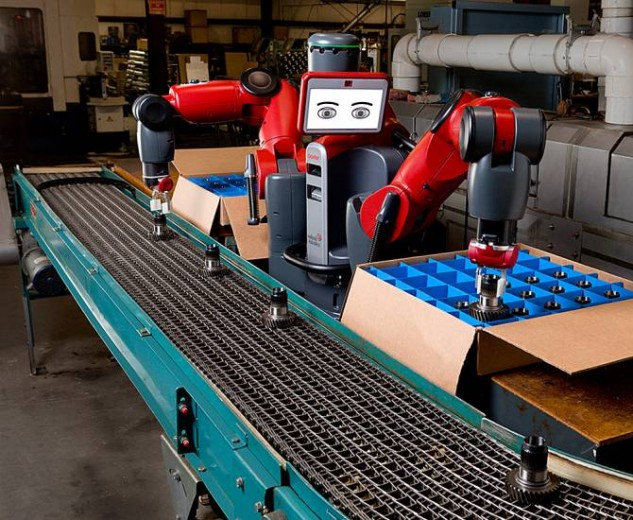
\includegraphics[width=0.6\textwidth]{../traspas/img/robot_industrial.jpg}
\label{fig:baxter}
\caption{Baxter en una cadena de embalaje}
\end{figure}

Fuera de las f�bricas se empezaron a usar en terrenos hostiles para el hombre, como las zonas radioactivas o en la exploraci�n espacial. 
Adem�s, actualmente se empieza a usar en otros entornos como la agricultura, el ocio y el entretenimiento. Por ejemplo, robots como Aibo de Sony (figura \ref{fig:aibo}) 
y en los hogares Roomba (figura \ref{fig:roomba}) para la limpieza de la casa, en los coches, con las funciones como aparcar o incluso de conducir solos (figura \ref{fig:google}).
Tambi�n se usan en los almacenes grandes como los de Amazon para transportar los productos de un lado a otro (figura \ref{fig:amazon})
\begin{figure}[htb]
\centering
\subfigure[]{\label{fig:roomba}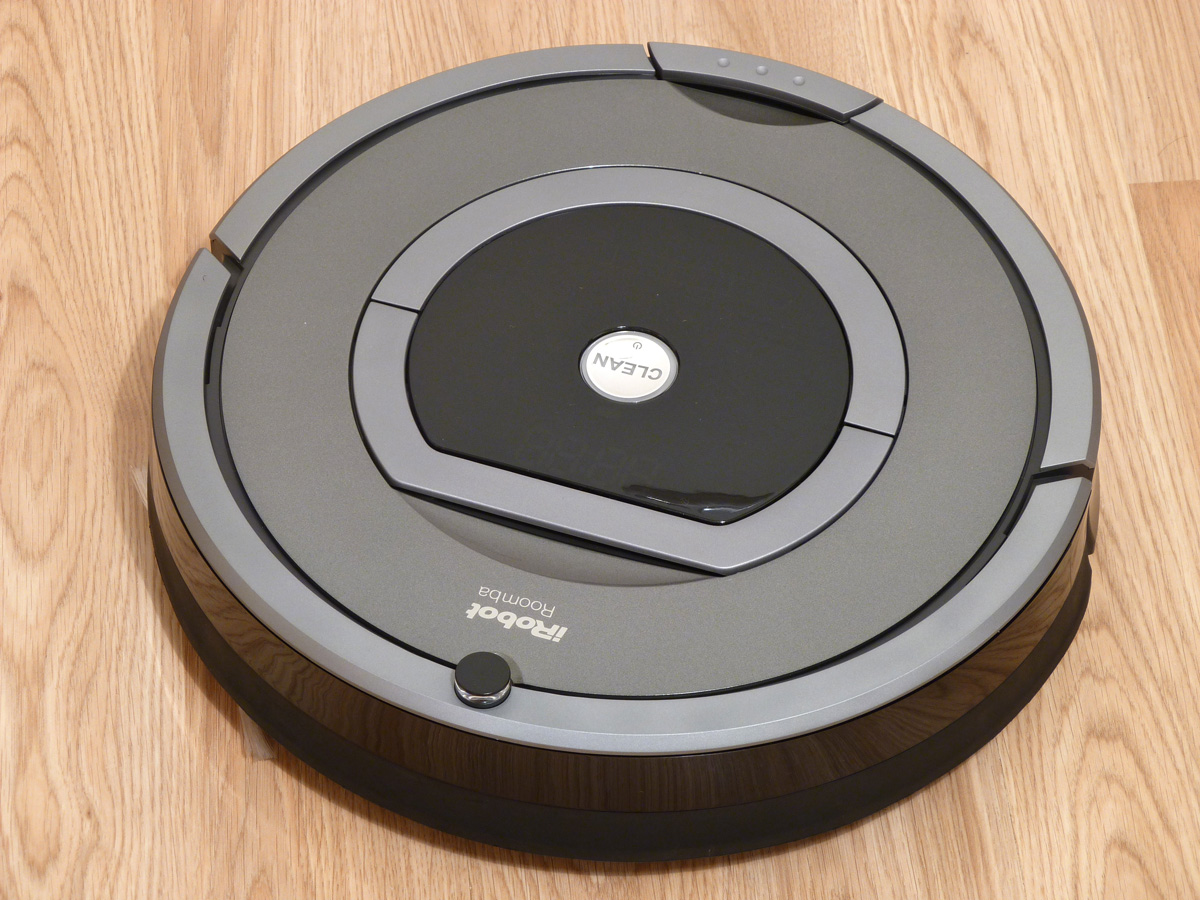
\includegraphics[width=0.4\textwidth]{./img/IRobot_Roomba_780.jpg}}
\hspace{1cm}
\subfigure[]{\label{fig:aibo}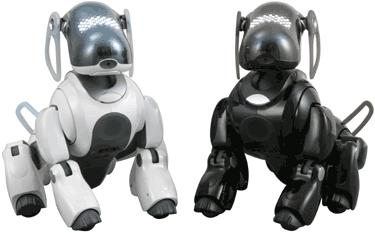
\includegraphics[width=0.4\textwidth]{./img/aibo.jpeg}}
\caption{Roomba de iRobot (a) y Aibo de Sony (b)}
\label{fig:roboejemplo1}
\end{figure}

\begin{figure}[htb]
\centering
\subfigure[]{\label{fig:google}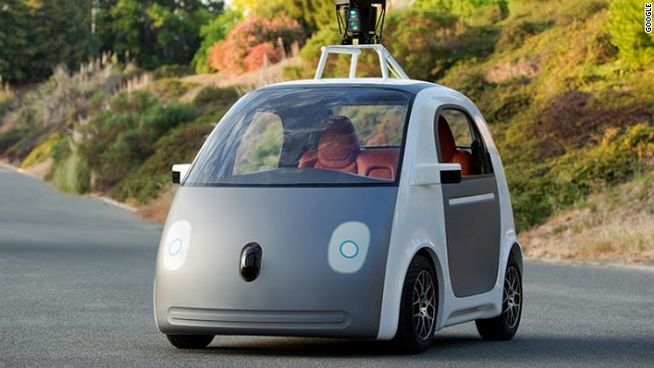
\includegraphics[width=0.48\textwidth]{../traspas/img/coche_google.jpg}}
\hspace{0.2cm}
\subfigure[]{\label{fig:amazon}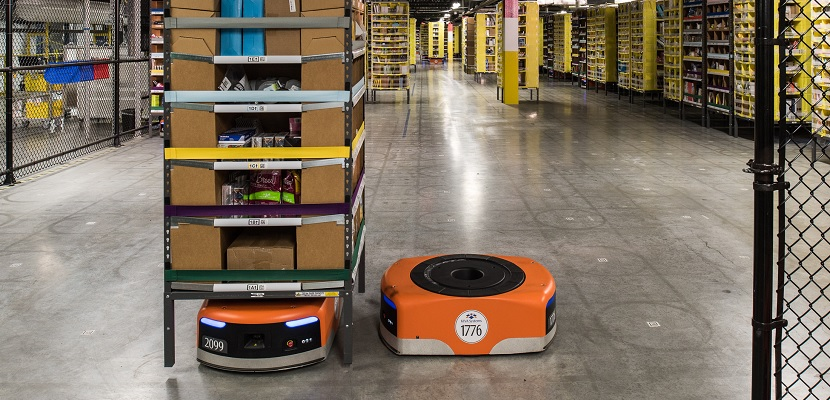
\includegraphics[width=0.48\textwidth]{./img/Robots-Amazon-2.jpg}}
\caption{GoogleCar (a) y Robots de Amazon (b)}
\label{fig:roboejemplo2}
\end{figure}

Actualmente hay robots que entienden emociones e interact�an con personas para hacerlas sentir mejor, como es el caso de 
Pepper\footnote{fuente: \url{https://www.aldebaran.com/en/Launch_Sales_of_Pepper}} (figura \ref{fig:pepper}) o incluso son capaces de realizar labores de recepcionista en un hotel en 
Jap�n\footnote{fuente: \url{http://cnnespanol.cnn.com/2015/07/18/inauguran-en-japon-el-primer-hotel-atendido-por-robots/}} (figura \ref{fig:hotel}).

\begin{figure}[htb]
\centering
\subfigure[]{\label{fig:pepper}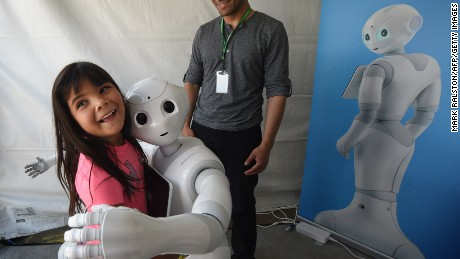
\includegraphics[width=0.48\textwidth]{./img/pepper.jpg}}
\hspace{0.2cm}
\subfigure[]{\label{fig:hotel}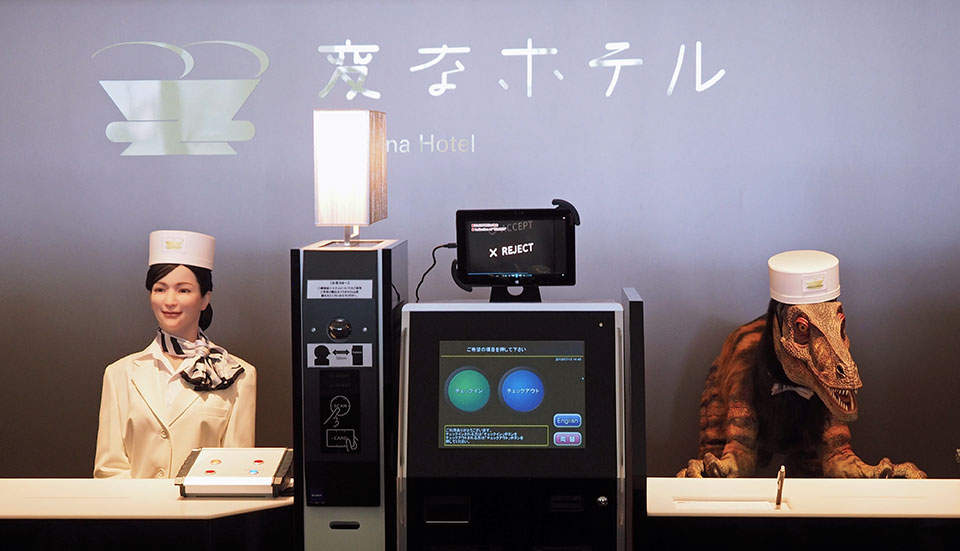
\includegraphics[width=0.48\textwidth]{./img/Hotel.jpg}}
\caption{Pepper (a) y Hotel rob�tico (b)}
\label{fig:roboejemplo3}
\end{figure}


Sin un \textit{software} todo esto ser�a impensable. \textit{Hardware} y \textit{software} deben trabajar juntos, 
no pueden existir el uno sin el otro. Un robot no puede funcionar sin un \textit{software} que le permita acceder a los datos de los sensores y actuadores, 
que le dote de inteligencia, le permita llevar a cabo algoritmos perceptivos y de toma de decisiones. En definitiva, sin un \textit{software}, un robot no difiere mucho de un pisapapeles muy caro.


El \textit{middleware} es un \textit{software} que asiste a una aplicaci�n para interactuar o comunicarse con otras aplicaciones, o paquetes de programas, redes, hardware y/o sistemas operativos. 
 �ste simplifica el trabajo de los programadores en la compleja tarea de generar las conexiones y sincronizaciones que son necesarias en los sistemas distribuidos. 
 Abstrae de la complejidad y heterogeneidad de las redes de comunicaciones subyacentes, as� como de los sistemas operativos, proporcionando una API para la f�cil 
 programaci�n y manejo de aplicaciones distribuidas.


 En los �ltimos a�os se han asentado varios \textit{middlewares} en el campo de la rob�tica, que simplifican la creaci�n de aplicaciones en ese �mbito.
\subsection{ROS}
ROS\footnote{Web: \url{http://www.ros.org/}} es un \textit{middelware} para el desarrollo de \textit{software} para robots, bajo
licencia de c�digo abierto y mantenido por OSRF\footnote{\url{http://www.osrfoundation.org/}} (\textit{Open Source Robotics Foundation}). Provee servicios t�picos de un sistema operativo, como son
abstracci�n de acceso al hardware, control de bajo nivel para dispositivos, mecanismos
de paso de mensajes entre procesos y nodos (\textit{Topics Services Actions}) y mantenimiento de paquetes. Se propone como una capa mediadora entre
el robot y sistema operativo por un lado y el programador por otro. Es un \textit{software} multi-plataforma aunque actualmente s�lo la versi�n para
Linux es considerada estable. Por el momento, los lenguajes
de desarrollo soportados son C++, Python y LISP, aunque hay intenci�n de soportar algunos
m�s proporcionando librer�as cliente que puedan acceder al API de ROS, como es el caso de \texttt{roslibjs} que da soporte para JavaScript

Su dise�o va en la l�nea de ser lo m�s ligero posible y capaz
de ser integrado o utilizado f�cilmente por otros sistemas existentes, para fomentar la
reutilizaci�n de \textit{software} rob�tico. Sus librer�as se han dise�ado para ofrecer
interfaces claros y limpios. 

Otro punto a destacar es su sistema de gesti�n del \textit{software}, que provee mecanismos
para la distribuci�n e integraci�n de paquetes de \textit{software} con funcionalidad determinada. 
Incluye la estructura de directorios que un paquete debe tener y c�mo deben
usarse, descripciones de la funcionalidad contenida, y detalles de alto nivel de c�mo se
comunica dicho \textit{software} con otras piezas.

Se ha extendido tanto, como demuestran sus aproximadamente 9 millones de paquetes descargados de unas 70.000 IPs diferentes s�lo en Mayo de 2015, que se ha convertido en un est�ndar de facto.

\subsection{JdeRobot}
JdeRobot \cite {jderobot} es un \textit{middelware} para el desarrollo de aplicaciones orientadas a la rob�tica,
dom�tica y visi�n artificial (ejemplos en la figura \ref{fig:jderobot}). La versi�n actual de JdeRobot es la 5.3. Esta plataforma
est� dise�ada para facilitar la programaci�n de \textit{software} que dote de cierta inteligencia
a hardwares tan distintos como c�maras, actuadores y en general robots de todo tipo.
Los componentes est�n escritos en C++, Python, Java... y basadas en un entorno de
componentes distribuidos. Cada aplicaci�n est� construida con la concurrencia de varios
componentes as�ncronos. Cada componente puede ejecutarse en una m�quina distinta
y para su interconexi�n se usa el \textit{middelware} de comunicaciones ICE \cite {ice}.

JdeRobot simplifica el acceso a los dispositivos hardware desde el programa principal.
As�, obtener una medida de un sensor u ordenar un movimiento a un motor es tan simple
como llamar a una funci�n local.

\begin{figure}[htb]
\centering
\subfigure[]{\label{fig:uav_viewer}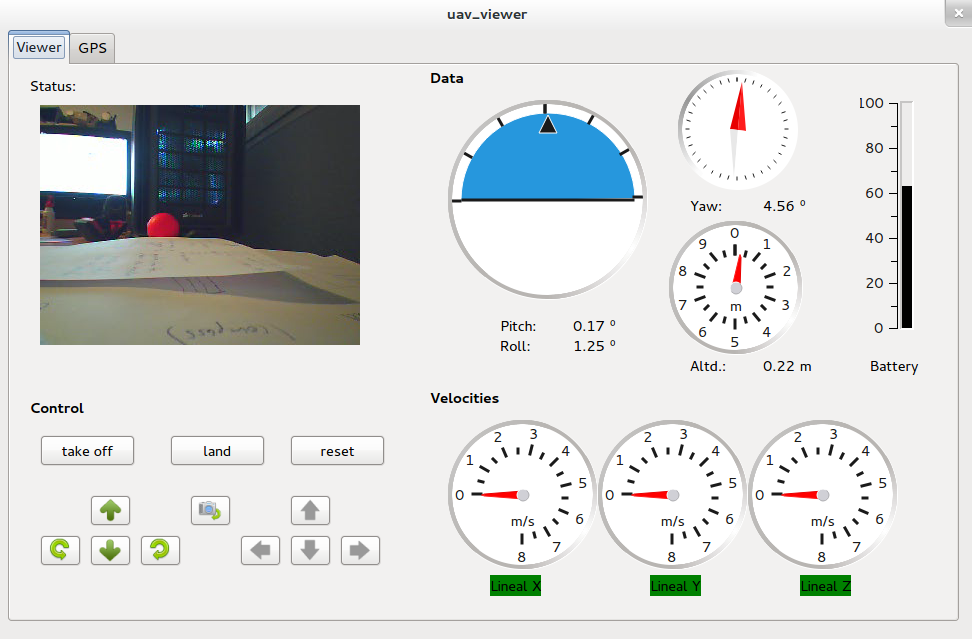
\includegraphics[width=0.4\textwidth]{./img/jde_uav_viewer.png}}
\hspace{1cm}
\subfigure[]{\label{fig:intro}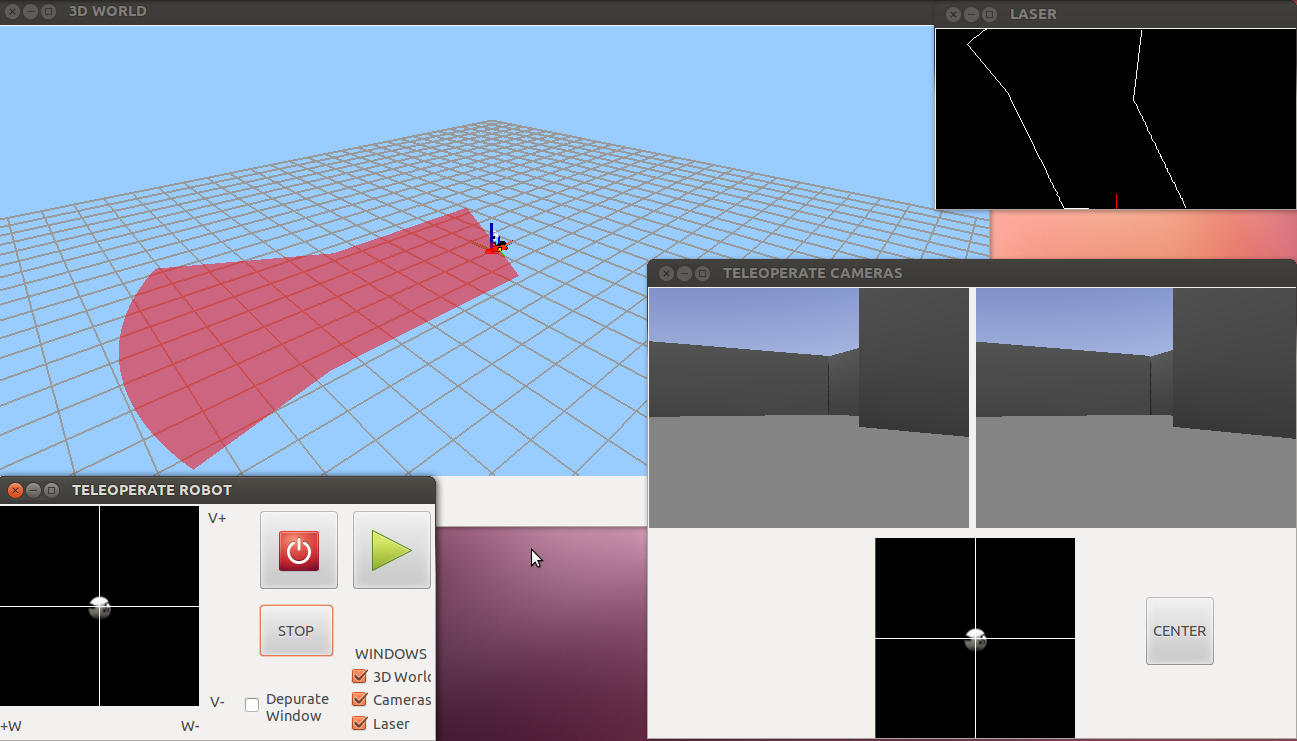
\includegraphics[width=0.4\textwidth]{./img/jde_introrob.png}}
\caption{Uav Viewer (a) e Introrob (b)}
\label{fig:jderobot}
\end{figure}

Los componentes desarrollados por JdeRobot pueden conectarse a sensores y actuadores
reales o simulados. Estas conexiones pueden ser locales (dentro de la misma m�quina), 
a nivel de red local o usando Internet.

Actualmente se usa tanto en docencia como en investigaci�n en la URJC y ha formado parte del \textit{Google Summer of Code 2015}\footnote{\url{https://www.google-melange.com/gsoc/org2/google/gsoc2015/jderobot}}
, programa donde Google remunera a los estudiantes  mayores de 18 a�os que completan un proyecto de programaci�n de \textit{software} libre durante ese periodo de verano.

\subsubsection{ICE}

ZeroC ICE \cite{ice}\cite{ice_manual} (\textit{Internet Communications Engine}) es un \textit{middleware} de comunicaciones, \textit{software} libre, orientado al desarrollo de aplicaciones 
distribuidas que permite a los programadores centrarse en la l�gica de la aplicaci�n,
haciendo transparentes detalles como abrir conexiones, retransmitir paquetes por la red, serializaci�n, etc.
Es compatible con lenguajes como C++, Java, Python, PHP o C\#, haciendo posible que dos m�quinas
con procesos escritos en lenguajes distintos puedan comunicarse.

ICE ofrece mecanismos de RPC (llamadas a procedimientos remotos), tanto as�ncronas como s�ncronas, control de hilos sin necesidad
de preocuparnos por regiones cr�ticas en cuanto a accesos a memoria, posibilidad de elegir entre TCP,
UDP o SSL como protocolos de nivel de transporte, y un lenguaje propio llamado \textit{slice} para establecer
interfaces de comunicaci�n. Con \textit{slice} se pueden definir clases, m�todos, tipos definidos por el usuario como
diccionarios, secuencias o enumeraciones, herencias, excepciones, etc. Tras definir una interfaz, es necesario
traducirlo al lenguaje concreto de nuestra aplicaci�n mediante unos compiladores llamados ice2``lenguaje''\cite{slicecomp} ya incluidos en la instalaci�n, por ejemplo, \texttt{ice2cpp, ice2python}. 

La versi�n utilizada en este proyecto es la 3.5.1.

\section{Tecnolog�as Web}
La principal manera de acceder a Internet es mediante el navegador para ver p�ginas web y para ello se utiliza el protocolo HTTP. Las aplicaciones web tienen un lado cliente y un lado servidor. Los lenguajes m�s usados en el lado del cliente 
son HTML, para explresar el contenido de las p�ginas, JavaScript para interactuar con ellas y CSS para modificar su apariencia. En este punto vamos a tratar cada una de estas tecnolog�as. Una de las principales
ventajas es que son multiplataforma y de la mano de los \textit{smartphones} se han convertido en una verdadera revoluci�n digital. Actualmente \textit{World Wide Web Consortium} (W3C) est� elaborando una API
 para permitir a las aplicaciones del navegador realizar llamadas de voz, chat de v�deo y uso compartido de archivos P2P sin plugins, llamada WebRTC\footnote{\url{https://webrtc.org/}}.

Internet es un conjunto descentralizado de redes de comunicaci�n interconectadas que utilizan la familia de protocolos TCP/IP, 
lo cual garantiza que las redes f�sicas heterog�neas que la componen funcionen como una red l�gica �nica de alcance mundial. Naci� a partir de una red denominada ARPANET, dise�ada y desarrollada en 1969 para el Departamento de 
Defensa de Estados Unidos, creada para mantener la comunicaci�n entre computadoras en caso de guerra. 

Estados Unidos fue capaz de desarrollar una red que funcionara (la antecesora de la actual Internet) y 
los usuarios acad�micos e investigadores que ten�an acceso a ella empezaron a emplearla constantemente. 
Los desarrolladores de Internet en Estados Unidos, el Reino Unido y Escandinavia, en respuesta a las presiones del mercado, empezaron a poner el \textit{software} de IP 
(\textit{Internet Protocol}) en todo tipo de computadoras, llegando a ser un est�ndar. Al mismo tiempo que Internet se consolidaba, muchas 
compa��as y otras organizaciones empezaron a construir redes privadas usando los mismos protocolos de ARPAnet, por lo que los usuarios de una red podr�an comunicarse con 
usuarios de otra. 

Actualmente se usa para casi todo, desde buscar direcciones en un mapa (figura \ref{fig:maps}), enterarse de las noticias viendo el peri�dico (figura \ref{fig:elpais}), 
relacionarse con otras personas (figura \ref{fig:facebook}) o incluso han cambiado la forma en la que vemos la televisi�n (figura \ref{fig:netflix}).


\begin{figure}[htb]
\centering
\subfigure[]{\label{fig:maps}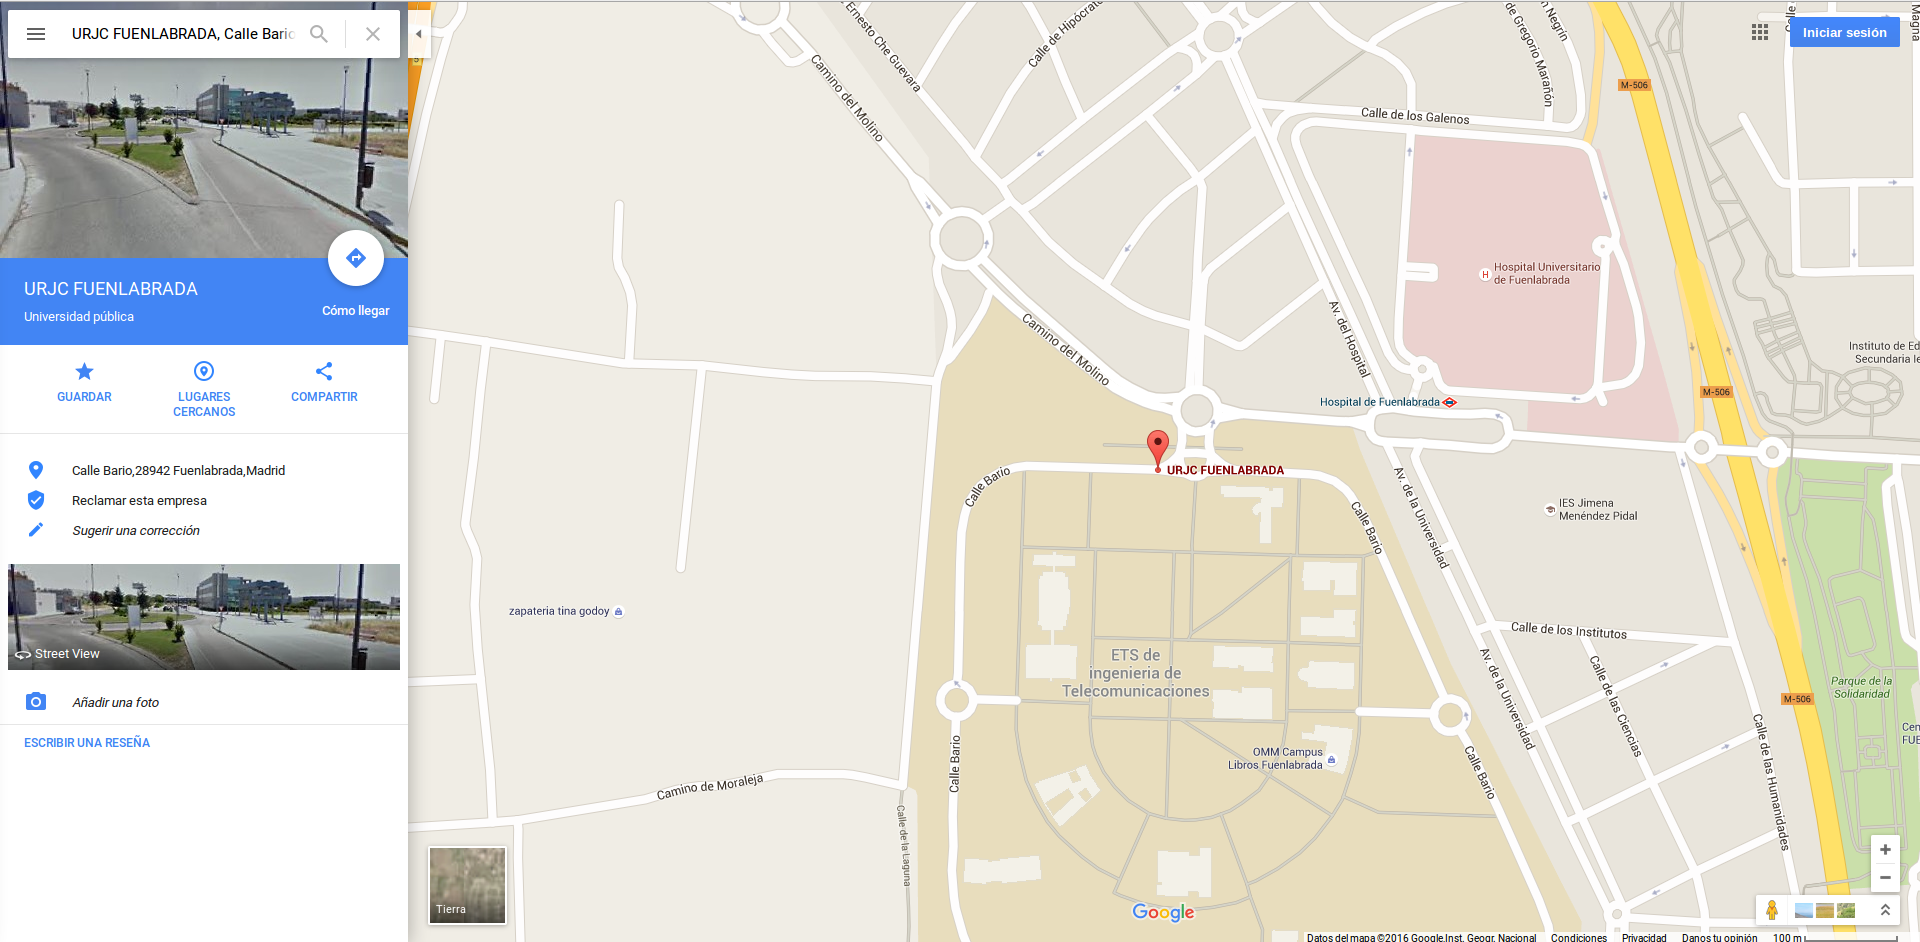
\includegraphics[width=0.4\textwidth]{../traspas/img/maps.png}}
\hspace{1cm}
\subfigure[]{\label{fig:facebook}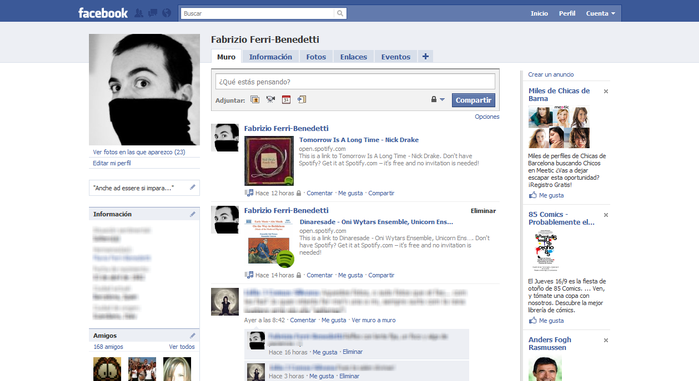
\includegraphics[width=0.4\textwidth]{../traspas/img/facebook-9.png}}
\caption{Google Maps (a) y Facebook (b)}
\label{fig:htmlejemplo1}
\end{figure}

\begin{figure}[htb]
\centering
\subfigure[]{\label{fig:elpais}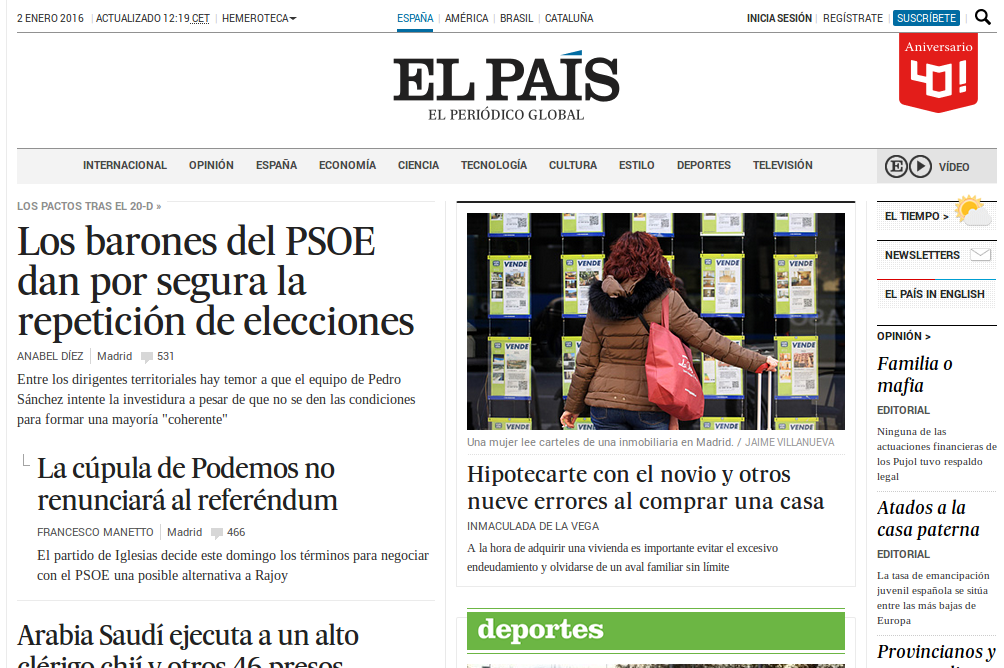
\includegraphics[width=0.4\textwidth]{../traspas/img/elpais.png}}
\hspace{1cm}
\subfigure[]{\label{fig:netflix}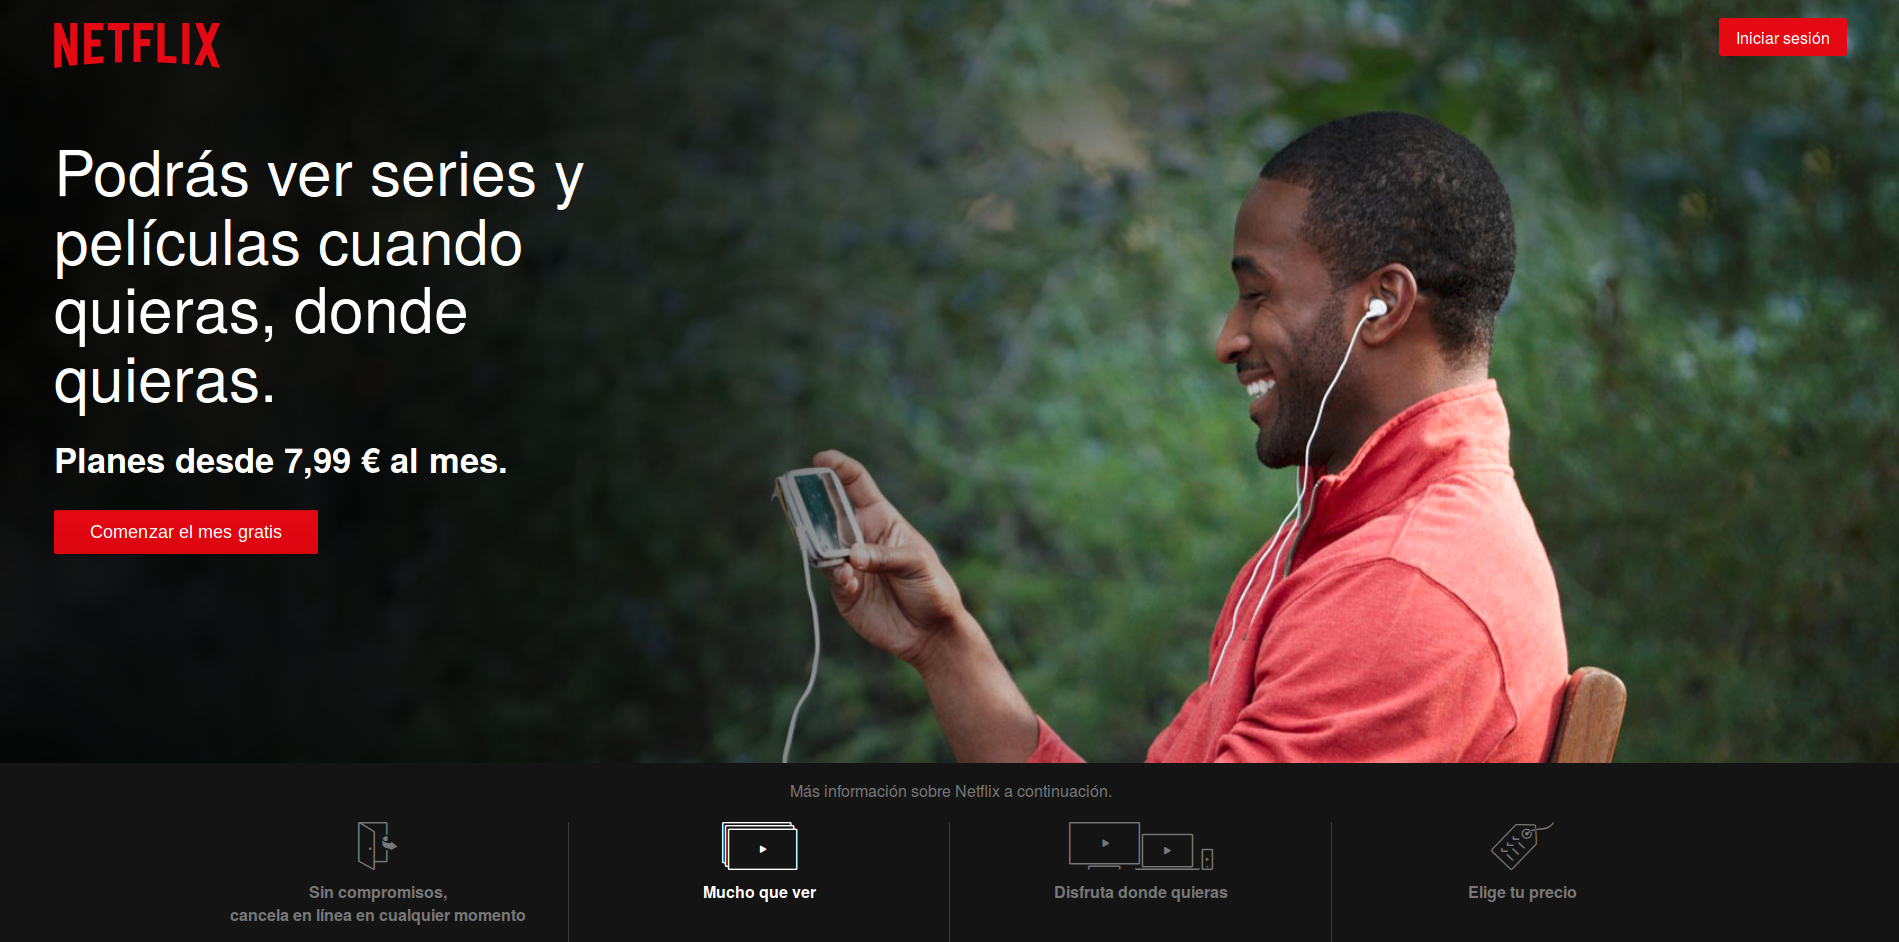
\includegraphics[width=0.4\textwidth]{../traspas/img/netflix.png}}
\caption{El Pa�s (a) y Netflix (b)}
\label{fig:htmloejemplo2}
\end{figure}

\subsection{HTTP}
Este protocolo fue desarrollado por el \textit{World Wide
Web Consortium}\footnote{Web: \url{http://www.w3.org/}} y la \textit{Internet Engineering Task Force}. En 1999 se public� la versi�n 1.1
usada en la actualidad. HTTP define la sintaxis y la sem�ntica que utilizan los elementos
de \textit{software} de la arquitectura web (clientes, servidores, proxies) para comunicarse. Es un protocolo orientado a transacciones y 
sigue el esquema petici�n-respuesta entre un cliente y un servidor (figura \ref{fig:httpclient-serv}). Al cliente que efect�a la petici�n (un navegador web) se lo 
conoce como \textit{user agent} (agente del usuario). A la informaci�n transmitida se le llama recurso y se identifica mediante un localizador uniforme de recursos (URL). 
El recurso es el resultado de la ejecuci�n de un programa, una consulta a una base de datos, la traducci�n autom�tica de un documento, etc.

\begin{figure}[htb]
\centering
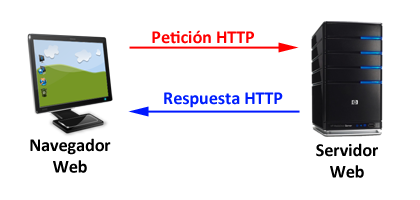
\includegraphics[width=0.8\textwidth]{./img/HTTPclient-serv.png}
\caption{Comunicaci�n cliente servidor en HTTP.} \label{fig:httpclient-serv}
\end{figure}

Es un protocolo sin estado, es decir, que no guarda ninguna informaci�n sobre
conexiones anteriores.

\subsection{HTML}
HTML significa Lenguaje de Marcado para Hipertextos (\textit{HyperText Markup Language}), y es el bloque de construcci�n m�s b�sico de una p�gina web. Se usa para crear 
y representar visualmente una p�gina web. Determina el contenido de la p�gina web, pero no su funcionalidad. Consta de etiquetas para delimitar los bloques (figura \ref{fig:html-example})

Es un est�ndar a cargo de la W3C\footnote{Web: \url{http://www.w3.org/}}, organizaci�n dedicada a la estandarizaci�n de casi todas las tecnolog�as ligadas a la web. 
Se considera el lenguaje web m�s importante siendo su invenci�n crucial en la aparici�n, 
desarrollo y expansi�n de la \textit{World Wide Web}. Es el est�ndar que se ha impuesto en la visualizaci�n de p�ginas web y es el que todos los navegadores actuales han adoptado.

A lo largo de sus diferentes versiones, se han incorporado y suprimido diversas caracter�sticas, 
con el fin de hacerlo m�s eficiente y facilitar el desarrollo de p�ginas web compatibles con distintos navegadores y plataformas (PC de escritorio, 
port�tiles, tel�fonos inteligentes, tabletas, etc.). No obstante, para interpretar correctamente una nueva versi�n de HTML, los desarrolladores de navegadores 
web deben incorporar estos cambios.  As� mismo, las p�ginas escritas 
en una versi�n anterior de HTML deber�an ser actualizadas o reescritas, lo que no siempre se cumple. 
Es por ello que ciertos navegadores a�n mantienen la capacidad de interpretar p�ginas web de versiones HTML anteriores. Por estas razones, 
a�n existen diferencias entre distintos navegadores y versiones al interpretar una misma p�gina web.

\begin{figure}[htb]
\centering
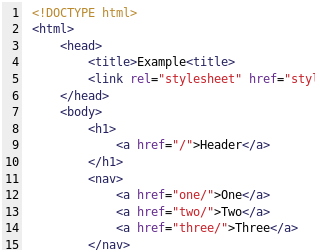
\includegraphics[width=0.5\textwidth]{./img/HTML_source_code_example.png}
\caption{Ejemplo de c�digo HTML.} \label{fig:html-example}
\end{figure}

El origen de HTML se remonta a 1980, cuando el f�sico Tim Berners-Lee, trabajador del CERN (Organizaci�n Europea para la Investigaci�n Nuclear) 
propuso un nuevo sistema de "hipertexto" para compartir documentos. Tras finalizar el desarrollo, Tim Berners-Lee lo present� a una convocatoria organizada 
para desarrollar un sistema de "hipertexto" para Internet. Despu�s de unir sus fuerzas con el ingeniero de sistemas Robert Cailliau, 
presentaron la propuesta ganadora llamada WorldWideWeb (W3). El primer documento formal con la descripci�n de HTML se public� en 1991 bajo el nombre HTML Tags (Etiquetas HTML).

La primera propuesta oficial para convertir HTML en un est�ndar se realiz� en 1993 por parte del organismo IETF (\textit{Internet Engineering Task Force}). Aunque no consiguieron convertirse en est�ndar oficial.

En 1995, el organismo IETF organiza un grupo de trabajo de HTML y consigue publicar, 
el 22 de septiembre de ese mismo a�o, el est�ndar HTML 2.0. A pesar de su nombre, HTML 2.0 es el primer est�ndar oficial de HTML.

A partir de 1996, los est�ndares de HTML los publica otro organismo de estandarizaci�n llamado W3C (\textit{World Wide Web Consortium}\footnote{Web: \url{http://www.w3.org/}}). 
La versi�n HTML 3.2 se public� el 14 de Enero de 1997. Esta revisi�n incorpora \textit{applets} de Java y texto que fluye alrededor de las im�genes.


HTML 4.0 se public� el 24 de abril de 1998
y supone un gran salto desde las versiones anteriores. Entre sus novedades m�s destacadas se encuentran las hojas de estilos CSS, 
la posibilidad de incluir peque�os programas o \textit{scripts} en las p�ginas web, mejora de la accesibilidad de las p�ginas dise�adas, tablas complejas y mejoras en los formularios.

Desde la publicaci�n de HTML 4.01, la actividad de estandarizaci�n de HTML se detuvo y el W3C se centr� en el desarrollo del est�ndar XHTML. 
Por este motivo, en el a�o 2004, las empresas Apple, Mozilla y Opera mostraron su preocupaci�n por la falta de inter�s del W3C en HTML y 
decidieron organizarse en una nueva asociaci�n llamada WHATWG (\textit{Web Hypertext Application Technology Working Group}).

Debido a la fuerza de las empresas que forman el grupo WHATWG y a la publicaci�n de los borradores de HTML 5.0, 
en marzo de 2007 el W3C\footnote{Web: \url{http://www.w3.org/}} 
decidi� retomar la actividad estandarizadora de HTML. La versi�n definitiva de la quinta revisi�n del est�ndar se public� en octubre de 2014\footnote{\url{http://www.w3.org/TR/2014/REC-html5-20141028/.}} 
Esta revisi�n incluye nuevas caracter�sticas como pueden ser la geolocalizaci�n (hasta la llegada de los \textit{smartphones} no era necesaria) y soporte para v�deos y audios sin necesidad de plugins externos. 



\subsection{JavaScript}
JavaScript (abreviado com�nmente ``JS'') es un lenguaje de programaci�n interpretado, 
dialecto del est�ndar ECMAScript. Se define como orientado a objetos, basado en prototipos, imperativo, d�bilmente tipado y din�mico. Se utiliza principalmente en su forma del lado del cliente (\textit{client-side}), que es lo que usamos en este TFG 
y que describiremos en detalle en el cap�tulo 3, 
se ejecuta dentro del navegador web, que contiene el int�rprete de JavaScript, permitiendo mejoras en la interfaz de usuario y p�ginas web din�micas.

La idea de JavaScript surgi� cuando a principios de los 90 con unas aplicaciones web cada vez m�s complejas y una velocidad de navegaci�n tan lenta, 
surgi� la necesidad de un lenguaje de programaci�n que se ejecutara en el navegador del usuario y Brendan Eich, 
un programador que trabajaba en Netscape, cre� LiveScript.

Posteriormente, Netscape firm� una alianza con Sun Microsystems para el desarrollo del nuevo lenguaje de programaci�n. 
Adem�s, justo antes del lanzamiento Netscape decidi� cambiar el nombre por el de JavaScript. La raz�n del cambio de 
nombre fue exclusivamente por marketing, ya que Java era la palabra de moda en el mundo inform�tico y de Internet de la �poca.

La primera versi�n de JavaScript fue un completo �xito. Al mismo tiempo, Microsoft lanz� JScript con su navegador Internet Explorer 3, el cual era una copia de JavaScript 
al que le cambiaron el nombre para evitar problemas legales. Para evitar una guerra de tecnolog�as, Netscape decidi� que lo mejor ser�a estandarizar el lenguaje JavaScript. 
De esta forma, en 1997 se envi� la especificaci�n JavaScript 1.1 al organismo ECMA\footnote{\url{http://www.ecma-international.org/}} (\textit{European Computer Manufacturers Association}).

ECMA cre� el comit� TC39 con el objetivo de ``estandarizar de un lenguaje de \textit{script} multiplataforma e 
independiente de cualquier empresa''. El primer est�ndar que cre� el comit� TC39 se denomin� ECMA-262, en el que se defini� por primera vez el lenguaje ECMAScript.

Al principio muchos desarrolladores renegaban del lenguaje porque el p�blico al que va dirigido lo formaban 
publicadores de art�culos y dem�s aficionados, entre otras razones. La llegada de AJAX (permite interacciones ligeras entre navegador y servidor web) devolvi� JavaScript a la fama y 
atrajo la atenci�n de muchos otros programadores. Como resultado de esto hubo una proliferaci�n de un conjunto de entornos y 
librer�as de �mbito general, mejorando las pr�cticas de programaci�n con JavaScript, y aumentado el uso de JavaScript fuera de los navegadores web, 
como se ha visto con la proliferaci�n de entornos JavaScript del lado del servidor. En enero de 2009, el proyecto CommonJS fue 
inaugurado con el objetivo de especificar una librer�a para uso de tareas comunes principalmente para el desarrollo fuera del navegador web. En mayo de 2009 surge Node.js \footnote{\url{https://nodejs.org/en/}} que permite ejecutar 
aplicaciones JavaScript en el lado del servidor.

En Junio de 2015 se cerr� y public� el est�ndar ECMAScript\footnote{\url{http://www.ecma-international.org/publications/standards/Ecma-262.htm}} 619 20 (�ltima versi�n hasta la fecha) con un soporte irregular entre navegadores y 
que dota a JavaScript de caracter�sticas avanzadas que se echaban de menos y que son de uso habitual en otros lenguajes como, 
por ejemplo, m�dulos para organizaci�n del c�digo, verdaderas clases para POO, expresiones de flecha, iteradores, generadores o promesas para programaci�n as�ncrona.

M�s all� del lenguaje hay bloques de funcionalidad ya resuelta, bibliotecas en JavaScript que se ver�n con mas detalle en el cap�tulo 3.

JQuery\cite{jquery} es una biblioteca de JavaScript, creada inicialmente por John Resig, que permite simplificar el uso de JavaScript. La primera versi�n de jQuery se present� en Febrero de 2006. Esta librer�a sorprendi� gratamente a la comunidad de desarrolladores web puesto 
que simplificaba en gran medida la programaci�n de c�digo JavaScript para interactuar, tanto con los elementos del DOM como para gestionar los diferentes 
eventos que se producen en la visita de una p�gina web. Desde su publicaci�n, la librer�a ha evolucionado solucionando errores, optimizando su c�digo y 
ampliando las funcionalidades ofrecidas. Actualmente est� la versi�n 2.14 y cuenta con el apoyo de Google, Microsoft, IBM,...


WebGL\cite{webgl} es una especificaci�n est�ndar que est� siendo desarrollada actualmente para mostrar gr�ficos en 3D en navegadores web. T�cnicamente es un API para JavaScript que permite usar la implementaci�n nativa de OpenGL ES 2.0 que ser� incorporada en los navegadores. 
WebGL es gestionado por el consorcio de tecnolog�a sin �nimo de lucro Khronos Group\footnote{\url{https://www.khronos.org/}}. WebGL creci� desde los experimentos del canvas 3D comenzados Mozilla. El primero mostr� un prototipo de Canvas 3D en 2006. 
A finales de 2007, tanto Mozilla como Opera hab�an hecho sus propias implementaciones separadas. Notables primeras aplicaciones de WebGL son Google Maps y Zygote Body.

\section{Tecnolog�as web en middlewares rob�ticos}
Este TFG se sit�a a caballo entre los dos campos mencionados, rob�tica y tecnolog�as web. Algunos trabajos previos existentes en esta intersecci�n son los siguientes. 
\subsection{The Robot Management System}
El RMS\footnote{\url{http://wiki.ros.org/rms/}} (Robot Management System) es una herramienta que permite controlar desde una p�gina web robots que tengan el \textit{middleware} ROS. RMS en s� se refiere a un sistema de gesti�n web escrito en PHP que est� respaldado por una base de datos MySQL. 
El sistema utiliza un framework modelo-vista-controlador (MVC) a trav�s del popular framework CakePHP\footnote{\url{http://cakephp.org/}}. RMS est� escrito en forma independiente de 
la plataforma robot (el robot en s�) por lo que permite el control de una gran variedad de robots. Adem�s de ser multiplataforma, RMS permite usuario b�sico y gesti�n de accesos, 
gesti�n de la interfaz, gesti�n de contenidos, y los estudios de los usuarios remotos. RMS se desarrolla como parte del esfuerzo por desarrollar herramienta de la ``Robot Web Tools''\footnote{\url{http://robotwebtools.org/}}.
En la Figura \ref{fig:rms} hay un ejemplo de c�mo se ve dicha aplicaci�n.

\begin{figure}[htb]
\centering
\subfigure[]{\label{fig:rms1}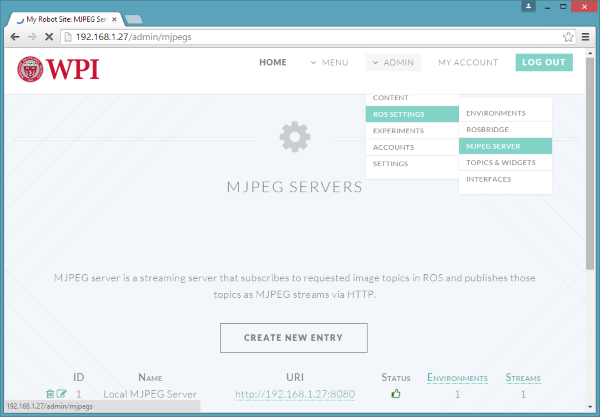
\includegraphics[width=0.4\textwidth]{./img/rms1.png}}
\hspace{1cm}
\subfigure[]{\label{fig:rms2}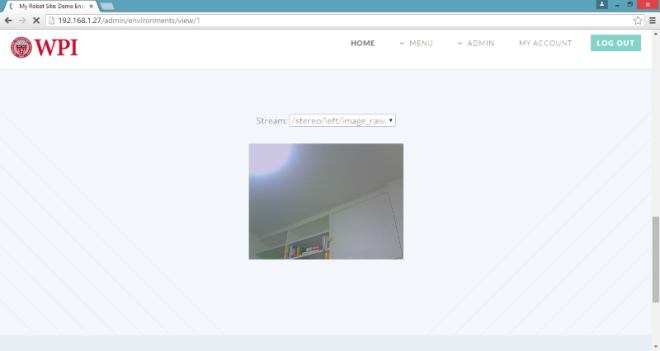
\includegraphics[width=0.4\textwidth]{./img/rms2.png}}
\caption{Men� de RMS (a) y C�mara a trav�s de RMS (b)}
\label{fig:rms}
\end{figure}
\subsection{Surveillance 4.0 (URJC)}
\label{ssec:s4}

\textbf{Surveillance 4.0} \cite{TFGsurveillance4.0} \cite{surveillance4.0} fue desarrollado por Daniel Castellano como su Proyecto
Fin de Carrera. Esta aplicaci�n contaba con varios sensores de distinto tipo (humedad,
temperatura, gas, etc) que se conectaban inal�mbricamente con un nodo central situado
en una Raspberry Pi. La conexi�n inal�mbrica se hac�a mediante transmisores Zigbee\footnote{\url{http://www.zigbee.org/}}
con un protocolo propio llamado WHAP. El nodo central recib�a los datos de los sensores y
los mostraba mediante un servidor web que corr�a en la misma m�quina. La aplicaci�n web
se desarroll� en Python usando el entorno de desarrollo web Django. En Surveillance 4.0, los
valores de los sensores se guardaban en una base de datos que la aplicaci�n web consultaba
cuando era necesario. Adem�s, esta versi�n inclu�a un \textit{streaming} de v�deo utilizando
el \textit{software} de c�digo abierto M-JPEG Streamer. En la figura \ref{fig:surveillance4} se puede ver la aplicaci�n.

\begin{figure}[htb]
\centering
\subfigure[]{\label{fig:su41}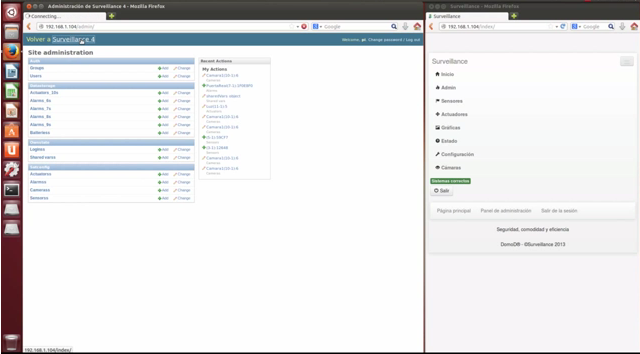
\includegraphics[width=0.7\textwidth]{./img/surveillance4.png}}
\hspace{1cm}
\subfigure[]{\label{fig:su42}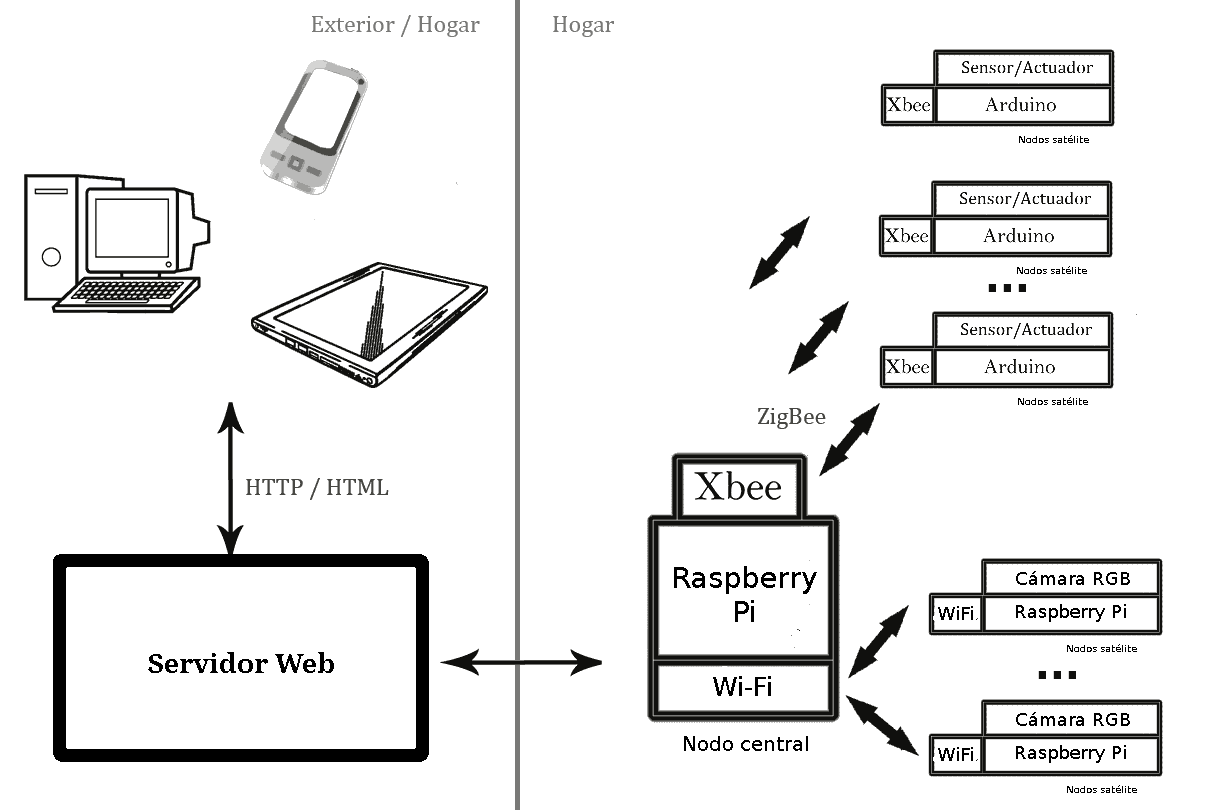
\includegraphics[width=0.7\textwidth]{../traspas/img/Esquema_s4.png}}
\caption{interfaz (a) y arquitectura (b)}
\label{fig:surveillance4}
\end{figure}



\subsection{Surveillance 5.1 (URJC)}
\label{ssec:s5}
\textbf{Surveillance 5.1} \cite{TFGsurveillance5.1} \cite{surveillance5.1} fue desarrollado por Edgar Barrero como su Trabajo Fin de Grado. 
Esta aplicaci�n obten�a un flujo de im�genes de una c�mara web, un flujo de im�genes de profundidad de un sensor Kinect, 
adem�s de datos de un sensor de humedad y de interaccionar con un actuador. La aplicaci�n web
se desarroll� en Ruby sobre Rails. En Surveillance 5.1, el servidor web se conectaba a los componente de JdeRobot mediante sus interfaces ICE.
La aplicaci�n web refrescaba estos datos mediante peticiones AJAX.  En la figura \ref{fig:surveillance5} se puede ver la aplicaci�n.

\begin{figure}[htb]
\centering
\subfigure[]{\label{fig:su51}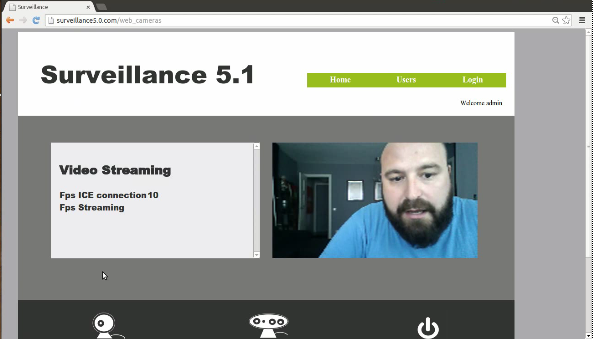
\includegraphics[width=0.7\textwidth]{./img/surveillance5.png}}
\hspace{1cm}
\subfigure[]{\label{fig:su52}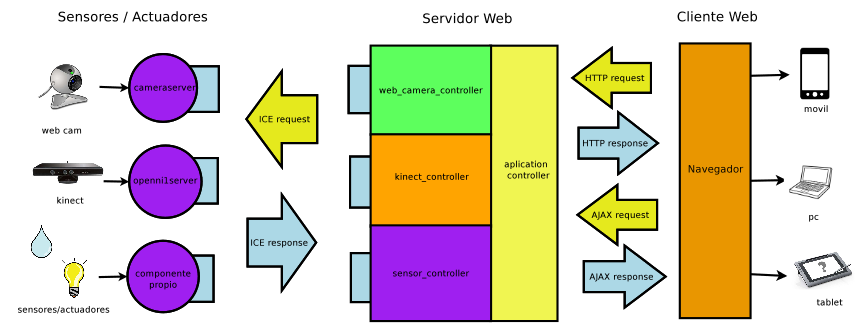
\includegraphics[width=0.7\textwidth]{../traspas/img/esquema_s5.png}}
\caption{interfaz (a) y arquitectura (b)}
\label{fig:surveillance5}
\end{figure}

\vspace{2cm}
En el Trabajo de Fin de Grado presentado en esta memoria se desarrollan seis clientes web: CameraViewJS, RGBDViewerJS, KobukiViewerJS, UavViewerJS, IntrorobKobukiJS e IntrorobUavJS, 
que son las versiones web de las herramientas de JdeRobot hom�nimas y que hablan directamente con los servidores que tiene JdeRobot para acceder a los sensores y robots a diferencia 
de los dos �ltimos antecedentes, que usan un servidor web como intermediario.


En el siguiente cap�tulo se presentan los objetivos de este TFG. En el cap�tulo de
Plataforma de Desarrollo se hace un resumen de las tecnolog�as usadas en los clientes.
En el cap�tulo de Dise�o e implementaci�n se profundiza en el dise�o y programaci�n de los clientes.
Las pruebas se detallan en el cap�tulo de Experimentos.
Por �ltimo, el cap�tulo de Conclusiones se hace un resumen de los objetivos logrados y se presentan futuras l�neas de trabajo.




\chapter{Objetivos y Metodolog�a}
\label{ch:Objetivos}

Una vez presentado el contexto general sobre el que se asienta este
trabajo, vamos a describir los
objetivos concretos que pretendemos resolver con la realizaci�n de
este TFG y los requisitos que han condicionado la soluci�n
desarrollada.


\section{Descripci�n del problema} \label{sec:descripcion}

El objetivo general del TFG consiste en crear versiones web de seis herramientas 
de JdeRobot muy utilizadas y que actualmente est�n programadas en C++ o 
Python con su propio interfaz gr�fico, que usa bibliotecas como QT o GTK y que s�lo se puede ejecutar en Linux. 
�stas versiones web van a ser multiplataforma (Linux, Android, IOS, Windows,...), van a usar el navegador web como interfaz gr�fico y nos va a 
permitir acceder a los sensores y actuadores sin un servidor web intermedio.

Este objetivo final lo hemos divido en cinco sub-objetivos:

\begin{enumerate}

\item \emph{CameraViewJS:} Creaci�n del cliente web similar a la herramienta \texttt{CameraView} para visualizar im�genes procedentes del servidor \texttt{Cameraserver}. 

\item \emph{RGBDViewerJS:} Creaci�n del cliente web similar a la herramienta RGBDViewer para visualizar datos de color y profundidad procedentes del servidor \texttt{Openni1Server}.
  
\item \emph{KobukiViewerJS:} Creaci�n de un teleoperador para poder ver, manejar y ver los datos de los sensores de los robots Kobuki y Pioneer del laboratorio de rob�tica de la URJC. Versi�n web de \texttt{KobukiViewer}
  
  
\item \emph{UavViewerJS:} Creaci�n del cliente web similar a la herramienta UavViewer para teleoperar drones tanto reales como simulados y ver los datos de sus sensores.
  
  
\item Creaci�n de dos herramientas que adem�s de mostrar los datos sensoriales del robot y ofrecer su teleoperaci�n, permite
 insertar c�digo que gobierna el comportamiento aut�nomo de robots Kobuki y drones (IntrorobKobukiJS e IntrorobUavJS). 

\end{enumerate}


Adem�s, se ha creado una p�gina web para contener a todos los clientes.

\section{Requisitos} \label{sec:requisitos}

Se deben satisfacer los siguientes requisitos:
\begin{itemize}
 \item Se tiene que usar la �ltima versi�n de JdeRobot, la 5.3.1.
 \item La comunicaci�n con los servidores de sensores y actuadores debe ser en tiempo real.
 \item No habr� servidores web intermedios, a diferencia de los antecedentes descritos en las secciones \ref{ssec:s4} y \ref{ssec:s5}.
 \item Debe ser lo suficientemente maduro para poder integrarse en el repositorio oficial de JdeRobot y ser usado por terceros f�cilmente.
\end{itemize}



\section{Metodolog�a y plan de trabajo}

Para el desarrollo de este TFG se ha seguido el m�todo de desarrollo en espiral. Este
sistema se basa en iteraciones sucesivas en la que cada bucle o iteraci�n representa un
conjunto de actividades. Estas actividades incluyen tal y como muestra la figura \ref{fig:espiral}: an�lisis
de los requerimientos del sistema, dise�o del mismo, implementaci�n y pruebas.



\begin{figure}[htbp]
\centering
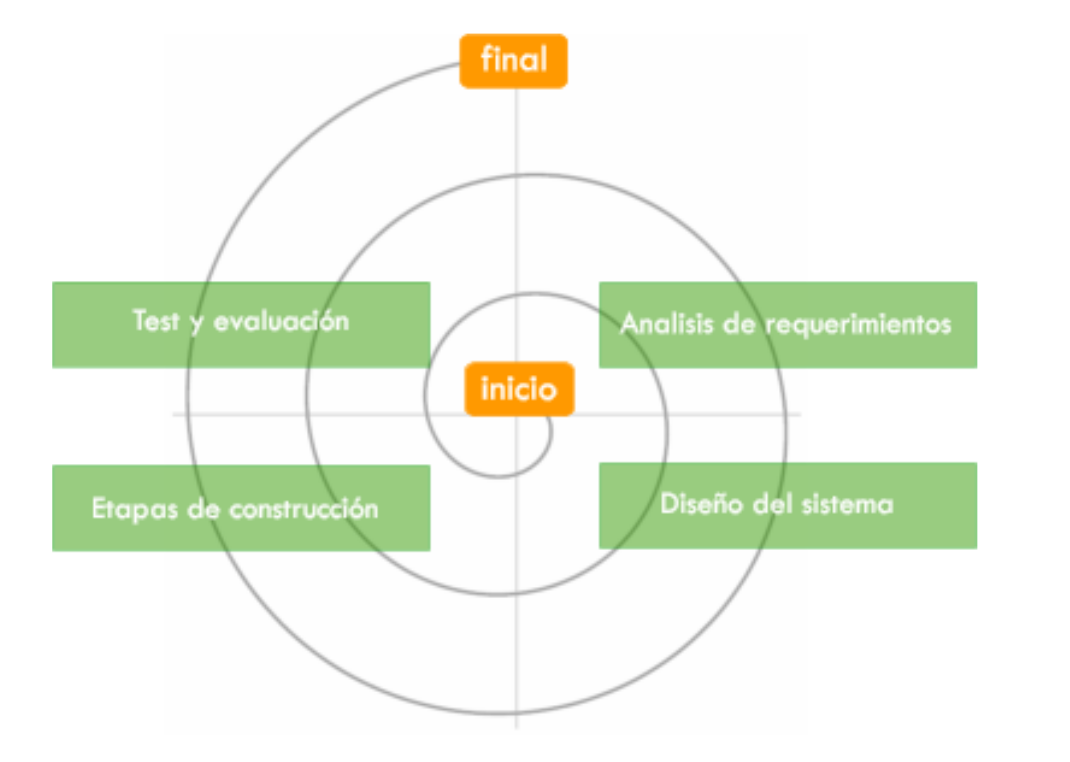
\includegraphics[width=0.8\textwidth]{img/espiral.png}
\caption{Modelo en espiral}
\label{fig:espiral}
\end{figure}

�ste TFG se ha ido documentando en un Mediawiki \cite{Mediawiki}. Este cuaderno de bit�cora
ha servido de apoyo a las reuniones con el tutor. Como complemento a
este Mediawiki se ha utilizado un repositorio p�blico svn \cite{Repositorio} donde se ha guardado y
est� accesible todo el c�digo fuente de este TFG.

El plan de trabajo, repartido en diferentes fases, con el fin de utilizar en cada fase nueva desarrollos ya creados en las anteriores, ha sido el siguiente: 

\begin{itemize}

\item \textbf{Aprendizaje de JdeRobot:} Primer contacto con la plataforma con el objetivo de saber c�mo funciona.

\item \textbf{Familiarizaci�n con las tecnolog�as web a utilizar:} Tiene el objetivo de aprender lo necesario sobre HTML, JavaScript, CSS, WebGL, ThreeJS. Primeros contactos con ICE-JS, 
\textit{middleware} utilizado para la comunicaci�n entre los clientes que se van a crear y los servidores de JdeRobot.

\item \textbf{Desarrollo de CameraViewJS:} En esta fase se crea el m�dulo que recibe el flujo de v�deo, que es la base del cliente.


\item \textbf{Desarrollo de RGBDViewerJS:} Se crea un m�dulo para recibir el flujo de im�genes de distancia, 
  juntando este flujo con otro de v�deo (ambos procedentes de un Kinect) mediante lo aprendido de ThreeJS se crea una representaci�n 
  en 3D de los datos recibidos por el sensor.
 
\item \textbf{KobukiViewerJS:} Se crea un m�dulo que permite interactuar con los motores de dicho robot 
  mediante un control con ThreeJS. Se incluyen dos flujos de v�deo que representan cada una de 
  las c�maras. Adem�s, se crean los m�dulos para recibir la informaci�n l�ser y odometr�a y una representaci�n 3D del robot movi�ndose seg�n los datos recibidos de la 
  odometr�a y se muestran los datos del l�ser.
  
\item \textbf{UavViewerJS:} Se crea un m�dulo que mediante dos controles iguales a los del teleoperador anterior permite mover el UAV. 
  Adem�s, se utiliza una representaci�n de indicadores de un avi�n para los datos de posici�n recibidos, al igual que se crea una representaci�n 3D.
  
  
\item \textbf{Introrob:} A \textit{KobukiViewerJS} y a \textit{UavViewerJS} se les a�ade la opci�n de poder agregar comportamiento aut�nomo en vez de teleoperarlos.


\item \textbf{Dise�o final de la web:} Se adapta el dise�o de la web para que sea vistoso y f�cil de manejar e integre todos los desarrollos anteriores.

\end{itemize}


Adem�s, se han hecho reuniones peri�dicas con el tutor para tener un seguimiento adecuado del desarrollo del mismo, que est�n documentadas en la bit�cora\footnote{\url{http://jderobot.org/Aitormf-tfg}}.



\chapter{Plataforma de Desarrollo}
\label{ch:PlataformaDesarrollo}

Una vez que hemos detallado los requisitos y objetivos de este
proyecto, vamos a describir en este cap�tulo la infraestructura empleada y en la que nos hemos apoyado.

\section{Simulador Gazebo}

Gazebo\cite {gazebo} es un simulador de software libre que incluye multitud de modelos
y motores de f�sica virtualizada y est� mantenido por OSRF\footnote{\url{http://www.osrfoundation.org/}} (\textit{Open Source Robotics Foundation}). 
Ofrece una interfaz gr�fica y control sobre los objetos
y el mundo (bastante realista) generado, adem�s de la creaci�n y modificaci�n de actuadores y sensores
personalizados. Permite probar algoritmos rob�ticos en mundos virtuales para madurarlos antes de llevarlos a robots reales, 
tambi�n permite impartir docencia en rob�tica sin tener los robots f�sicamente.
Por ejemplo, se pueden crear veh�culos con diferentes sensores o casas
con las que interactuar. En la figura \ref{fig:gazebo} se puede ver la interfaz gr�fica de Gazebo. Ha sido elegido por DARPA para su DRC\footnote{\url{http://www.theroboticschallenge.org/}}.

\begin{figure}[htb]
\centering
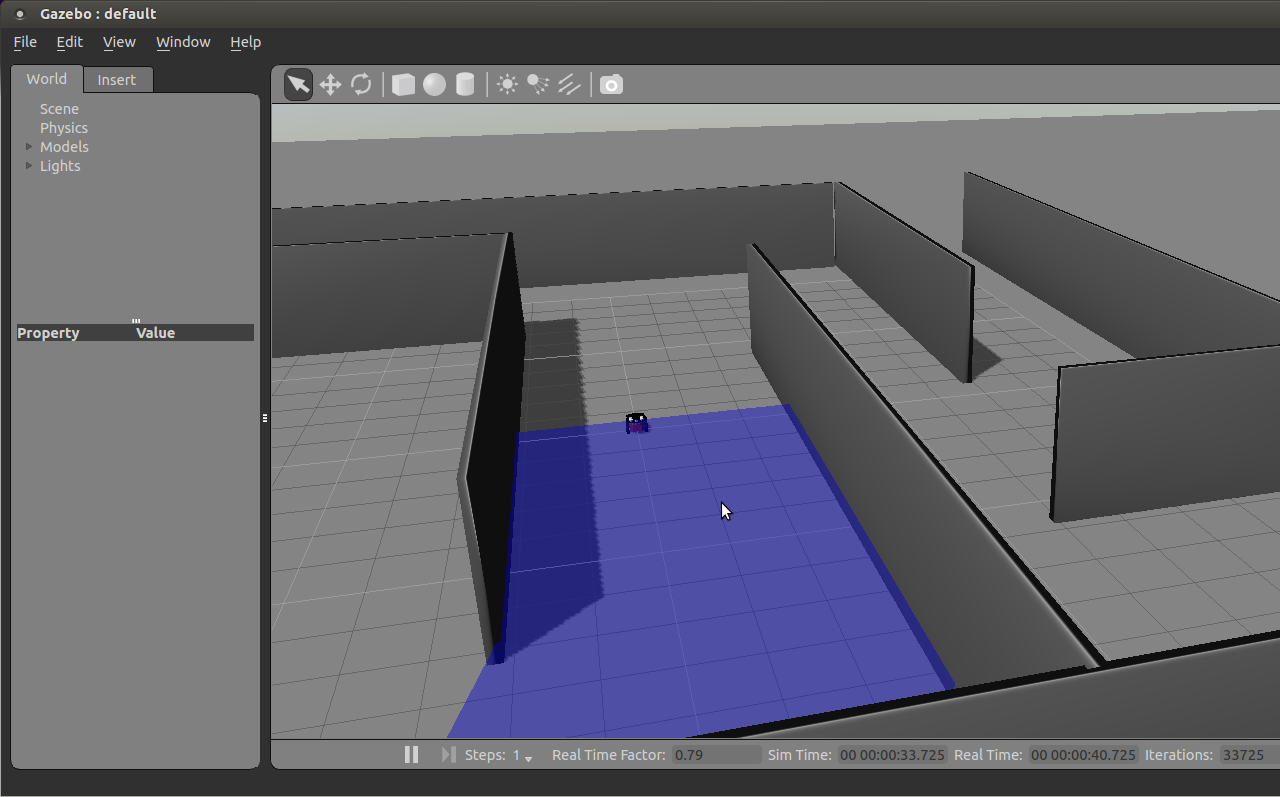
\includegraphics[width=0.8\textwidth]{./img/gazebo-sample.png}
\caption{Interfaz gr�fica del simulador Gazebo.} \label{fig:gazebo}
\end{figure}

Nosotros lo hemos utilizado tanto para probar los teleoperadores (UavViewerJS, KobukiViewerJS) como los introrob (IntrorobUavJS, IntrorobKobuki) 
con robots y drones simulados hasta que han sido lo suficientemente maduros.

\section{JdeRobot}
\label{sec:plat_jderobot}
A continuaci�n se detallan los componentes de \textit{JdeRobot}, plataforma ya introducida en el cap�tulo 1, utilizados en este TFG. 
Una de las ventajas que tiene es que el interfaz ICE del driver real y simulado es el mismo por lo que con cambiar la configuraci�n 
se puede usar uno u otro sin tener que volver a compilar las aplicaciones.

En este TFG se ha utilizado la versi�n 5.3.1.

\subsection{CameraServer + CameraView}

\texttt{Cameraserver}\cite {cameraserver} es un componente incluido en JdeRobot que ofrece \textit{streaming} de v�deo
de una o varias c�maras, tanto reales como simuladas. Usa GStreamer\cite {gstreamer} internamente para manejar y procesar las
fuentes de v�deo. Est� escrito en C++ y ofrece una interfaz ICE con la que comunicarse. 
La figura \ref{fig:esq_cameraserver} ofrece un esquema del funcionamiento de \texttt{cameraserver} junto a otro componente de JdeRobot que muestra el \textit{streaming} de v�deo.

\begin{figure}[htb]
\centering
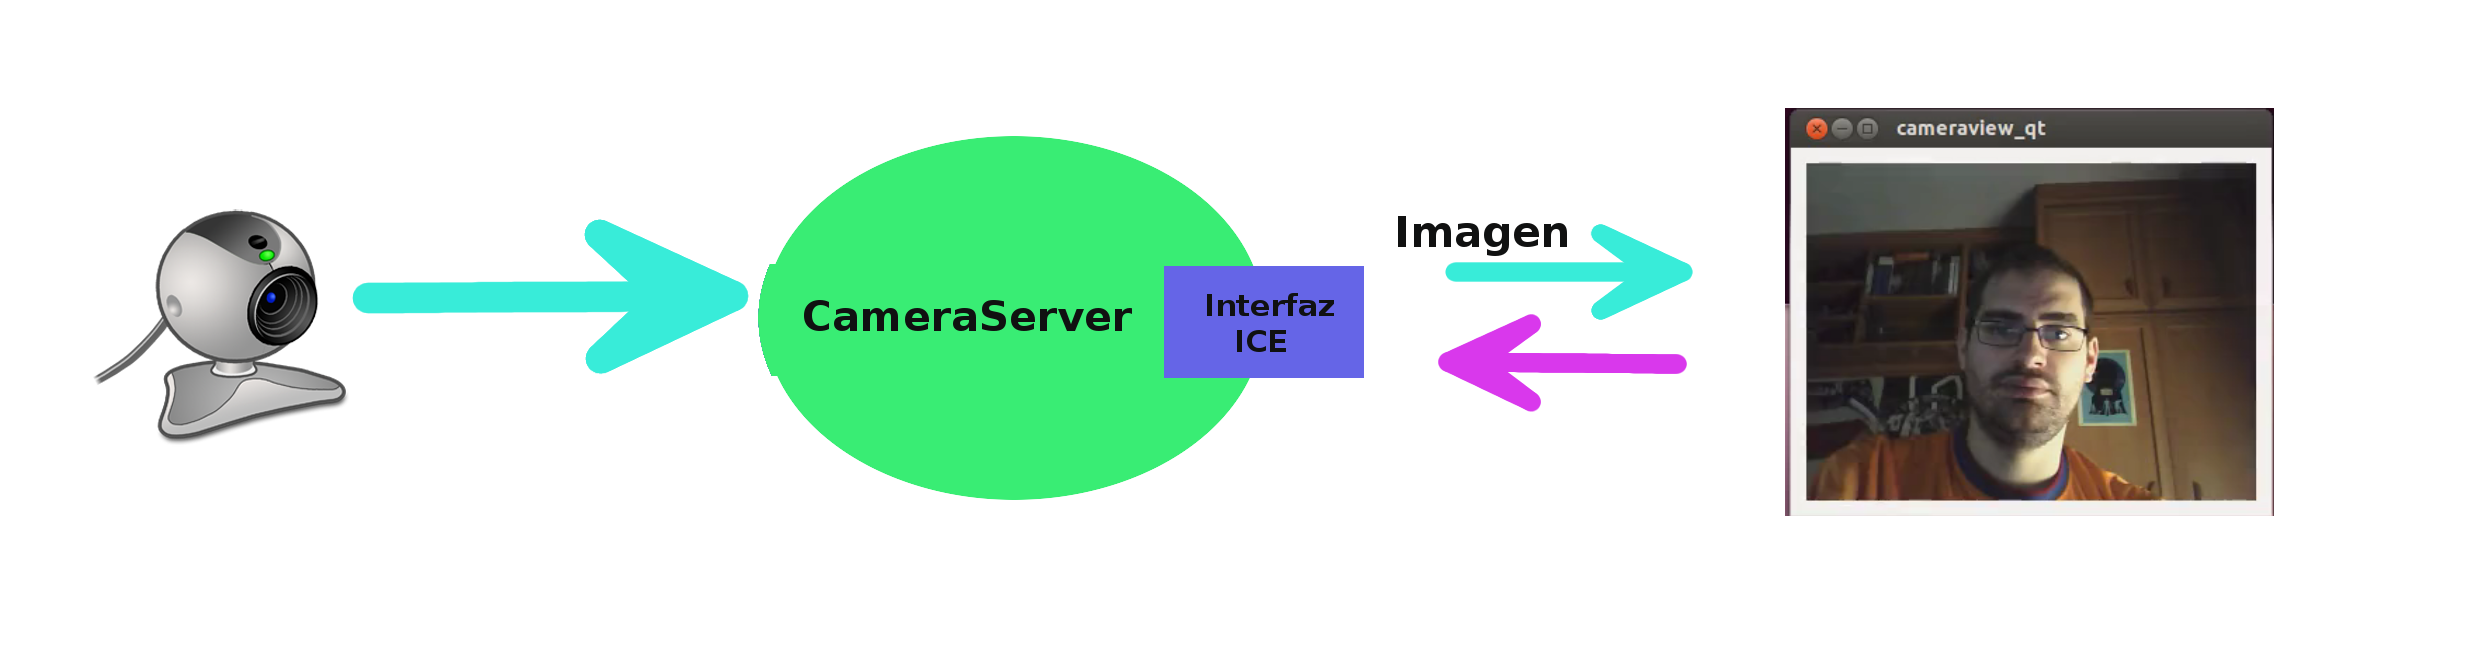
\includegraphics[width=0.8\textwidth]{./img/esq_cameraserver.png}
\caption{Ejemplo del uso del componente CameraServer.} \label{fig:esq_cameraserver}
\end{figure}

Cualquier programa que quiera conectarse con el componente \texttt{cameraserver} debe
importar la interfaz \texttt{camera.ice}. Esta interfaz a su vez importa otra llamada \texttt{image.ice}.
Esta �ltima contiene un m�todo llamado ``getImageData(String ImgFormat)''. Al invocar este m�todo se devuelve
una estructura formada por una imagen en el formato indicado con \texttt{ImgFormat} y las caracter�sticas de la misma.

Para la ejecuci�n de este componente, es necesario proporcionar la ruta de su archivo
de configuraci�n. En este fichero de configuraci�n se define la IP y puerto donde escucha
el servidor, el n�mero y nombre de las c�maras que tiene y la configuraci�n de las mismas.

\subsection{Openni1Server + RgbdViewer}

\texttt{Openni1Server}\cite {openni1server} es otro componente incluido en JdeRobot. Est� escrito en C++
y para su funcionamiento usa las librer�as Opencv\footnote{\url{http://opencv.org/}} y Openni\footnote{\url{http://www.openni.tk/openni/}} entre otras. Este
componente tiene todos los drivers necesarios para acceder al sensor Kinect y ofrece tres
tipos de datos: una imagen RGB, una imagen de profundidad y una nube de puntos. Al
ofrecer tres tipos distintos de datos tiene tres interfaces ICE. En este TFG s�lo se va a
hacer uso de las interfaces de im�genes. 

Para usar tanto la interfaz de imagen RGB como la de profundidad hacen falta los mismos interfaces ICE que en \texttt{CameraServer} ya que al 
tratarse de \textit{streamings} de im�genes se ha unificado la interfaz. De nuevo la interfaz contiene un m�todo llamado ``getImageData(String ImgFormat)''. Al invocar este m�todo se devuelve
una estructura formada por una imagen en el formato indicado con \texttt{ImgFormat} y las caracter�sticas de la misma, en el caso de la imagen RGB ImgFormat es ``RGB8'' 
mientras que en la imagen de distancia es ``DEPTH8\_16''. En la figura \ref{fig:esq_openniserver} se refleja �ste funcionamiento.

\begin{figure}[htb]
\centering
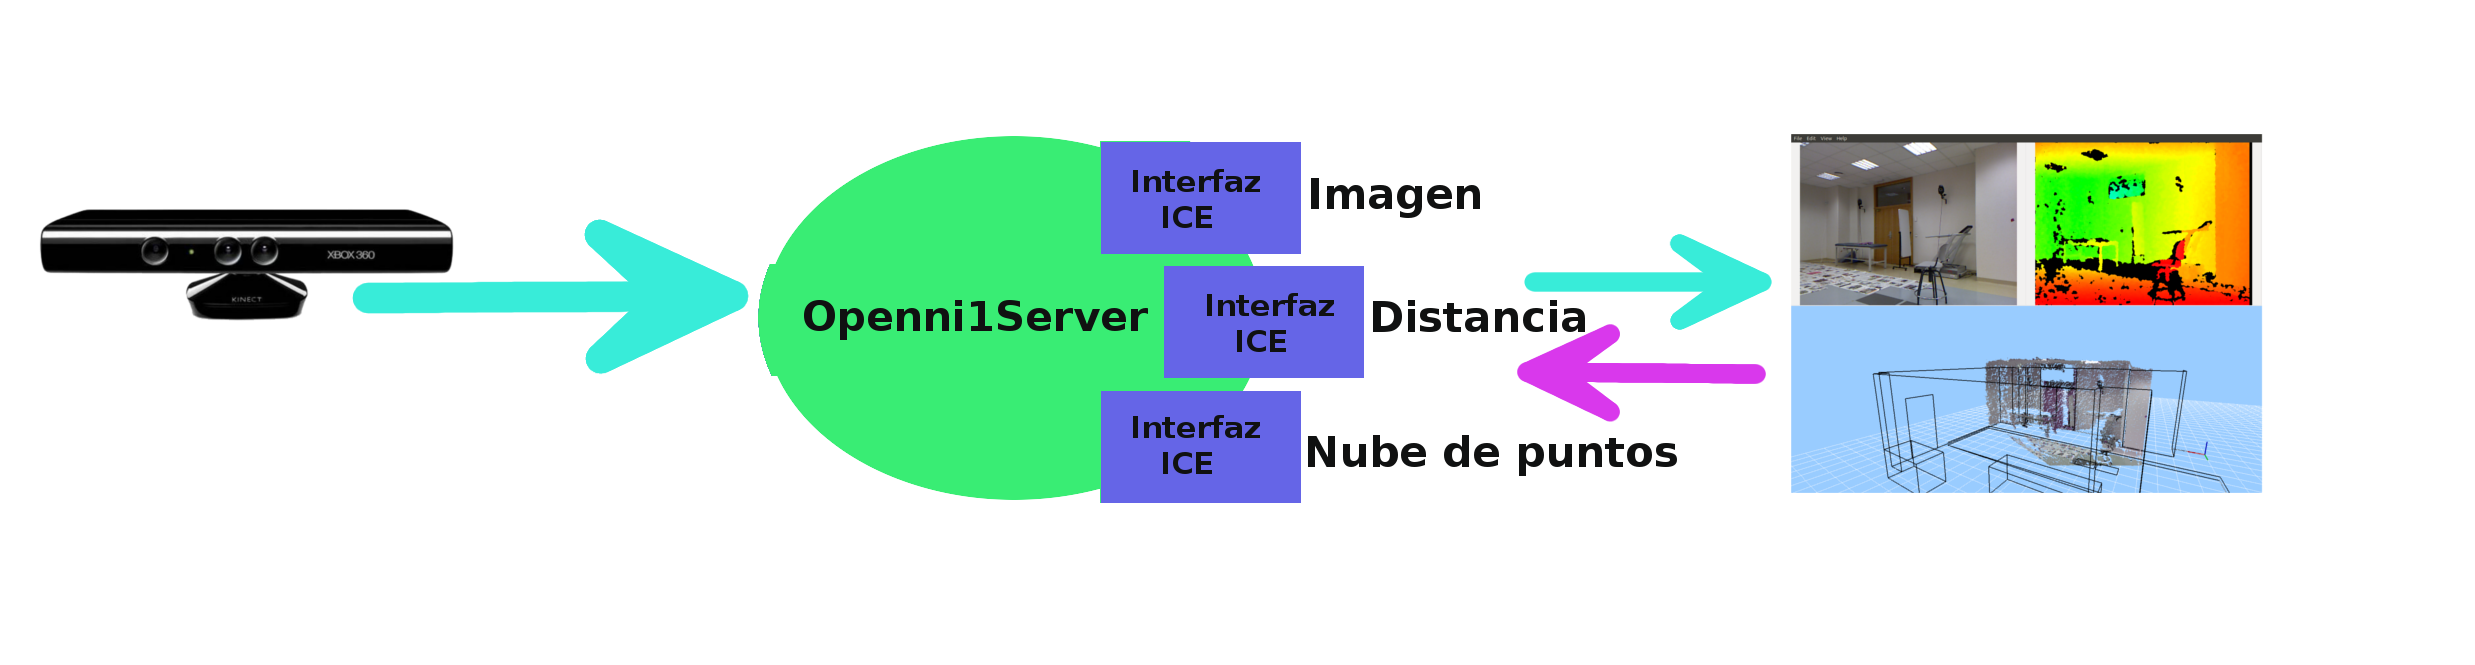
\includegraphics[width=1\textwidth]{./img/esq_openni1server.png}
\caption{Ejemplo del uso del componente Openni1Server.} \label{fig:esq_openniserver}
\end{figure}

\subsection{Ardrone\_server + uav\_viewer}

\texttt{Ardrone\_server}\cite {ardrone_server} es otro componente incluido en JdeRobot, escrito en C++. Este
componente permite comunicarse con el drone ArDrone 2 + GPS de Parrot, ofreciendo varias interfaces tanto para recibir informaci�n como para enviar �rdenes (Imagen, Pose3D, CmdVel, ...). 

Primero se enciende el drone, se conecta la m�quina a la red wifi suya y se ejecuta \texttt{Ardrone\_server}. A trav�s de
sus interfaces, el cliente recibe tanto la informaci�n de la imagen (misma interfaz que \texttt{cameraserver}), como el Pose3D (posici�n y orientaci�n del drone) 
y otras informaciones como pueden ser la bater�a restante por ejemplo (NavData). Tambi�n se pueden enviar �rdenes como 
la velocidad (CmdVel) u otras propias de aeronaves como despegar, aterrizar,...(ArDroneExtra).  
En la figura \ref{fig:esq_drone_server} se refleja �ste funcionamiento.

\begin{figure}[htb]
\centering
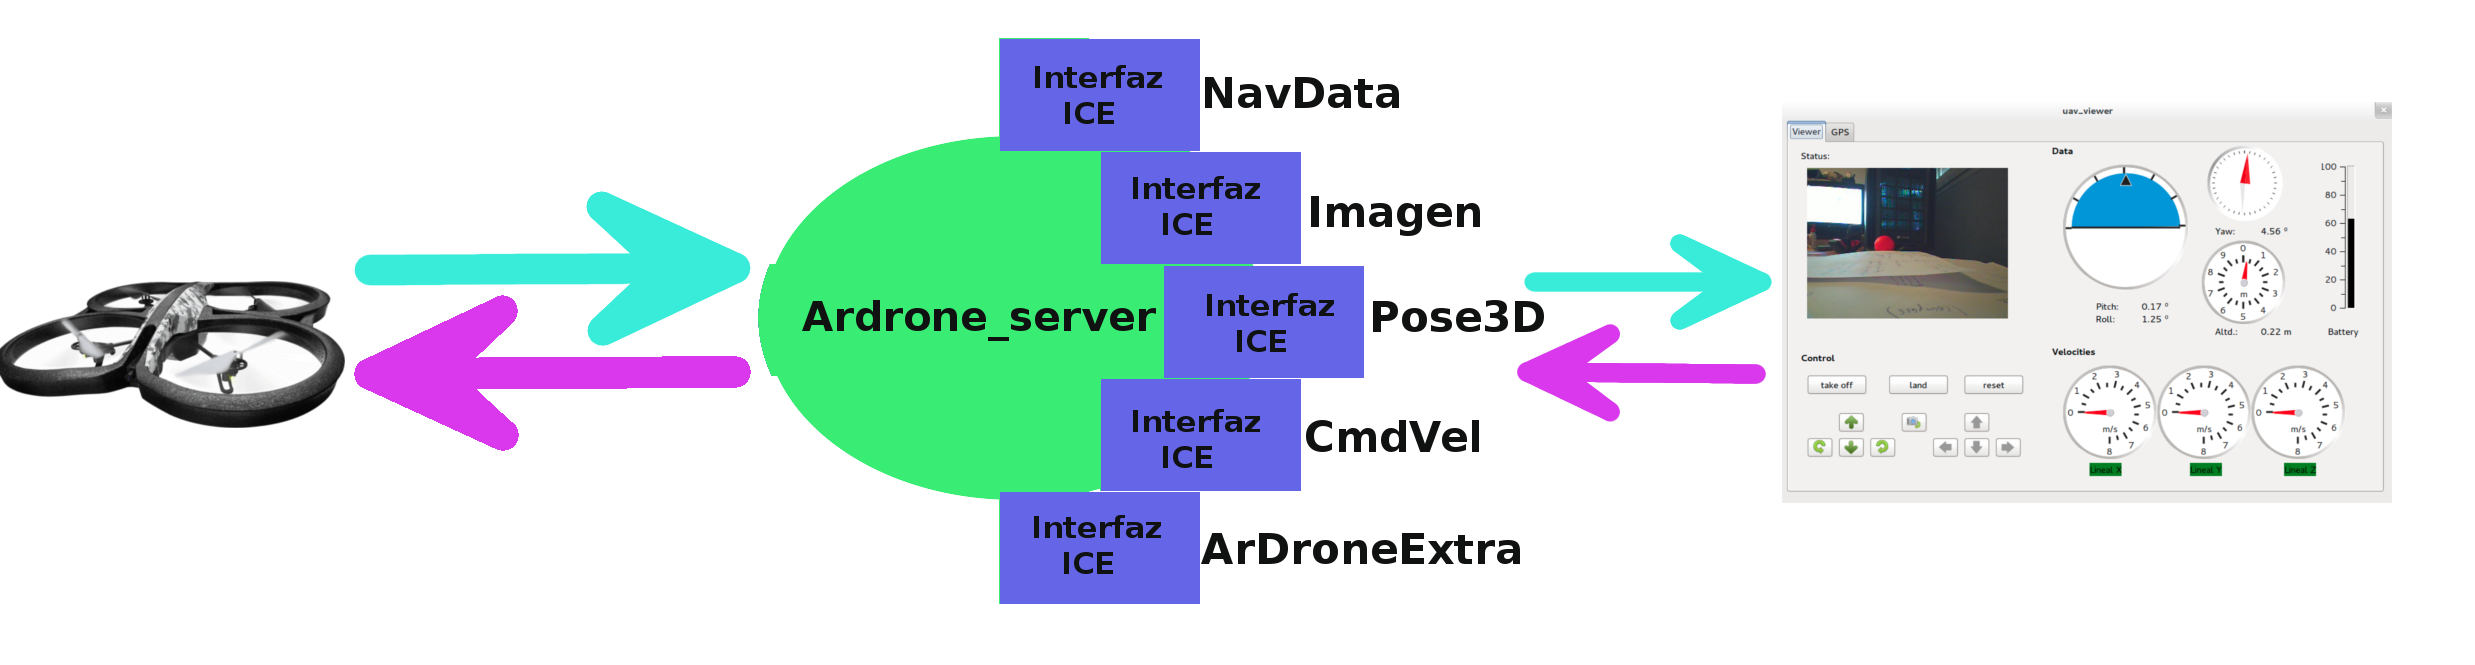
\includegraphics[width=1\textwidth]{./img/esq_drone_server.png}
\caption{Ejemplo del uso del componente Ardrone\_server.} \label{fig:esq_drone_server}
\end{figure}

\subsection{Kobuki\_driver + kobukiViewer}

\texttt{Kobuki\_driver}\cite {kobuki_driver} es otro componente incluido en JdeRobot, escrito en C++. Este
componente permite comunicarse con el robot Kobuki, ofreciendo varias interfaces tanto para recibir informaci�n como para enviar �rdenes (Imagen, Pose3D, Motors, ...). 

Primero se enciende el Kobuki, se conecta el robot por USB al PC y se ejecuta \texttt{kobuki\_driver}. A trav�s de
sus interfaces, el cliente recibe tanto la informaci�n de la imagen (misma interfaz que \texttt{cameraserver}), como el Pose3D (posici�n y orientaci�n del robot) 
y otras informaciones como pueden ser el l�ser por ejemplo (Laser). Tambi�n se pueden enviar �rdenes como 
la velocidad (Motors). En la figura \ref{fig:esq_kobuki} se refleja este funcionamiento.

\begin{figure}[htb]
\centering
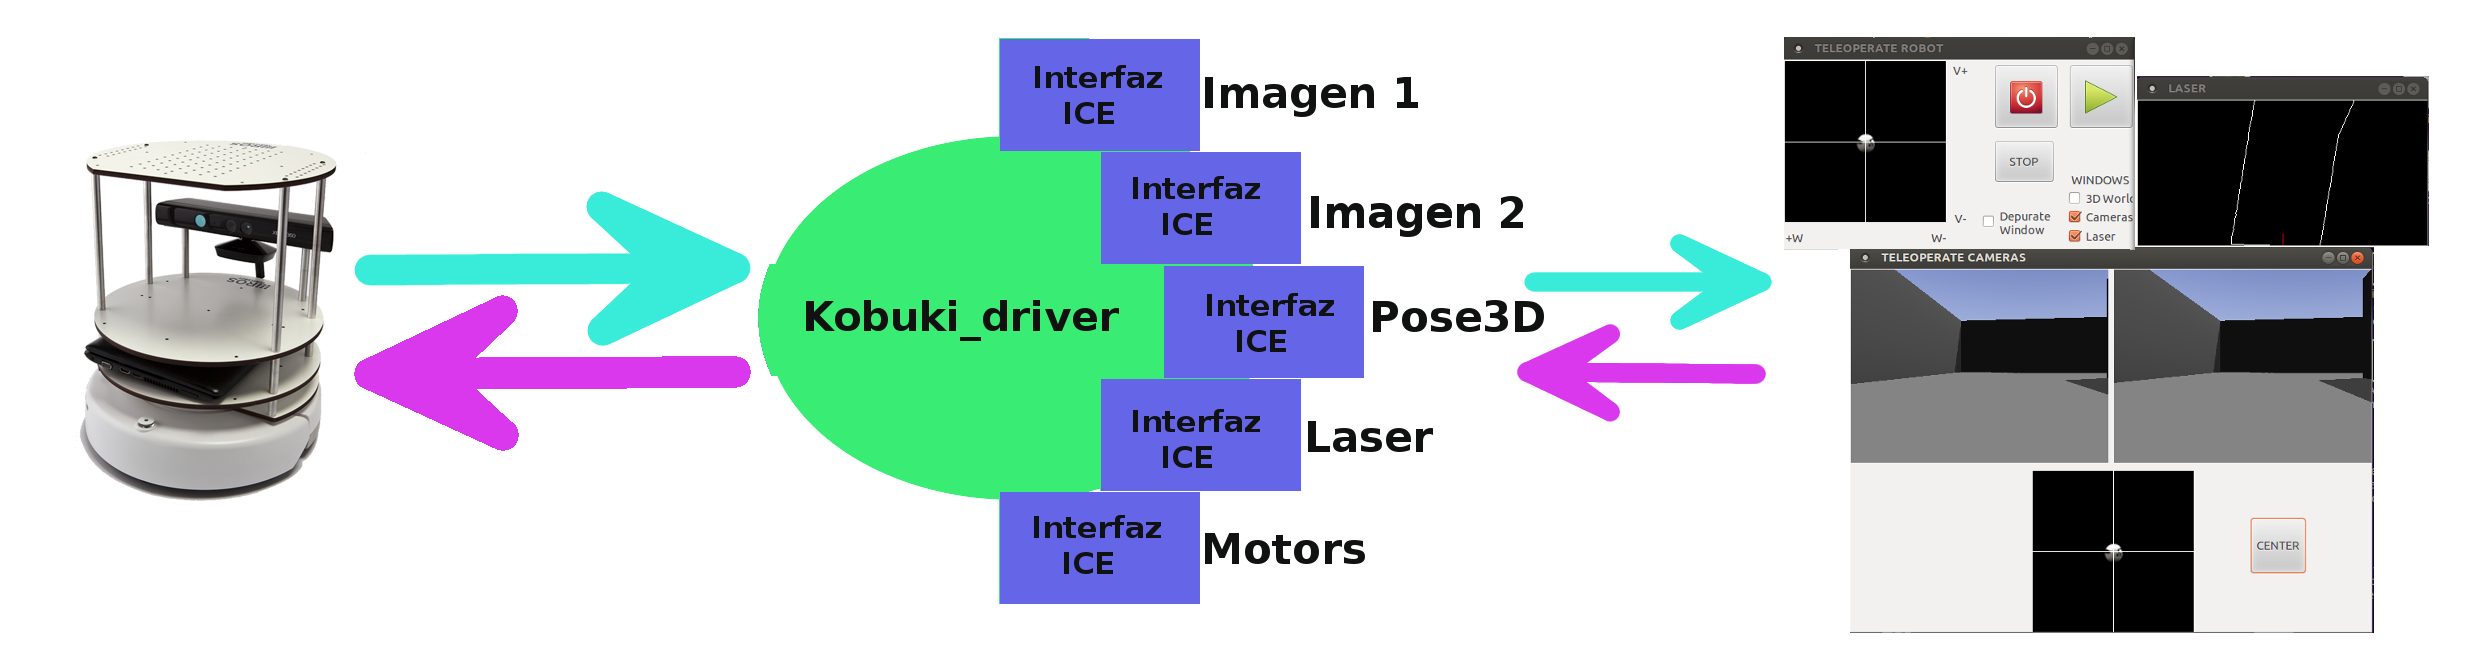
\includegraphics[width=1\textwidth]{./img/esq_kobuki.png}
\caption{Ejemplo del uso del Kobuki.} \label{fig:esq_kobuki}
\end{figure}


\section{HTML5}

HTML5\cite {html5} (HyperText Markup Language, versi�n 5) es la quinta revisi�n importante del lenguaje b�sico de la \textit{World Wide Web}, HTML. HTML5 especifica dos variantes de sintaxis para HTML: 
una �cl�sica�, HTML (text/html), conocida como HTML5, y una variante XHTML conocida como sintaxis XHTML5 que deber� servirse con sintaxis XML (application/xhtml+xml).
Esta es la primera vez que HTML y XHTML se han desarrollado en paralelo. La versi�n definitiva de la quinta revisi�n del est�ndar se public� en octubre de 2014\footnote{Est�ndar: \url{http://www.w3.org/TR/html5/}}.

HTML5 establece una serie de nuevos elementos y atributos que reflejan el uso t�pico de los sitios web modernos.
El desarrollo de este lenguaje de marcado es regulado por el Consorcio W3C\footnote{web de W3C: \url{http://www.w3.org/}}.

Algunos de los nuevos elementos introducidos son: \texttt{video} (permite reproducir v�deos sin la necesidad de \textit{plugins Flash}), \texttt{canvas} (Puede usarse para dibujar gr�ficos a trav�s JavaScript), 
\texttt{header} (representa la cabecera de la web, donde normalmente est� el men�), 
\texttt{progress} (permite mostrar una barra de progreso). En el siguiente c�digo se puede ver la etiqueta v�deo necesaria para el v�deo representado en la figura \ref{fig:htmlvideo}
\lstset{language=html}
\begin{lstlisting}
 <video style="width: 640px; height: 360px; left: 0px; top: 0px; transform: none;" class="video-stream html5-main-video" src="mediasource:https://www.youtube.com/54e5cca1-7aef-4865-ae1b-baab9047b526"></video>
\end{lstlisting}

\begin{figure}[htb]
\centering
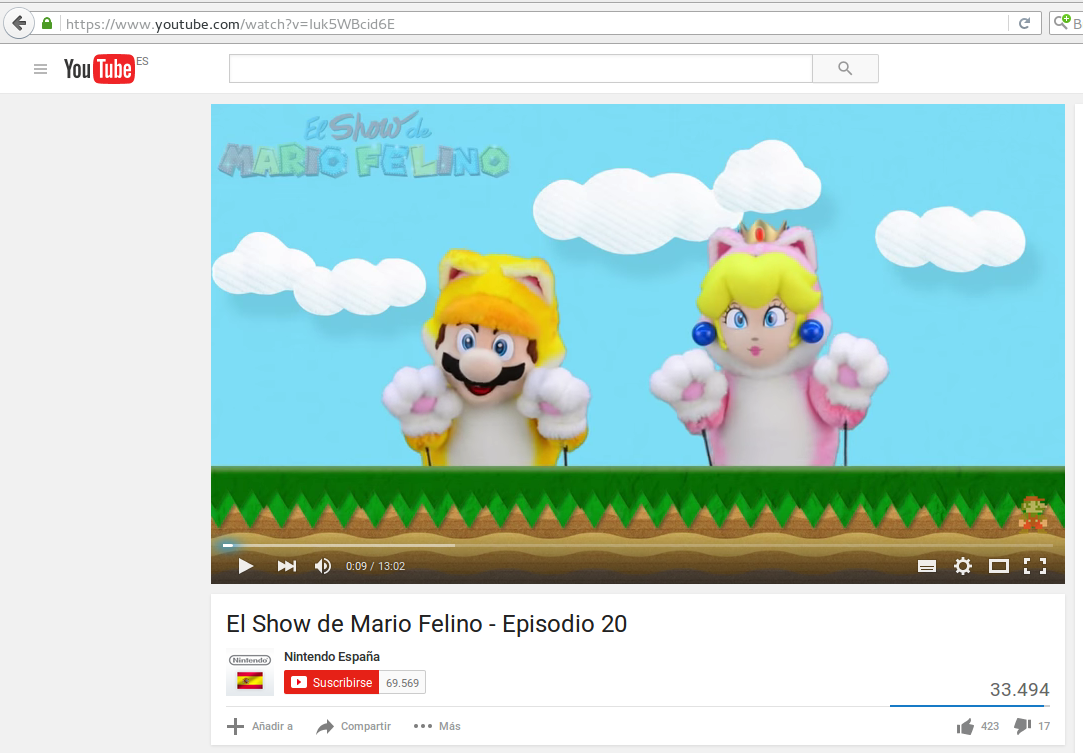
\includegraphics[width=0.8\textwidth]{./img/htmlvideo.png}
\caption{V�deo en Youtube.} \label{fig:htmlvideo}
\end{figure}

Nosotros usamos varios ingredientes asociados a HTML5 como son: \texttt{Canvas, WebWorkers y WebSockets}.
\subsection{Canvas}
 Consiste en una regi�n dibujable definida en el c�digo HTML con atributos de altura y ancho. El c�digo JavaScript puede acceder a la zona a 
 trav�s de un conjunto completo de funciones similares a las de otras APIs comunes de dibujo 2D, 
 permitiendo as� que los gr�ficos sean generados din�micamente. Algunos de los usos previstos incluyen construcci�n de gr�ficos, animaciones, juegos, y la composici�n de im�genes.
 
 Canvas fue introducido inicialmente por Apple para su uso dentro de su propio componente de Mac OS X surgido en 2004, para empujar aplicaciones como \textit{widgets} de \textit{Dashboard} y 
 el navegador Safari. M�s tarde, en 2005, se adopt� en la versi�n 1.8 de los navegadores Firefox y �pera en 2006. Fue estandarizado por el Grupo de Trabajo de Tecnolog�a de Aplicaci�n de hipertexto Web\footnote{web de WHATWG: \url{https://whatwg.org/}} 
 (WHATWG) sobre las nuevas especificaciones propuestas para tecnolog�as web de �ltima generaci�n. En la tabla \ref{tab:canvassupport} se puede ver desde qu� versi�n de los diferentes navegadores se soporta Canvas.
 
 \begin{table}[]
\centering
\label{tab:canvassupport}
\begin{tabular}{|l|l|l|c|l|l|c|c|c|}
\hline
\rowcolor{gray} 
{\color{White} IE} & {\color{White} Edge} & {\color{White} Firefox} & {\color{White} Chrome} & {\color{White} Safari} & {\color{White} Opera} & {\color{White} IOS Safari} & {\color{White} \begin{tabular}[c]{@{}c@{}}Android\\ Browser\end{tabular}} & {\color{White} \begin{tabular}[c]{@{}c@{}}Chrome\\ For Android\end{tabular}} \\ \hline
9                         & 12                          & 3.6                            & 4                             & 4                             & 10.1                         & 3.2                               & 3                                                                                & 7                                                                                   \\ \hline
\end{tabular}
\caption{Soporte de Canvas}
\end{table}

Nosotros lo utilizamos tanto para visualizar las im�genes recibidas de las c�maras como para mostrar los modelos 3D de los robots.
\subsection{WebWorker}

Uno de los mayores problemas que tienen las aplicaciones web es que JavaScript es un entorno de subproceso �nico, es decir, que no se pueden ejecutar varias secuencias de comandos al mismo tiempo. 
Los desarrolladores imitaban la ``simultaneidad'' utilizando t�cnicas como \texttt{setTimeout()} o \texttt{setInterval()} que lo �nico que hacen es programas la ejecuci�n de una funci�n, pero se sigue ejecutando s�lo una funci�n cada vez.


Los \textbf{WebWorkers} proveen un medio sencillo para que el contenido web ejecute \textit{scripts} en hilos en segundo plano. El hilo \textit{worker} puede realizar tareas sin interferir con la interfaz de usuario. 
No tienen acceso al DOM (Document Object Model es un conjunto de utilidades dise�adas para manipular documentos HTML de forma r�pida y eficiente) ni a otras zonas sensibles para evitar problemas de concurrencia (en la figura  \ref{fig:webworker} se pueden ver los elementos a los que tiene acceso cada hilo), por lo que el intercambios de informaci�n entre \textit{Worker} e hilo principal se hace mediante paso de mensajes.

\begin{figure}[htb]
\centering
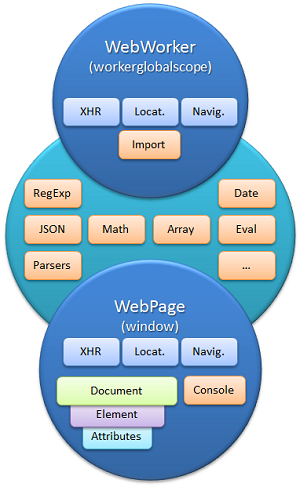
\includegraphics[width=0.3\textwidth]{../traspas/img/worker.png}
\caption{Elementos WebWorker.} \label{fig:webworker}
\end{figure}

En la tabla \ref{tab:workersupport} se puede ver desde qu� versi�n de los diferentes navegadores se soporta WebWorker.

 \begin{table}[]
\centering
\label{tab:workersupport}
\begin{tabular}{|l|l|l|c|l|l|c|c|c|}
\hline
\rowcolor{gray} 
{\color{White} IE} & {\color{White} Edge} & {\color{White} Firefox} & {\color{White} Chrome} & {\color{White} Safari} & {\color{White} Opera} & {\color{White} IOS Safari} & {\color{White} \begin{tabular}[c]{@{}c@{}}Android\\ Browser\end{tabular}} & {\color{White} \begin{tabular}[c]{@{}c@{}}Chrome\\ For Android\end{tabular}} \\ \hline
10                         & 12                          & 3.5                            & 4                             & 4                             & 11.5                         & 5.1                               & 4.4                                                                                & 47                                                                                   \\ \hline
\end{tabular}
\caption{Soporte para WebWorker}
\end{table}
\subsection{WebSocket}
\texttt{WebSocket} es una tecnolog�a que proporciona un canal de comunicaci�n bidireccional y \textit{full-duplex} sobre un �nico \textit{socket} TCP. 
Est� dise�ada para ser implementada en navegadores y servidores web, pero puede utilizarse por cualquier aplicaci�n cliente/servidor. 
La API de \textit{WebSocket} est� siendo normalizada por el W3C\footnote{\url{http://www.w3.org}}. Debido a que las conexiones TCP comunes sobre puertos diferentes al 80 son 
habitualmente bloqueadas por los administradores de redes, el uso de esta tecnolog�a proporcionar�a una soluci�n a este tipo de limitaciones 
proveyendo una funcionalidad similar a la apertura de varias conexiones en distintos puertos, pero multiplexando diferentes servicios \textit{WebSocket} 
sobre un �nico puerto TCP (a costa de una peque�a sobrecarga del protocolo).

En la tabla \ref{tab:socketsupport} se puede ver desde qu� versi�n de los diferentes navegadores se soporta WebWorker.
 \begin{table}[]
\centering
\label{tab:socketsupport}
\begin{tabular}{|l|l|l|c|l|l|c|c|c|}
\hline
\rowcolor{gray} 
{\color{White} IE} & {\color{White} Edge} & {\color{White} Firefox} & {\color{White} Chrome} & {\color{White} Safari} & {\color{White} Opera} & {\color{White} IOS Safari} & {\color{White} \begin{tabular}[c]{@{}c@{}}Android\\ Browser\end{tabular}} & {\color{White} \begin{tabular}[c]{@{}c@{}}Chrome\\ For Android\end{tabular}} \\ \hline
10                         & 12                          & 11                            & 16                             & 7                             & 12.1                         & 6.1                               & 4.4                                                                                & 47                                                                                   \\ \hline
\end{tabular}
\caption{Soporte para WebSocket}
\end{table}
\section{CSS3}

Hoja de estilo en cascada o CSS (\textit{cascading style sheets}) es un lenguaje usado para definir y crear la presentaci�n de un documento estructurado escrito en HTML. El \textit{World Wide Web Consortium}\footnote{web de W3C: \url{http://www.w3.org/}} 
es el encargado de formular la especificaci�n de las hojas de estilo que servir�n de est�ndar para los agentes de usuario o navegadores.

La idea que se encuentra detr�s del desarrollo de CSS es separar la estructura de un documento de su presentaci�n. La informaci�n de estilo puede ser definida 
en un documento separado o en el mismo documento HTML. En este �ltimo caso podr�an definirse estilos generales con el elemento �style� o en cada etiqueta particular mediante el atributo �style�.

CSS tiene una sintaxis muy sencilla, que usa unas cuantas palabras clave tomadas del ingl�s para especificar los nombres de varias propiedades de estilo, por ejemplo, \textit{width} o \textit{bottom-padding}.

A diferencia de las versiones anteriores, CSS3 est� dividida en varios documentos separados, llamados ``m�dulos''. 
Cada m�dulo a�ade nuevas funcionalidades a las definidas en CSS2, de manera que se preservan las anteriores para mantener la compatibilidad.

Nosotros lo usamos para modificar la apariencia de la p�gina web a nuestro gusto.

\section{JavaScript6}

JavaScript6 o ECMAScript 2015 es la versi�n actual de la especificaci�n del lenguaje ECMAScript conocida simplemente como ``ES6''.

Agrega cambios significativos en la sintaxis para escribir aplicaciones complejas, incluyendo clases y m�dulos, defini�ndolos s�manticamente en 
los mismos t�rminos del modo estricto de la edici�n ECMAScript 5. Otras nuevas caracter�sticas incluyen iteradores \texttt{for/of loops}, generadores
expresiones estilo Python, funciones de direcci�n, datos binarios, colecciones (mapas, sets, mapas d�biles) y \textit{proxies} (metaprogramaci�n para objetos virtuales y \textit{wrappers}). 

El nuevo ingrediente de JavaScript6 que se utiliza en este TFG es el objeto \textit{Promise}, que devuelve una promesa de tener un valor en alg�n momento en el futuro.

\subsection{Promise}

La interfaz \textit{Promise} representa un \textit{proxy} para un valor no necesariamente conocido cuando se crea la promesa. Permite asociar manejadores a un eventual �xito o 
fracaso de acciones as�ncronas. Esto permite que los m�todos as�ncronos devuelven valores como m�todos s�ncronos: en lugar del valor final, el m�todo as�ncrono 
devuelve una promesa de tener un valor en alg�n momento en el futuro.

Una Promesa puede estar en uno de estos estados:
\begin{itemize}
 \item \textit{Pending}: estado inicial, no cumplida o rechazada.
 \item \textit{Fulfilled}: operaci�n satisfactoria.
 \item \textit{Rejected}: operaci�n fallida.
\end{itemize}

Una promesa pendiente puede llegar a ser cumplida con un valor o rechazada con una raz�n. Cuando cualquiera de ellas sucede, los manejadores asociados 
se llaman mediante el m�todo \texttt{then} de la promesa. (Si la promesa ya se ha cumplido o rechazado cuando se conecta un controlador correspondiente, el manejador ser� llamado, 
as� que no hay condici�n de competencia entre el final de una operaci�n as�ncrona y sus manejadores). En la figura \ref{fig:promise} pueden los estados y como se pasa a ellos.

\begin{figure}[htb]
\centering
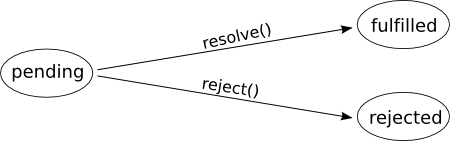
\includegraphics[width=0.8\textwidth]{../traspas/img/promise-tilstande1.png}
\caption{Vida de una Promise} \label{fig:promise}
\end{figure}

En la tabla \ref{tab:pormisesupport} se puede ver desde qu� versi�n de los diferentes navegadores se soporta Promise.

 \begin{table}[]
\centering
\label{tab:pormisesupport}
\begin{tabular}{|l|l|l|c|l|l|c|c|c|}
\hline
\rowcolor{gray} 
{\color{White} IE} & {\color{White} Edge} & {\color{White} Firefox} & {\color{White} Chrome} & {\color{White} Safari} & {\color{White} Opera} & {\color{White} IOS Safari} & {\color{White} \begin{tabular}[c]{@{}c@{}}Android\\ Browser\end{tabular}} & {\color{White} \begin{tabular}[c]{@{}c@{}}Chrome\\ For Android\end{tabular}} \\ \hline
no soportado                         & 12                          & 29                            & 33                             & 7.1                             & 20                         & 8                               & 4.4.4                                                                                & 47                                                                                   \\ \hline
\end{tabular}
\caption{Soporte para Promise}
\end{table}

\section{WebGL}

WebGL\cite{webgl} es una especificaci�n est�ndar, basada en OpenGL ES 2.0, que est� siendo desarrollada actualmente para mostrar gr�ficos en 3D en navegadores web. 
Permite mostrar gr�ficos en 3D acelerados por hardware (GPU) en p�ginas web, sin la necesidad de \textit{plugins} en cualquier plataforma que soporte OpenGL 2.0 u OpenGL ES 2.0.

WebGL carece de las rutinas matem�ticas matriz eliminadas en OpenGL 3.0. Esta funcionalidad debe ser proporcionada por el usuario; 
este c�digo necesario se complementa con frecuencia con una biblioteca de matrices tal como glMatrix, TDL, o MJS.

Como WebGL es una tecnolog�a dise�ada para trabajar directamente con la GPU (unidad de procesamiento gr�fico) es dif�cil de codificar en comparaci�n con otros est�ndares web m�s accesibles, 
por lo que ha surgido muchas bibliotecas JavaScript para resolver este problema:  Curve3D, CubicVR, EnergizeGL, O3D,  TDL, Three.js, X3DOM. BabylonJS...

Las m�s destacadas son Three.js,  que es la m�s usada y con la que se trabaja en este proyecto, y BabylonJS que est� desarrollada por Microsoft.

\begin{figure}[htb]
\centering
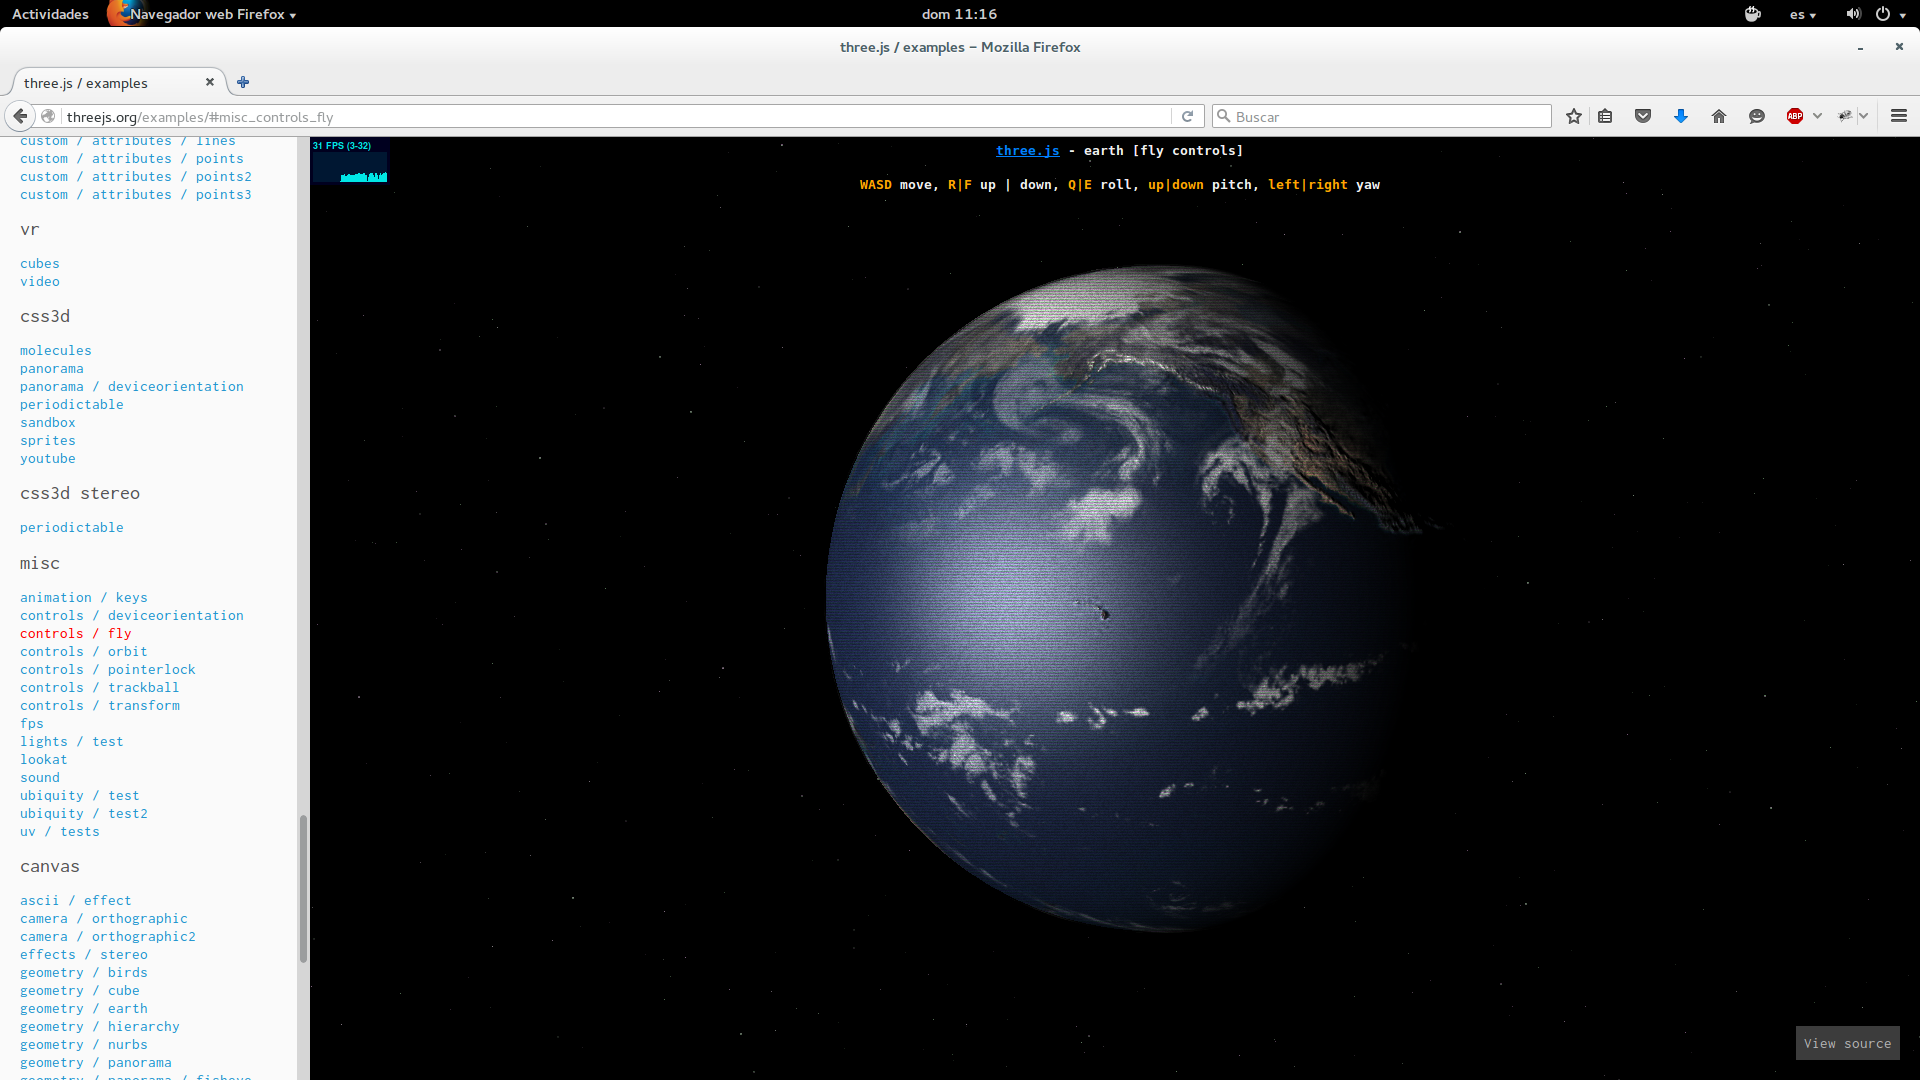
\includegraphics[width=0.7\textwidth]{../traspas/img/canvas2.png}
\caption{Ejemplo mundo WebGl con Three.js.} \label{fig:webgl}
\end{figure}

Nosotros la usamos para crear los modelos 3D de los robots.
\section{ThreeJS}

Three.js\cite{threejs} es una biblioteca escrita en JavaScript para crear y mostrar gr�ficos animados por ordenador en 3D en un navegador Web 
y puede ser utilizada en conjunci�n con el elemento canvas de HTML5, SVG � WebGL. Es la m�s usada para crear animaciones con WebGL (figura \ref{fig:webgl}).

Caracter�sticas:
\begin{itemize}
\item Renderizadores: Canvas, SVG y WebGL.
\item Efectos: anaglifo, bizco y la barrera de paralaje.
\item Escenas: a�adir y eliminar objetos en tiempo de ejecuci�n; niebla.
\item C�maras: perspectiva y ortogr�fica; controladores: trackball, FPS, trayectoria y otras.
\item Animaci�n: armaduras, cinem�tica directa, cinem�tica inversa,\textit{ morphing} y fotogramas clave.
\item Luces: ambiente, direcci�n, luz de puntos y espacios, sombras: emite y recibe.
\item Materiales: Lambert, Phong, sombreado suave, texturas y otras.
\item Shaders: el acceso a las capacidades del OpenGL \textit{Shading Language} (GLSL): reflejos en la lente, pase profundo y una extensa biblioteca de post-procesamiento
\item Objetos: mallas, part�culas, \textit{sprites}, l�neas, cintas, huesos y otros.
\item Geometr�a: plano, cubo, esfera, toroide, texto en 3D y otras; modificadores: torno, extrusi�n y tubo.
\item Cargadores de datos: binario, imagen, JSON y escena.
\item Utilidades: conjunto completo de funciones matem�ticas en 3D, incluyendo tronco, matriz Quaternian, UVs y otras.
\end{itemize}

Incluso est�n a�adiendo funciones para realidad virtual.

Nosotros la usamos para facilitar el acceso a WebGL.
\section{JQuery}

jQuery\cite{jquery} es una biblioteca de JavaScript que permite simplificar la manera de interactuar con los documentos HTML, manipular el �rbol DOM, manejar eventos, desarrollar animaciones y agregar interacci�n con la t�cnica AJAX a p�ginas web. 

Es la biblioteca de JavaScript m�s utilizada y ofrece una serie de funcionalidades que de otra manera requerir�an de mucho m�s c�digo por lo que se ahorra tiempo y espacio.

Caracter�sticas:
\begin{itemize}
\item Selecci�n de elementos DOM.
\item Interactividad y modificaciones del �rbol DOM, incluyendo soporte para CSS 1-3 y un \textit{plugin} b�sico de XPath.
\item Eventos.
\item Manipulaci�n de la hoja de estilos CSS.
\item Efectos y animaciones.
\item Animaciones personalizadas.
\item AJAX.
\item Soporta extensiones.
\item Utilidades varias como obtener informaci�n del navegador, operar con objetos y vectores, funciones para rutinas comunes, etc.
\item Compatible con los navegadores Mozilla Firefox 2.0+, Internet Explorer 6+, Safari 3+, Opera 10.6+ y Google Chrome 8+.

La versi�n utilizada en el proyecto es la 1.11.3.
\end{itemize}

En la tabla \ref{tab:jquery} se puede ver una comparativa entre JQuery y los m�todos por defecto de JavaScript.

\begin{table}[]
\centering
\begin{tabular}{|l|l|}
\hline
\rowcolor{gray} 
\multicolumn{1}{|c|}{\color{White} JQuery}                                                                 & \multicolumn{1}{c|}{ \color{White} JavaScript}                                                                                                                                                                 \\ \hline
var divs = \$(``div'');                                                                        & var divs = document.querySelectorAll (``div'');                                                                                                                                                   \\ \hline
var newDiv = \$(``$<$div/$>$'');                                                & var newDiv = document.createElement(``div'');                                                                                                                                                     \\ \hline
\begin{tabular}[c]{@{}l@{}}\$(``a'').click (function(\{\\    //code\\ \});\end{tabular}        & \begin{tabular}[c]{@{}l@{}}{[} {]}.forEach.call (document.querySelectorAll (``a''),function (el)\{  \\    el.addEventListener (``click'',function()\{\\       //code  \\    \});\\ \});\end{tabular} \\ \hline
\end{tabular}
\label{tab:jquery}
\caption{Comparaci�n JQuery, JavaScript}
\end{table}

\section{Bootstrap}

Bootstrap\cite{bootstrap} es un \textit{framework} o conjunto de herramientas de software libre para dise�o de sitios y aplicaciones web. 
Contiene plantillas de dise�o con tipograf�a, formularios, botones, cuadros, men�s de navegaci�n y otros elementos de dise�o 
basado en HTML y CSS, as� como extensiones de JavaScript opcionales adicionales.

Bootstrap fue desarrollado por Mark Otto y Jacbod Thornton de Twitter, como un marco de trabajo para fomentar la consistencia a trav�s de herramientas internas. 
Antes de Bootstrap, se usaban varias librer�as para el desarrollo de interfaces de usuario, las cuales guiaban a inconsistencias y a una carga de trabajo alta en su mantenimiento.

En agosto del 2011, Twitter liber� a Bootstrap como c�digo abierto. En febrero del 2012, se convirti� en el proyecto de desarrollo m�s popular de GitHub y es usado por la NASA (figura \ref{fig:nasa}), la universidad de Washington, la FIFA...

\begin{figure}[htb]
\centering
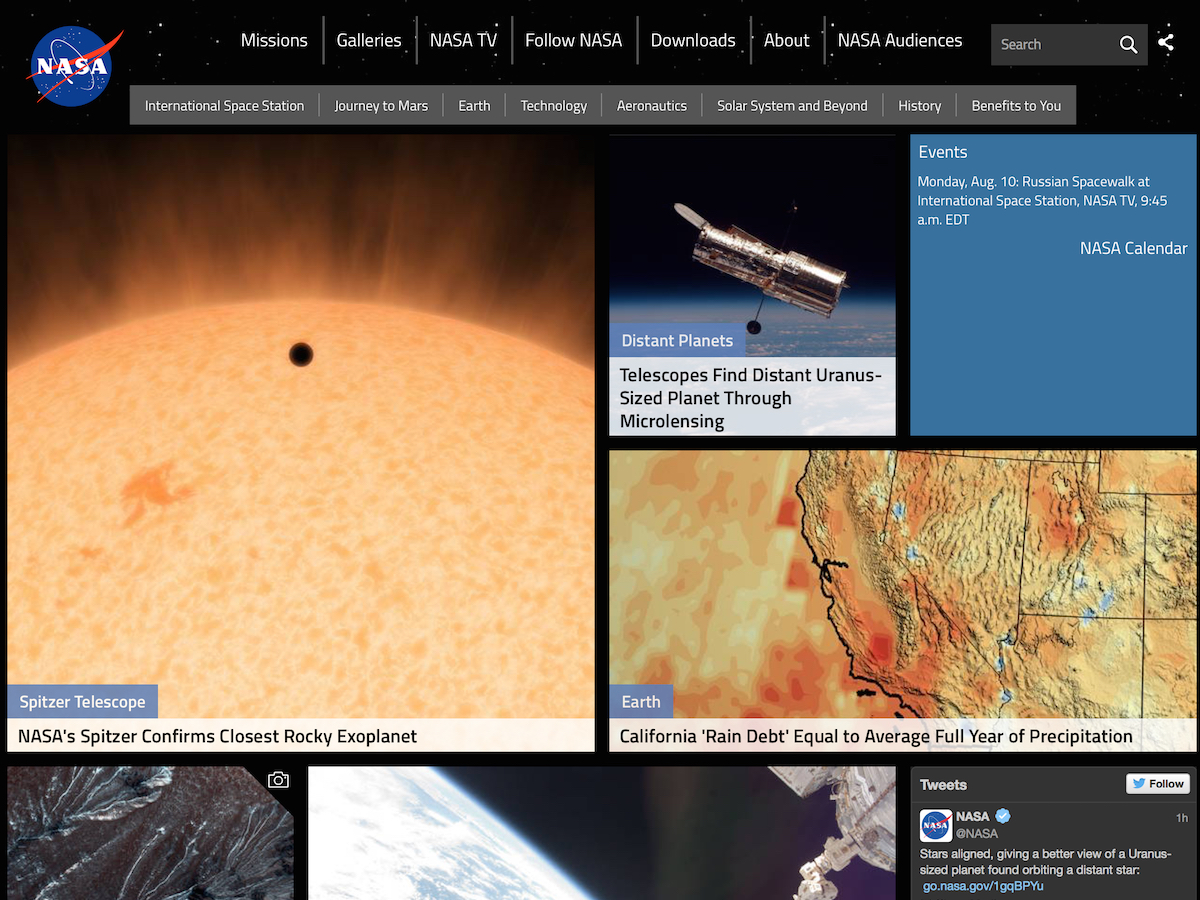
\includegraphics[width=0.7\textwidth]{./img/nasa.jpg}
\caption{Web de la NASA.} \label{fig:nasa}
\end{figure}

En este proyecto se usa la versi�n 3 para la maquetaci�n de la p�gina web.


\section{ICE for Javascript}

ICE for Javascript o Ice-JS\cite{icejs}, es una nueva implementaci�n de ICE adaptada para aplicaciones web que usan JavaScript. 
Como los navegadores web no pueden usar los protocolos comunes de ICE, sino que s�lo pueden usar \textit{websocket}\cite{icews}, 
incluye un \textit{plugin} para procesos en C++ que les permite usar este protocolo. Un esquema del funcionamiento de Ice-JS se encuentra en la figura \ref{fig:icejsapp}.

\begin{figure}[htb]
\centering
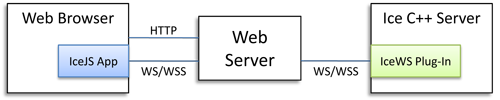
\includegraphics[width=0.8\textwidth]{./img/icejsapp.png}
\caption{Esquema de funcionamiento de Ice-JS.} \label{fig:icejsapp}
\end{figure}

En la versi�n 3.5 de ICE todav�a era una beta y estaba aparte\footnote{descarga de Ice-JS \url{https://zeroc.com/labs/icejs/download.html}}, 
pero ya en la 3.6 est� totalmente incluida en el paquete general de ICE. En este proyecto se usa la versi�n beta.










\chapter{Dise�o y programaci�n}
\label{ch:Diseno}

Una vez explicados en los cap�tulos anteriores los requisitos
y las herramientas necesarias para la elaboraci�n del proyecto, 
en este cap�tulo se va a explicar la soluci�n desarrollada al problema planteado en el cap�tulo objetivos. 
Se va a comenzar dando una visi�n general del
dise�o y posteriormente se describir�n sus detalles y la
implementaci�n de cada una de sus partes.

\section{Dise�o global} \label{sec:diseno-global}
 
El dise�o que se presenta se ha elegido porque cumple todos los objetivos
y requisitos expuestos en el cap�tulo 2. La arquitectura del sistema tiene dos partes
diferenciadas tal y como se observa en la figura \ref{fig:JdeRobotwebclients}: Servidores y clientes.

\begin{figure}[htb]
\centering
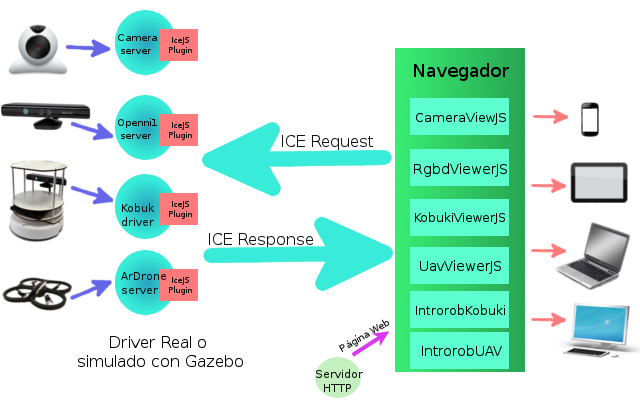
\includegraphics[width=0.9\textwidth]{../traspas/img/esq_proyecto.png}
\caption{Arquitectura de JdeRobotWebClients} \label{fig:JdeRobotwebclients}
\end{figure}

 \textbf{Servidores}. Se han utilizado 4 servidores distintos, dos de sensores (el de c�mara y el de Kinect) y dos de robots (Kobuki y Drone). 
 %el de Kinect (\texttt{Openni1Server}) y dos de robots completos, el de robots kobuki (\texttt{kobuki_driver})y el de un Drone (\texttt{ardrone_server}), 
 Estos dos �ltimos pueden ser reales o simulados mediante Gazebo.
 Cada uno de los servidores se corresponde con componentes de JdeRobot ya existentes a los que se les ha a�adido en la configuraci�n la ubicaci�n de un \textit{plugin} 
 para que puedan usar el protocolo \texttt{WebSockect}, necesario 
 para que los navegadores web puedan comunicarse con estos servidores. Este \textit{plugin} viene con la instalaci�n de Ice-JS. 
 Adem�s, todos los componentes involucrados usan una interfaz ICE para comunicarse y transmitir esos datos al servidor Web o a otros componentes. Esto 
 hace que cada componente pueda correr en una m�quina distinta.
 
 Los \textbf{clientes} est�n desarrollados mediante JavaScript, HTML y CSS. Para dotarlos de la mayor flexibilidad posible constan de 3 partes muy diferenciadas, 
 como puede verse en la figura \ref{fig:nivelesweb}: conexi�n con servidor, n�cleo e interfaz gr�fico.
 \begin{enumerate}
 \item Conector. Est� desarrollado �ntegramente en JavaScript. Se encarga de la comunicaci�n con el servidor de sensores o de robots. Permite crear la conexi�n y recibir los datos. Para ello primero crea un hilo separado 
 que es el que se conecta con el servidor ICE. Una vez creada la conexi�n, el hilo principal mediante RPC's indica a este segundo hilo los m�todos que debe ejecutar del servidor. Un cliente tiene tantos 
 conectores como interfaces ICE tenga el servidor. Para comunicarse con dicho servidor utilizan ICE-JS que est� escrito en JavaScript y permite utilizar interfaces ICE sobre el protocolo \texttt{WebSockect}.
 \item N�cleo. Esta parte est� desarrollada �ntegramente en JavaScript. Se encarga del funcionamiento interno de cada uno de los \textit{widgets} del cliente, ya sea mostrar los datos recibidos de los sensores
 o mandar los datos a los actuadores.
 \item Interfaz gr�fico. Engloba la parte HTML y CSS y algo de JavaScript de los clientes e indica c�mo se organizan cada uno de los \textit{widgets} del cliente dentro de la p�gina web.
 \end{enumerate}
 

 \begin{figure}[htb]
\centering
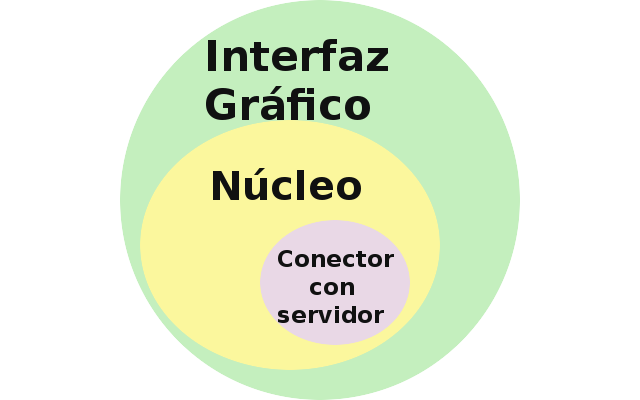
\includegraphics[width=0.4\textwidth]{./img/niveles_web.png}
\caption{Niveles de los clientes} \label{fig:nivelesweb}
\end{figure}

En total son 6 clientes: \texttt{CameraViewJS} (1), que recibe datos de \textit{CameraServer}; \texttt{RgbdViewerJS} (2), que recibe datos de \texttt{Openni1Server}; 
\texttt{KobukiViewerJS} (3), que permite teleoperar robots Kobuki; \texttt{UavViewerJS} (4), que permite teleoperar drones y los dos que adem�s de teleoperar dan soporte para crear 
comportamiento aut�nomo en los robots o drones, \texttt{IntrorobKobukiJS} (5) e \texttt{IntrorobUavJS} (6).

Adicionalmente, hemos creado una p�gina web, a modo de envoltorio �nico, que empotra en pesta�as los seis clientes desarrollados.


\subsection{Servidores} \label{sec:servidores}
En esta secci�n se describe el funcionamiento de los componentes de JdeRobot ya existentes usados en este TFG. Su funcionamiento general se ha detallado
en la secci�n \ref{sec:plat_jderobot}.
\texttt{Cameraserver} \cite {cameraserver} es el componente encargado de acceder a la c�mara web
para entregar v�a ICE las im�genes necesarias para \textit{streaming} de v�deo.
\texttt{Openni1Server} \cite {openni1server} es el componente necesario para acceder al sensor
Kinect. De este componente se obtienen las im�genes de profundidad. 
\texttt{Ardrone\_server} \cite {ardrone_server} es el componente necesario para acceder al drone. 
Hace de intermediario entre el drone y el cliente.
\texttt{Kobuki\_driver} \cite {kobuki_driver} es el componente necesario para acceder al Kobuki. 
Hace de intermediario entre el Kobuki y el cliente.

Se ha tenido que hacer variaciones en sus ficheros de configuraci�n para permitirles usar el protocolo \textit{websocket} ya que es el �nico 
que usan los Navegadores web. Para ello hay que indicarle en la configuraci�n que use el \textit{plugin} mediante la siguiente l�nea (No hace falta recompilar el c�digo fuente del propio servidor):
\lstset{language=Ruby}
\begin{lstlisting}
    # Ice-JS
    Ice.Plugin.IceWS=IceWS:createIceWS
\end{lstlisting}

Una vez hecho esto ya se le puede indicar que escuche en un puerto mediante el protocolo \textit{WebSokect} (ws) a�adiendo al \textit{endpoint}:
\begin{lstlisting}
    # Ice-JS
    :ws -h IP -p PUERTO
\end{lstlisting}

Por ejemplo, el fichero de configuraci�n de \texttt{cameraserver} quedar�a as�:
\begin{lstlisting}
# client/server mode
# rpc=1 ; request=0
CameraSrv.DefaultMode=1
CameraSrv.TopicManager=IceStorm/TopicManager:default -t 5000 -p 10000

#General Config
CameraSrv.Endpoints=default -h 0.0.0.0 -p 9999:ws -h 0.0.0.0 -p 11000
CameraSrv.NCameras=1
CameraSrv.Camera.0.Name=cameraA
#0 corresponds to /dev/video0, 1 to /dev/video1, and so on...
CameraSrv.Camera.0.Uri=0
CameraSrv.Camera.0.FramerateN=25
CameraSrv.Camera.0.FramerateD=1
CameraSrv.Camera.0.Format=RGB8
CameraSrv.Camera.0.ImageWidth=640
CameraSrv.Camera.0.ImageHeight=480

# Ice-JS
Ice.Plugin.IceWS=IceWS:createIceWS

# If you want a mirror image, set to 1
CameraSrv.Camera.0.Mirror=1
\end{lstlisting}


\subsection{Clientes} \label{sec:clientes}

Son los encargados de manejar el contenido de cada \textit{widget} de la p�gina web.

A la hora de crearlos, reciben una variable \texttt{config} que debe incluir todos los datos necesarios para su creaci�n (identificador de los \textit{widgets}, servidor y \textit{endpoint} de cada conector usado,...).

Tienen todos los mismos m�todos: \texttt{start}, \texttt{stop}, \texttt{restart}, \texttt{setConfig} e \texttt{isRunning}.
El funcionamiento de todos los clientes es el mismo: primero se crea el cliente, despu�s se inicia con \texttt{start}, en este momento se comprueban las variables de configuraci�n 
(en caso de ocurrir alg�n problema se da un aviso y no se inicia el cliente), se crea el contenido de los \textit{widgets}, se crean los conectores y se inician. Para detener el cliente se usa \texttt{stop} y en caso 
de querer cambiar alg�n par�metro de la configuraci�n se usa \texttt{setConfig}. Si el cliente est� funcionando en este momento hay que reiniciarlo con \texttt{restart}. \texttt{isRunning} devuelve un booleano indicando si
el cliente est� funcionando o no.

Una vez presentado el dise�o global del sistema detallaremos en las siguientes secciones cada uno de los clientes desarrollados.
\section{CameraViewJS}
Este cliente se conecta con un servidor de WebCam, por ejemplo CameraServer, y muestra en un \texttt{Canvas} de HTML5 la imagen y los fotogramas 
por segundo (FPS) en el nodo HTML que se le indique (figura \ref{fig:cameraviewjs}).

\begin{figure}[htb]
\centering
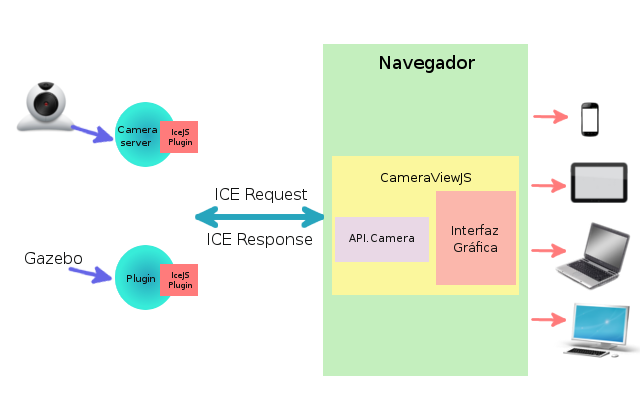
\includegraphics[width=0.8\textwidth]{../traspas/img/esq_cameraviewjs.png}
\caption{Arquitectura de CameraViewJS} \label{fig:cameraviewjs}
\end{figure}

La variable \texttt{config} para crearlo contiene:
\begin{itemize}
 \item \emph{serv:} direcci�n y puerto del servidor (dir:address, port:port).
 \item \emph{camepname:} \textit{endpoint} del servidor, por defecto ``cameraA''.
 \item \emph{camid:} id del canvas que muestra la imagen.
 \item \emph{fpsid:} id del elemento donde se pone el FPS.
\end{itemize}

\subsection{Conector}
El �nico conector que utiliza \texttt{CameraViewJS} es \textbf{API.Camera}:

Al igual que todos los conectores para sensores, su funcionamiento es el siguiente (detallado en la figura \ref{fig:mensajes_camera}): 
En el momento de crear el objeto se establecen las variables de configuraci�n y se crea el \textit{\textit{WebWorker}}. 
Mediante la funci�n \texttt{connect} se establece una promesa que se resuelve una vez est� establecida la conexi�n con el servidor.
Para ello se manda un mensaje al \textit{\textit{WebWorker}} indicando que se conecte y �ste a su vez comienza la conexi�n con el servidor. 
Una vez establecida se env�a al hilo principal un mensaje indicando que est� establecida y �ste resuelve la promesa. 
\lstset{language=JavaScript}
\begin{lstlisting}
    this.connect = function (){
      this.conPromise = new Promise(
        // The resolver function is called with the ability to resolve or
        // reject the promise
        function(resolve, reject) {
            self.w.onmessage = function(mes){
               if (mes.data){
                  self.isRunning = true;
                  resolve();
               }else{
                  self.isRunning = false;
                  reject();
               }
            };
            self.w.postMessage({func:"connect",serv:self.server,epname: self.epname}); 
        });
     
   };
\end{lstlisting}

Todas las funciones que se ejecuten, ya sea pidiendo o enviando datos se quedan paradas esperando a que se resuelva y una vez hecho se ejecutan con normalidad. 
\begin{lstlisting}
    this.getImage = function(){
      this.conPromise.then(
        function() {
            self.w.onmessage = self.onmessage || self.onmessageDefault;
            self.w.postMessage({func:"getImage", imgFormat: self.imgFormat});
        }); 
      
   };
\end{lstlisting}
En el caso de los sensores se puede iniciar un \textit{streaming} que consiste en darle la orden al \textit{WebWorker} y �ste se dedica a hacer peticiones 
al servidor una tras otra y a devolver el resultado al hilo principal hasta que se le indique que pare.
\begin{lstlisting}
    this.startStreaming = function(){
      this.conPromise.then(
        function() {
            self.w.onmessage = self.onmessage || self.onmessageDefault;
            self.w.postMessage({func:"startImageStream", imgFormat: self.imgFormat});
            self.toError=setTimeout(self.conErr, self.timeoutE);
        }); 
   };
   
   this.stopStreaming = function(){
      this.conPromise.then(
        function() {
            self.w.postMessage({func:"stopImageStream"});
            if(self.toError){
               clearTimeout(self.toError);
               toError=undefined;
            }
        }); 
   };
\end{lstlisting}

\begin{figure}[htb]
\centering
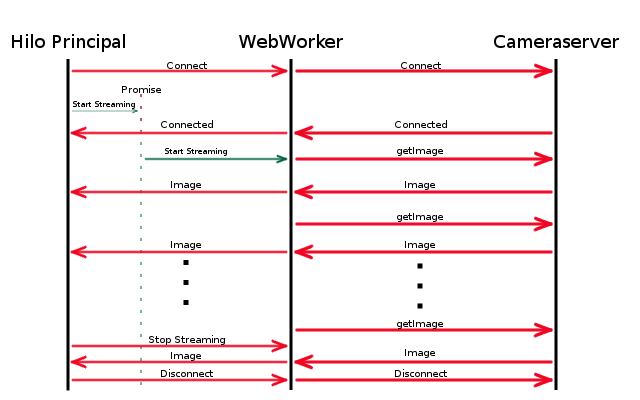
\includegraphics[width=1\textwidth]{./img/mensajes_cameraview.png}
\caption{Mensajes API.Camera.} \label{fig:mensajes_camera}
\end{figure}

Hablando ya en concreto de \texttt{API.Camera}, permite conectar con la interfaz Camera de JdeRobot. El contenido de \texttt{config} es el siguiente:
\begin{itemize}
 \item \emph{server:} direcci�n y puerto del servidor (dir:address, port:port).
 \item \emph{epname:} \textit{endpoint} del servidor, por defecto ``cameraA''.
 \item \emph{imgFormat:} formato de imagen que se va a pedir al servidor, por defecto ``RGB8''.
\end{itemize}

El contenido de la variable \texttt{data} (datos recibidos de la c�mara) es el siguiente:
\begin{itemize}
 \item \emph{width:} Ancho en p�xeles de la imagen recibida.
 \item \emph{height:} Alto en p�xeles de la imagen recibida.
 \item \emph{imgData:} Imagen preparada para ser mostrada en un \texttt{canvas} de HTML5.
 \item \emph{pixelData:} Imagen recibida desde el servidor.
 \item \emph{fps:} fotogramas por segundo recibidos.
\end{itemize}

y su lista de m�todos es:

\begin{itemize}
 \item \emph{createWork:} Crea el \textit{\textit{WebWorker}} (se ejecuta cuando se crea el conector).
 \item \emph{deleteWork:} Elimina el \textit{\textit{WebWorker}}.
 \item \emph{connect:} Inicia la conexi�n con el servidor.
 \item \emph{disconnect:} Desconecta del servidor.
 \item \emph{getImage:} Pide una imagen al servidor.
 \item \emph{startStreaming:} Activa el \textit{streaming} de im�genes (es como ejecutar \texttt{getImage} constantemente).
 \item \emph{stopStreaming:} Detiene el \textit{streaming} de im�genes.
 \item \emph{getDescription:} Pide la descripci�n de la c�mara al servidor y la almacena en la variable \texttt{description}.
\end{itemize}

\subsection{N�cleo}
Cuando se inicia el cliente \textbf{CameraViewJS}, �ste inicia un \textit{streaming} en el \texttt{API.Camera}. Cada vez que se recibe la imagen, 
crea un \texttt{canvas} nuevo donde poner la imagen de la c�mara recibida, despu�s lo introduce como si fuera una foto en el \texttt{canvas} dado en la configuraci�n. 
Esto se hace porque usando un solo \texttt{canvas} si se cambia el tama�o de la p�gina web, por ejemplo, girando la tablet se deforma la imagen recibida de la c�mara. 
Mientras que de esta manera se adapta la imagen al tama�o del \texttt{canvas} externo como si fuera cualquier archivo de imagen. 

%, el \texttt{canvas} externo cambia de tama�o con la web y adapta su contenido a su tama�o, si no se usar un segundo \texttt{canvas}, o no se podr�a adaptar el tama�o 
%de la imagen al dispositivo o se tendr�a que recortar.
\lstset{language=JavaScript}
\begin{lstlisting}
    camera.onmessage = function (event){
         camera.onmessageDefault(event);
         var respwork = camera.data;
         //camera
         var canvas2 = document.createElement('canvas');
         var ctx2=canvas2.getContext("2d");       
         var imgData=ctx2.getImageData(0,0,respwork.width,respwork.height);
         ctx2.canvas.width=respwork.width;
         ctx2.canvas.height=respwork.height;
         var ctx=canvas.getContext("2d");
         imgData.data.set(respwork.imgData);
         ctx2.putImageData(imgData,0,0);
         ctx.drawImage(canvas2, 0, 0,ctx.canvas.width,ctx.canvas.height);
         
         //FPS
         if (respwork.fps){
            fps.html(Math.floor(respwork.fps));
         }
      };
\end{lstlisting}

\subsection{Interfaz gr�fico}

Para la interfaz de los clientes se ha optado por un color oscuro de fondo para reducir el consumo de las pantallas de los dispositivos. Adem�s se usa \textbf{Bootstrap} 
para todos los elementos, organizaci�n y para hacer la web responsiva (se adapta a cualquier dispositivo), como se puede ver en la figura \ref{fig:interfaz_cameraview}.


\begin{figure}[htb]
\centering
\subfigure[]{\label{fig:interfaz_cameraview1}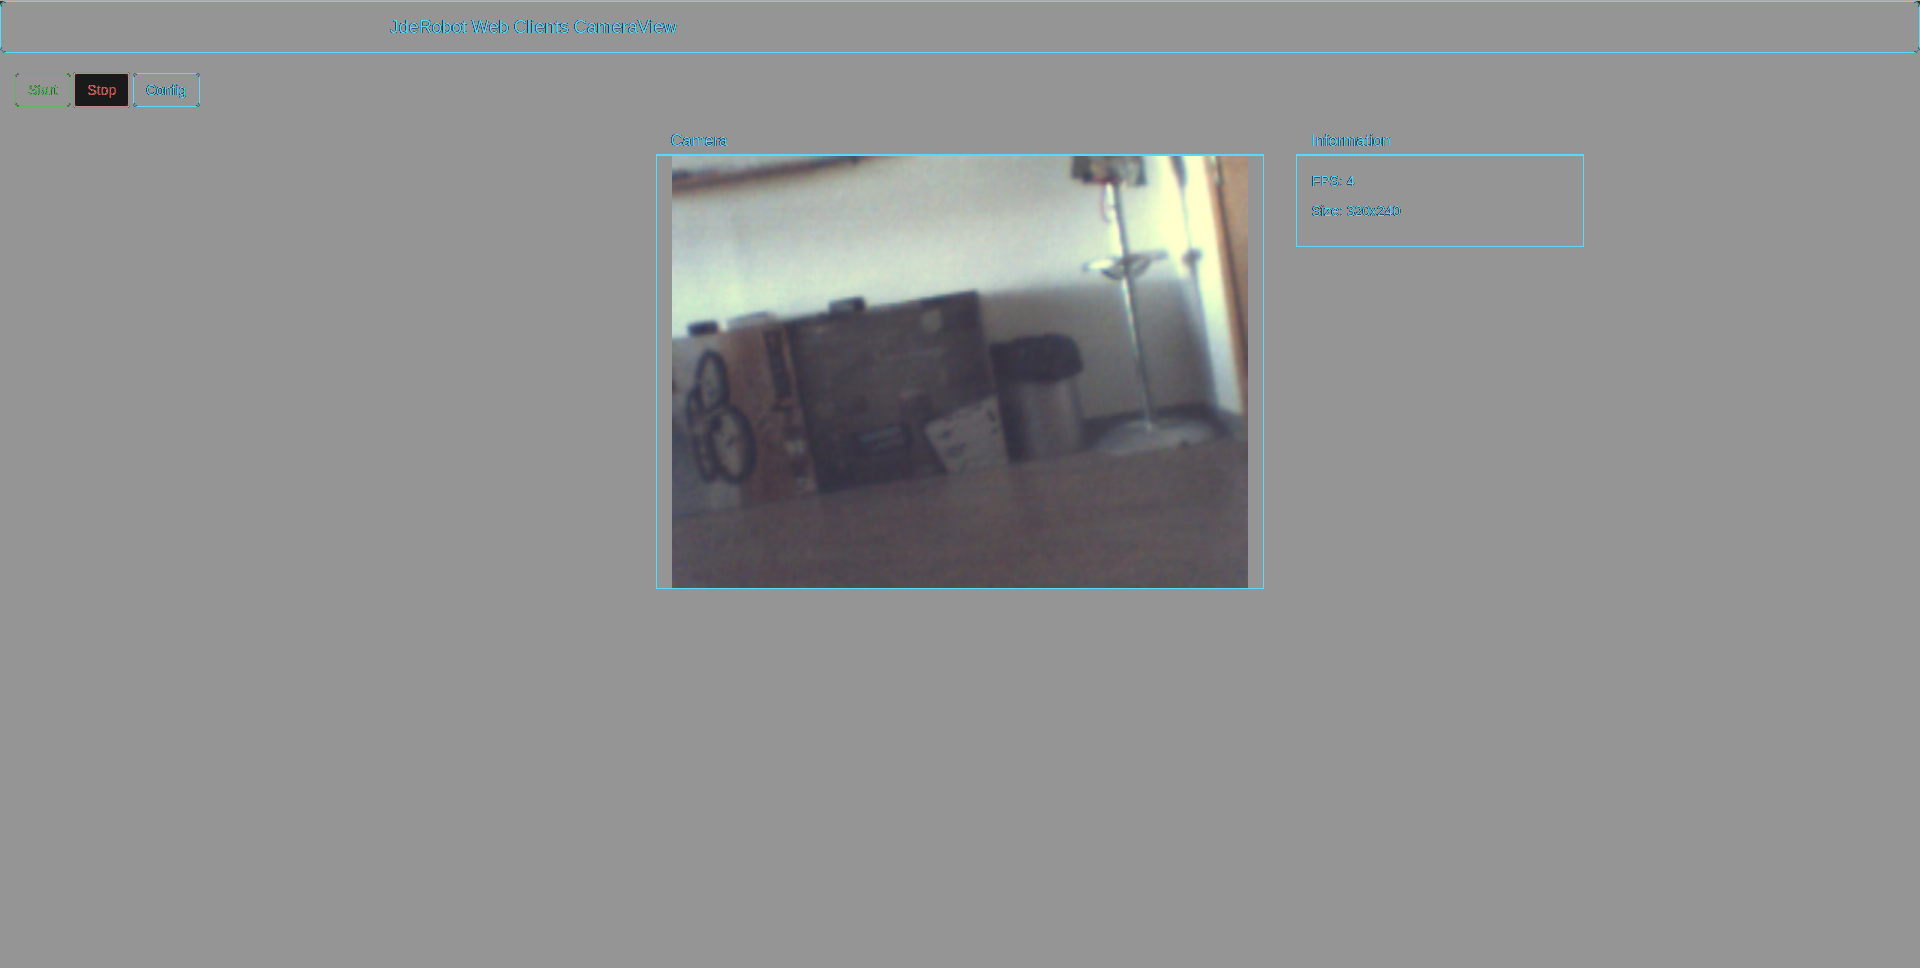
\includegraphics[width=0.6\textwidth]{./img/interfaz_cameraview1.png}}
\hspace{1cm}
\subfigure[]{\label{fig:interfaz_cameraview2}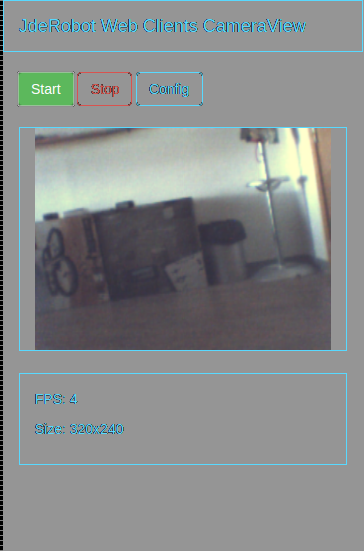
\includegraphics[width=0.3\textwidth]{./img/interfaz_cameraview2.png}}
\caption{Escritorio (a) y M�vil (b)}
\label{fig:interfaz_cameraview}
\end{figure}

La interfaz de cada cliente consta de un fichero HTML y varios CSS y JavaScript.
El \textit{body} de del HTML se divide es 3 partes (figura \ref{fig:jrwc_partes}):

\begin{figure}[htb]
\centering
\subfigure[]{\label{fig:jrwc_partes1}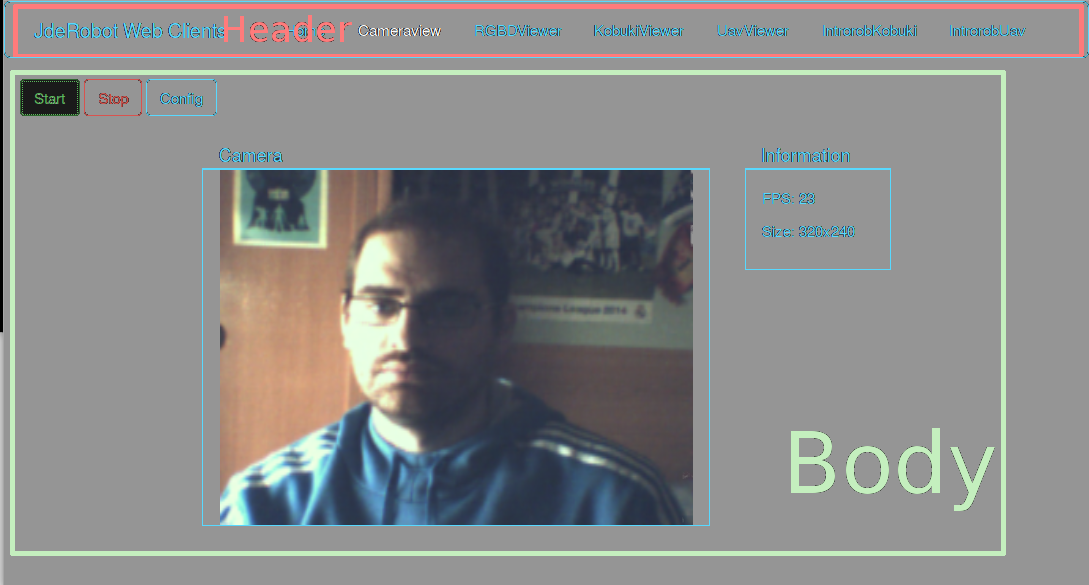
\includegraphics[width=0.45\textwidth]{./img/jrwc_partes.png}}
\hspace{1cm}
\subfigure[]{\label{fig:jrwc_partes2}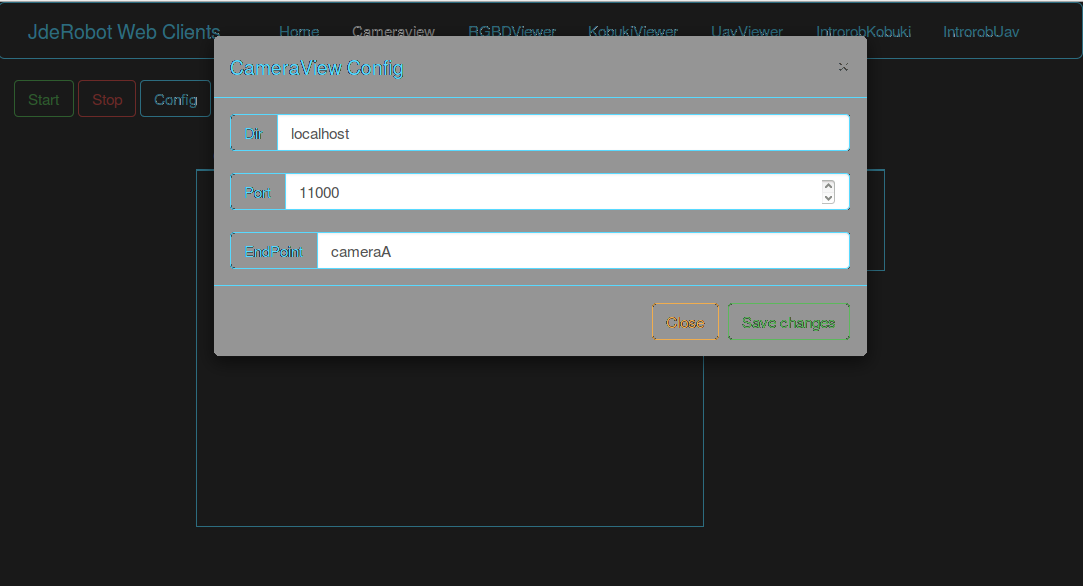
\includegraphics[width=0.45\textwidth]{./img/jrwc_modal.png}}
\caption{Header y Body (a) y Modal (b)}
\label{fig:jrwc_partes}
\end{figure}

\begin{itemize}
 \item \textbf{\textit{Header}}: En todos es igual y contiene la cabecera de la p�gina web.
 \lstset{language=html}
 \begin{lstlisting}
<header id="header">
  <nav class="navbar navbar-inverse" role="banner">
    <div class="container">
      <div class="navbar-header">
        <a class="navbar-brand" href="#"><i class="fa fa-bolt"></i> JdeRobot Web Clients</a></a> </div>
    </div>
    <!--/.container--> 
  </nav>
  <!--/nav--> 
</header>
\end{lstlisting}

\item \textbf{\textit{Body}}: es completamente diferente en cada cliente y contiene los \textit{widgets} propios de cada uno. En el caso de \texttt{CameraViewJS} consta de 3 botones (\texttt{start, stop, config}),
el \texttt{canvas} para mostrar la imagen de la c�mara y un cuadro donde se muestran los FPS y el tama�o de la imagen recibida.

 \lstset{language=html}
 \begin{lstlisting}
<div id="body" class="container">
   <div class="row">
      <div id="buttons" class="col-xs-12 col-sm-12 col-md-12 col-lg-12">
         <p>
            <button id="start" type="button" class="btn btn-md btn-success">Start</button>
            <button id="stop" type="button" class="btn btn-md btn-danger">Stop</button>
            <button id="config" type="button" class="btn btn-info" data-toggle="modal" data-target="#configure">Config</button>
         </p>
      </div>
   </div>
   <div class="row">
      <div class="col-xs-12 col-sm-8 col-md-6 col-lg-4 col-lg-offset-4 col-md-offset-2">
         <div class="border-carbon panel panel-info">
            <div class=" letrero panel-heading hidden-sm hidden-xs">
               <span class="panel-title">Camera</span>
            </div>
            <div class="panel-body padding0 border-blue container-fluid">
               <canvas id="camView" class="col-xs-12 col-sm-12 col-md-12 col-lg-12 cam">Your browser does not support the HTML5 canvas tag.</canvas>
            </div>
         </div>
      </div>
      <div class="col-xs-12 col-sm-2 col-md-2 col-lg-2">
         <div class="border-carbon panel panel-info">
            <div class=" letrero panel-heading hidden-sm hidden-xs">
               <span class="panel-title">Information</span>
            </div>
            <div class="panel-body border-blue container-fluid">
               <p><span class="bold">FPS: </span><span id="fps"></span></p>
               <p><span class="bold">Size: </span><span id="size"></span></p>
            </div>
         </div>
      </div>
   </div>
</div>
\end{lstlisting}

\item \textbf{\textit{Modal}}: Contiene un formulario para guardar la configuraci�n de cada cliente y la �nica diferencia entre los clientes es en el n�mero de elementos del formulario.

 \lstset{language=html}
 \begin{lstlisting}
<div class="modal fade" id="configure" tabindex="-1" role="dialog" aria-labelledby="configLabel">
  <div class="modal-dialog" role="document">
    <div class="modal-content bg-carbon">
      <div class="modal-header bg-orange">
        <button type="button" class="close" data-dismiss="modal" aria-label="Close"><span aria-hidden="true">&times;</span></button>
        <h4 class="modal-title" id="configLabel">CameraView Config</h4>
      </div>
      <div class="modal-body">
         <div class="input-group">
            <span class="input-group-addon" id="basic-addon1">Dir</span>
           <input  id="dir" type="text" class="form-control" placeholder="Direction" value="localhost" aria-describedby="basic-addon1">
         </div>
         <br>
         <div class="input-group">
            <span class="input-group-addon" id="basic-addon1">Port</span>
            <input  id="port" type="number" class="form-control" value="11000" aria-describedby="basic-addon1">
         </div>
         <br>
         <div class="input-group">
            <span class="input-group-addon" id="basic-addon1">EndPoint</span>
            <input id="ep" type="text" class="form-control" value="cameraA" aria-describedby="basic-addon1">
         </div>
      </div>
      <div class="modal-footer">
        <button type="button" class="btn btn-warning" data-dismiss="modal">Close</button>
        <button id="save" type="button" class="btn btn-success" data-dismiss="modal">Save changes</button>
      </div>
    </div>
  </div>
</div>
\end{lstlisting}
\end{itemize}

Debajo de estos tres grandes bloques ya se sit�an los ficheros JavaScript necesarios para cada cliente As� se agiliza la carga de la web.

\clearpage

\section{RgbdViewerJS}
Este cliente se conecta con un servidor de \texttt{Openni1Server} y muestra en dos \texttt{Canvas} de HTML5 la imagen RGB y la de distancia. Los fotogramas por segundo (FPS) de cada imagen se muestran en su respectivo nodo HTML, 
adem�s en un tercer \texttt{canvas} muestra en 3D una escena de la combinaci�n de estas dos im�genes(figura \ref{fig:rgbdviewerjs}). Este �ltimo elemento es la gran diferencia respecto al cliente anterior.

\begin{figure}[htb]
\centering
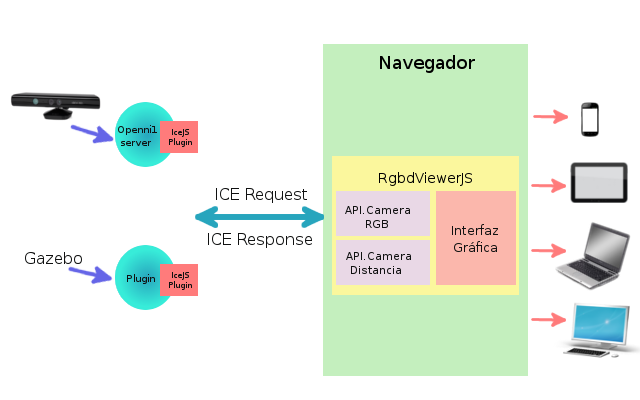
\includegraphics[width=0.8\textwidth]{../traspas/img/esq_rgbdviewerjs.png}
\caption{Arquitectura de RgbdViewerJS} \label{fig:rgbdviewerjs}
\end{figure}

La variable \texttt{config} para crearlo contiene:
\begin{itemize}
 \item \emph{serv:} direcci�n y puerto del servidor (dir:address, port:port).
 \item \emph{camepname:} \textit{endpoint} del servidor de RGB, por defecto ``cameraA''.
 \item \emph{camid:} id del canvas que muestra la imagen RGB.
 \item \emph{fpscamid:} id del elemento donde se pone el FPS RGB.
 \item \emph{depepname:} \textit{endpoint} del servidor de distancia, por defecto ``cameraB''.
 \item \emph{depthid:} id del canvas que muestra la imagen de distancia.
 \item \emph{fpsdepid:} id del elemento donde se pone el FPS de la camara de distancia.
 \item \emph{modelid:} id del canvas que muestra la reconstrucci�n 3D.
\end{itemize}

Este cliente usa dos \textit{conectores} API.Camera, ya explicados en \texttt{CameraViewJS}. El intercambio de mensajes con el servidor es el mismo que en el cliente anterior.

\subsection{N�cleo}

Cuando se inicia el cliente, �ste inicia un \textit{streaming} en los dos \texttt{API.Camera} y se crea el entorno ThreeJS para mostrar la escena. El tratamiento de las im�genes recibidas es el mismo que en 
\texttt{CameraViewJS} pero a�adiendo el procesado necesario para crear la escena 3D (figura \ref{fig:mezcla_imagen}). 


\begin{figure}[htb]
\centering
\subfigure[]{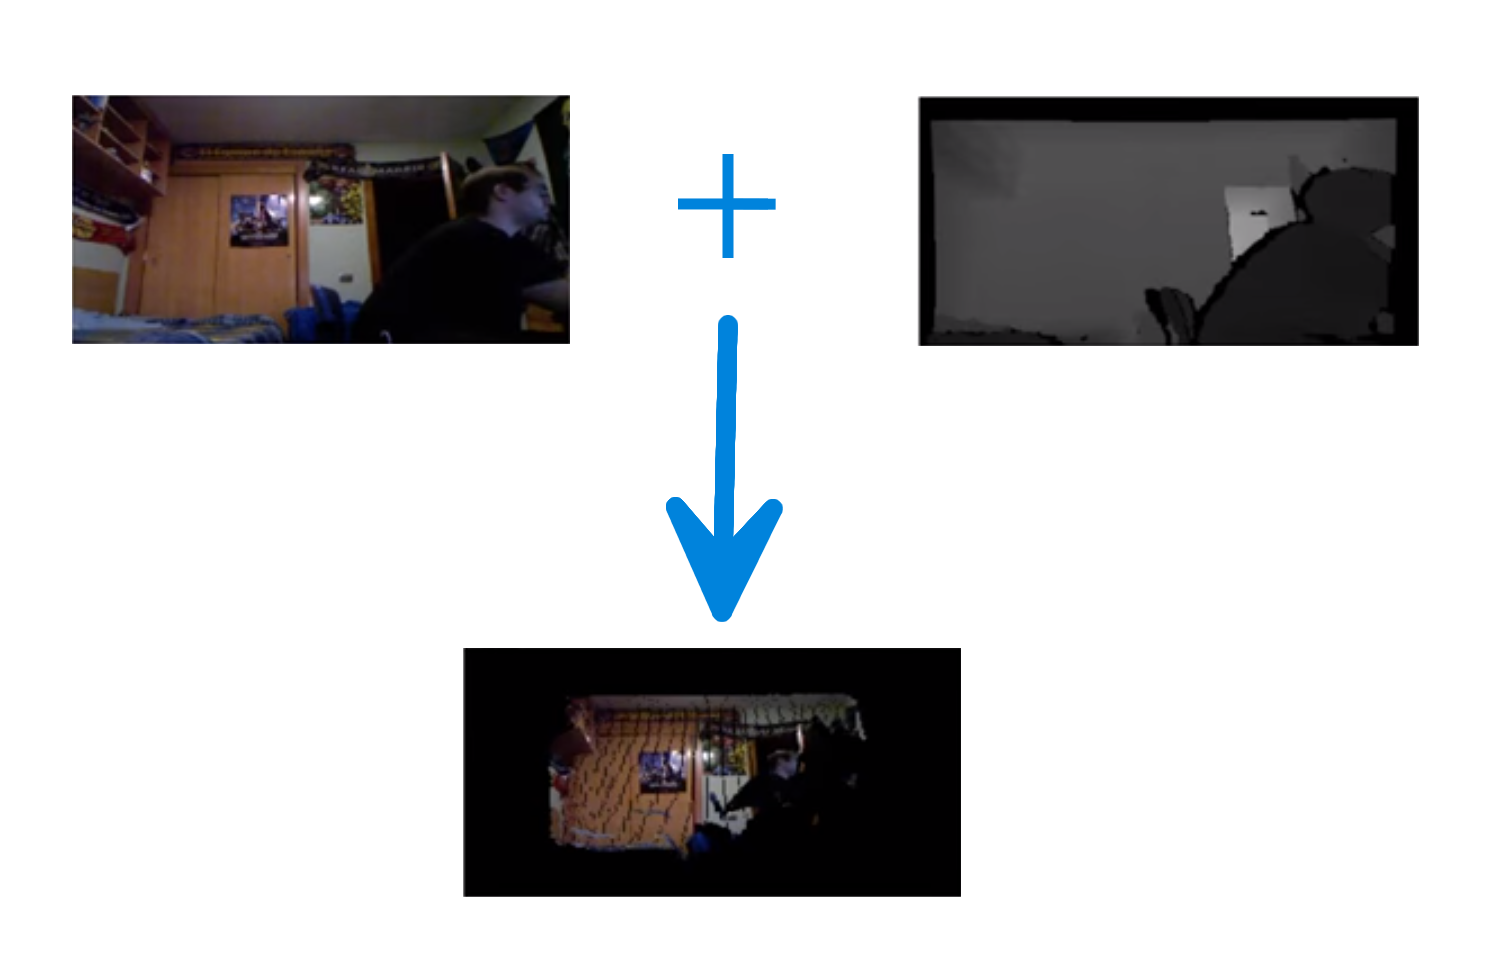
\includegraphics[width=0.8\textwidth]{./img/mezcla_imagenes.png}}
\subfigure[]{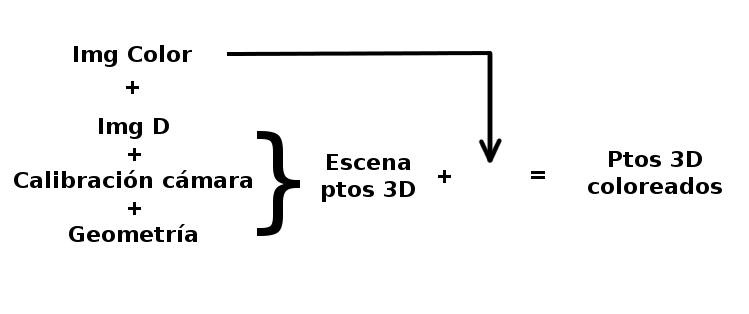
\includegraphics[width=0.8\textwidth]{./img/mezcla_img_texto.png}}
\caption{Creaci�n de la escena 3D} \label{fig:mezcla_imagen}
\end{figure}

Para crearla primero hay que crear un \textit{buffer} de puntos con sus respectivas coordenadas 3D, adem�s de otro \textit{buffer} con el 
color, en formato RGB, que se va a aplicar en cada punto. Para crear el primer \textit{buffer} partimos de la imagen de distancia que s�lo nos da valores del eje Z. Aplicando el modelo \textit{Pin Hole}, 
mostrado en la figura \ref{fig:pinhole}, se ha creado una adaptaci�n de la librer�a \texttt{Progeo} ya existente en JdeRobot para JavaScript y que permite mediante la aplicaci�n de una matriz de traslaci�n y rotaci�n 
pasar de los p�xeles y el valor Z de cada uno a una coordenada (X,Y,Z) real. Dicha matriz se calcula mediante las coordenadas del Kinect y sus �ngulos sobre los ejes con las siguientes f�rmulas:


\begin{figure}[htb]
\centering
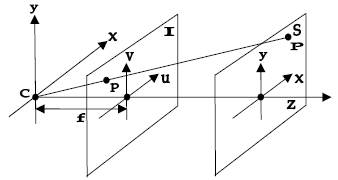
\includegraphics[width=0.5\textwidth]{./img/pinhole.png}
\caption{Modelo de c�mara Pin Hole} \label{fig:pinhole}
\end{figure}

\lstset{language=JavaScript}
\begin{lstlisting}
      rt[0][0] = Math.cos(this.roll) * Math.cos(this.pitch);
      rt[0][1] = (-Math.sin(this.roll) * Math.cos(this.yaw) + Math.cos(this.roll) * Math.sin(this.pitch) * Math.sin(this.yaw);
      rt[0][2] = (Math.sin(this.roll) * Math.sin(this.yaw) + Math.cos(this.roll) * Math.sin(this.pitch) * Math.cos(this.yaw);
      rt[0][3] = this.position.x;
      rt[1][0] = Math.sin(this.roll) * Math.cos(this.pitch);
      rt[1][1] = (Math.cos(this.roll) * Math.cos(this.yaw) + Math.sin(this.roll) * Math.sin(this.pitch) * Math.sin(this.yaw);
      rt[1][2] = (-Math.cos(this.roll) * Math.sin(this.yaw) + Math.sin(this.roll) * Math.sin(this.pitch) * Math.cos(this.yaw);
      rt[1][3] = this.position.y;
      rt[2][0] = Math.sin(this.pitch);
      rt[2][1] = Math.cos(this.pitch) * Math.sin(this.yaw);
      rt[2][2] = Math.cos(this.yaw) * Math.cos(this.pitch);
      rt[2][3] = this.position.z;
      rt[3][0] = 0;
      rt[3][1] = 0;
      rt[3][2] = 0;
      rt[3][3] = 1;
\end{lstlisting}

Una vez hecho esto s�lo hay que aplicar la Matriz a cada punto y ya se tendr�a el \textit{buffer} de puntos en 3D, el \textit{buffer} RGB es el valor RGB del p�xel en dicha imagen.

\lstset{language=JavaScript}
\begin{lstlisting}
      p.x = point.x * rt[0][0] + 
            point.y * rt[0][1] +
            point.z * rt[0][2] +
            point.h * rt[0][3];
   
      p.y = point.x * rt[1][0] + 
            point.y * rt[1][1] +
            point.z * rt[1][2] +
            point.h * rt[1][3];
   
      p.z = - point.x * rt[2][0] + 
            point.y * rt[2][1] +
            point.z * rt[2][2] +
            point.h * rt[2][3];
   
      p.h = point.x * rt[3][0] +
            point.y * rt[3][1] +
            point.z * rt[3][2] +
            point.h * rt[3][3];
\end{lstlisting}

Cuando ya se tienen los dos \textit{buffers} se crea la nube de puntos, se borra la anterior nube y se agrega al modelo 3D la nueva.

\lstset{language=JavaScript}
\begin{lstlisting}
      //prepare the points and each point color
      for (var i=0; i<depth.data.length;i+=depth.width*3*SAMPLE){
         x=-depth.width/2;
         for (var j=0; j<depth.width*3;j+=3*SAMPLE){
            z=(depth.data[i+j+1]<<8) + depth.data[i+j+2]);
            points[a]=x;
            points[a+1]=y;
            points[a+2]=z;

            color.setRGB(rgb.data[i+j]/255,rgb.data[i+j+1]/255,rgb.data[i+j+2]/255);

            colors[ a ]     =color.r;
            colors[ a+ 1 ] =color.g;
            colors[ a+ 2 ] = color.b;
            
            a+=3;
         
            x+=(w/depth.width)*SAMPLE;
         }
         y+=(h/depth.height)*SAMPLE;
      }
      
      var hpoints = conicProjectionCloudHPoint3D(cloudPoint2CloudHPoint3D(points),tphCamera);
      var cloudpoint = cloudHPoint3D2CloudPoint(hpoints);
   
   
      //I do the object using the points, its color and a material that shows the color of each point
      var geometry = new THREE.BufferGeometry();
      geometry.addAttribute( 'position', new THREE.BufferAttribute( new Float32Array(cloudpoint), 3 ) );
      geometry.addAttribute( 'color', new THREE.BufferAttribute( new Float32Array(colors), 3 ) );
   
      var material = new THREE.PointsMaterial( {  vertexColors: THREE.VertexColors} );
      image= new THREE.Points( geometry, material);
  
      if (lastCP){
         scenegl.remove(lastCP);
      }
      scenegl.add(image);
      lastCP=image;
      
      
      depth.update=false;
      rgb.update=false;

   }
\end{lstlisting}

\subsection{Interfaz gr�fico}

C�mo ya se coment� en \texttt{CameraViewJS}, el elemento \texttt{header} y el elemento \texttt{modal} vienen a ser iguales con alguna peque�a modificaci�n, 
por lo que nos centramos ahora en el elemento \texttt{body}.

\begin{figure}[htb]
\centering
\subfigure[]{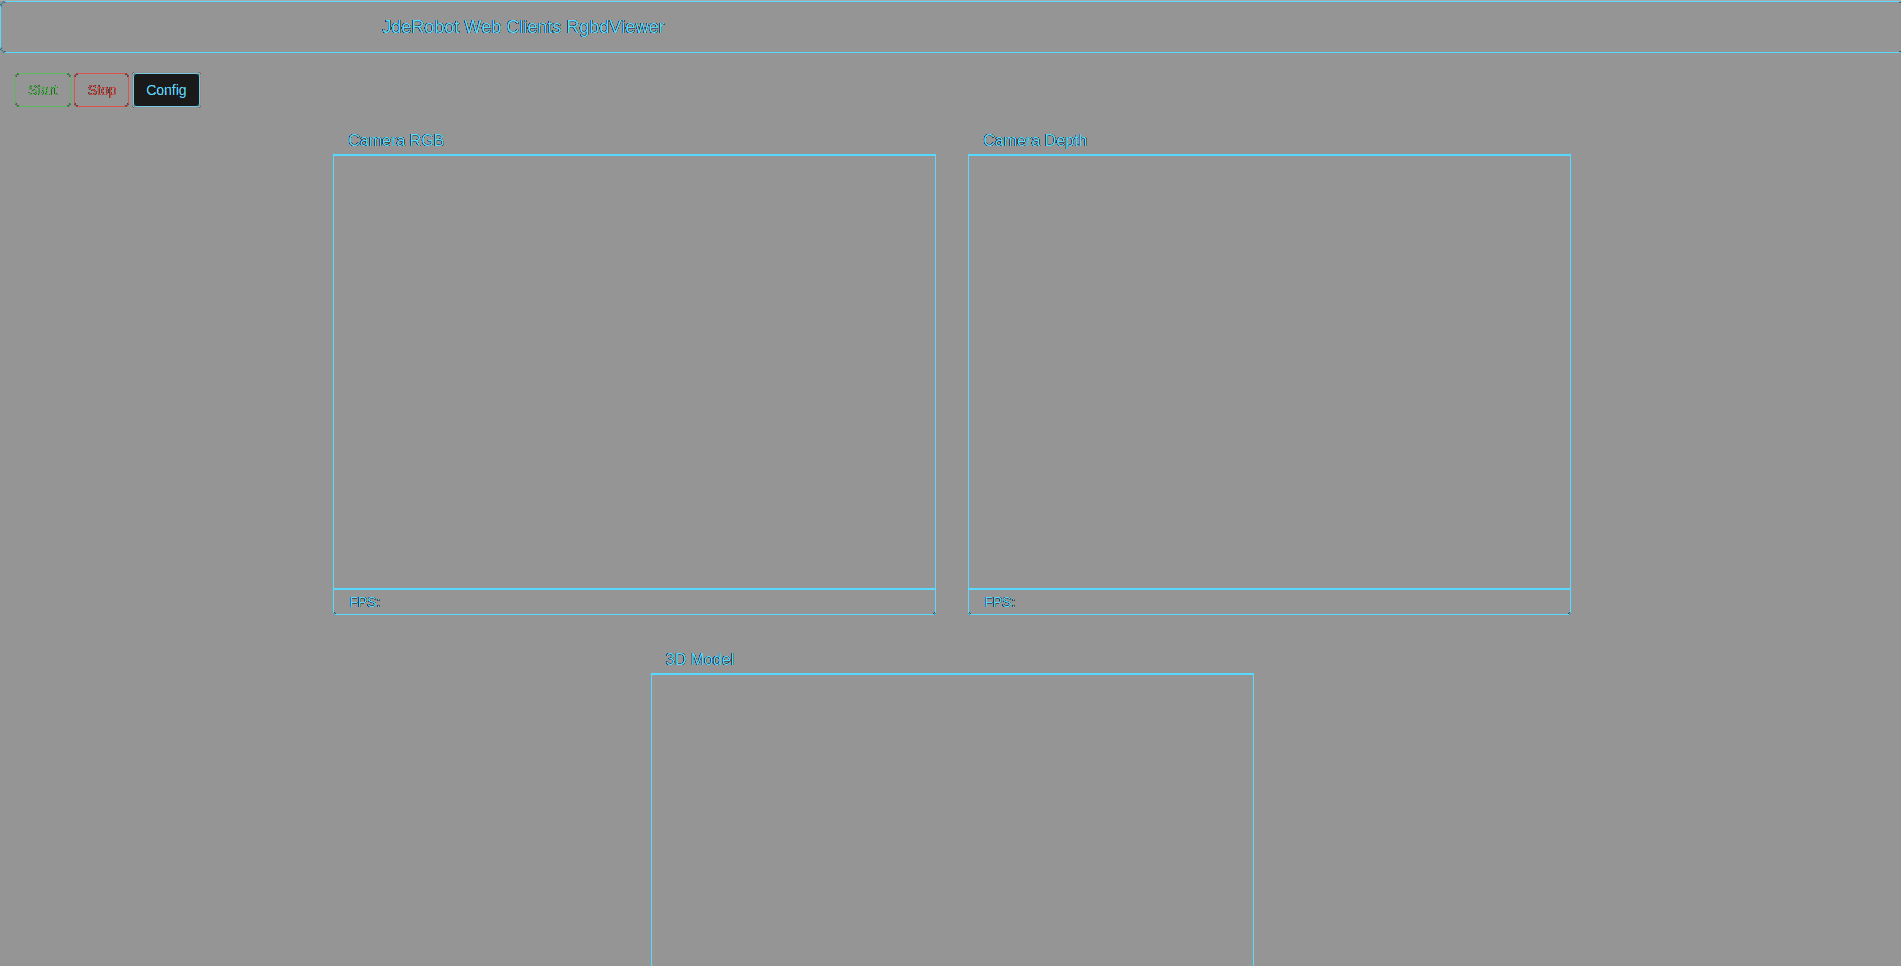
\includegraphics[width=0.45\textwidth]{./img/rgdviewer_init.png}}
\hspace{1cm}
\subfigure[]{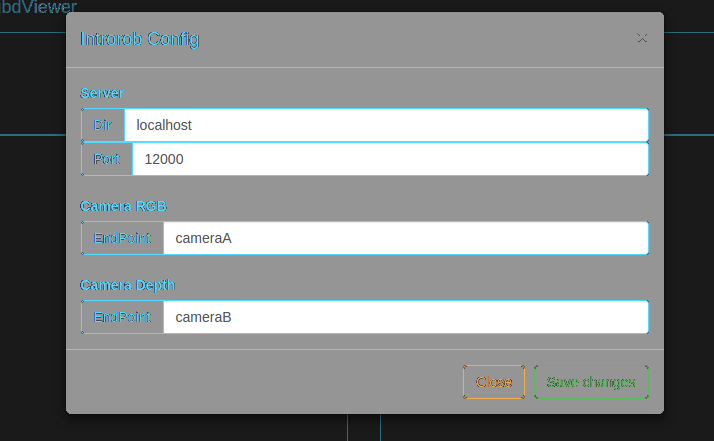
\includegraphics[width=0.45\textwidth]{./img/rgbdviewer_modal.png}}
\caption{Interfaz (a) y Modal (b)}
\label{fig:rgbdviewer_interfaz}
\end{figure}

El \texttt{body} consta de 3 \texttt{canvas} ordenados mediante el sistema \textit{Grid} de Bootstrap, los dos de arriba para las im�genes RGB y de distancia, con un hueco debajo para poner los 
fotogramas por segundo de cada imagen y el tercero para la escena 3D (figura \ref{fig:rgbd_viewer_body}).

\begin{figure}[htb]
\centering
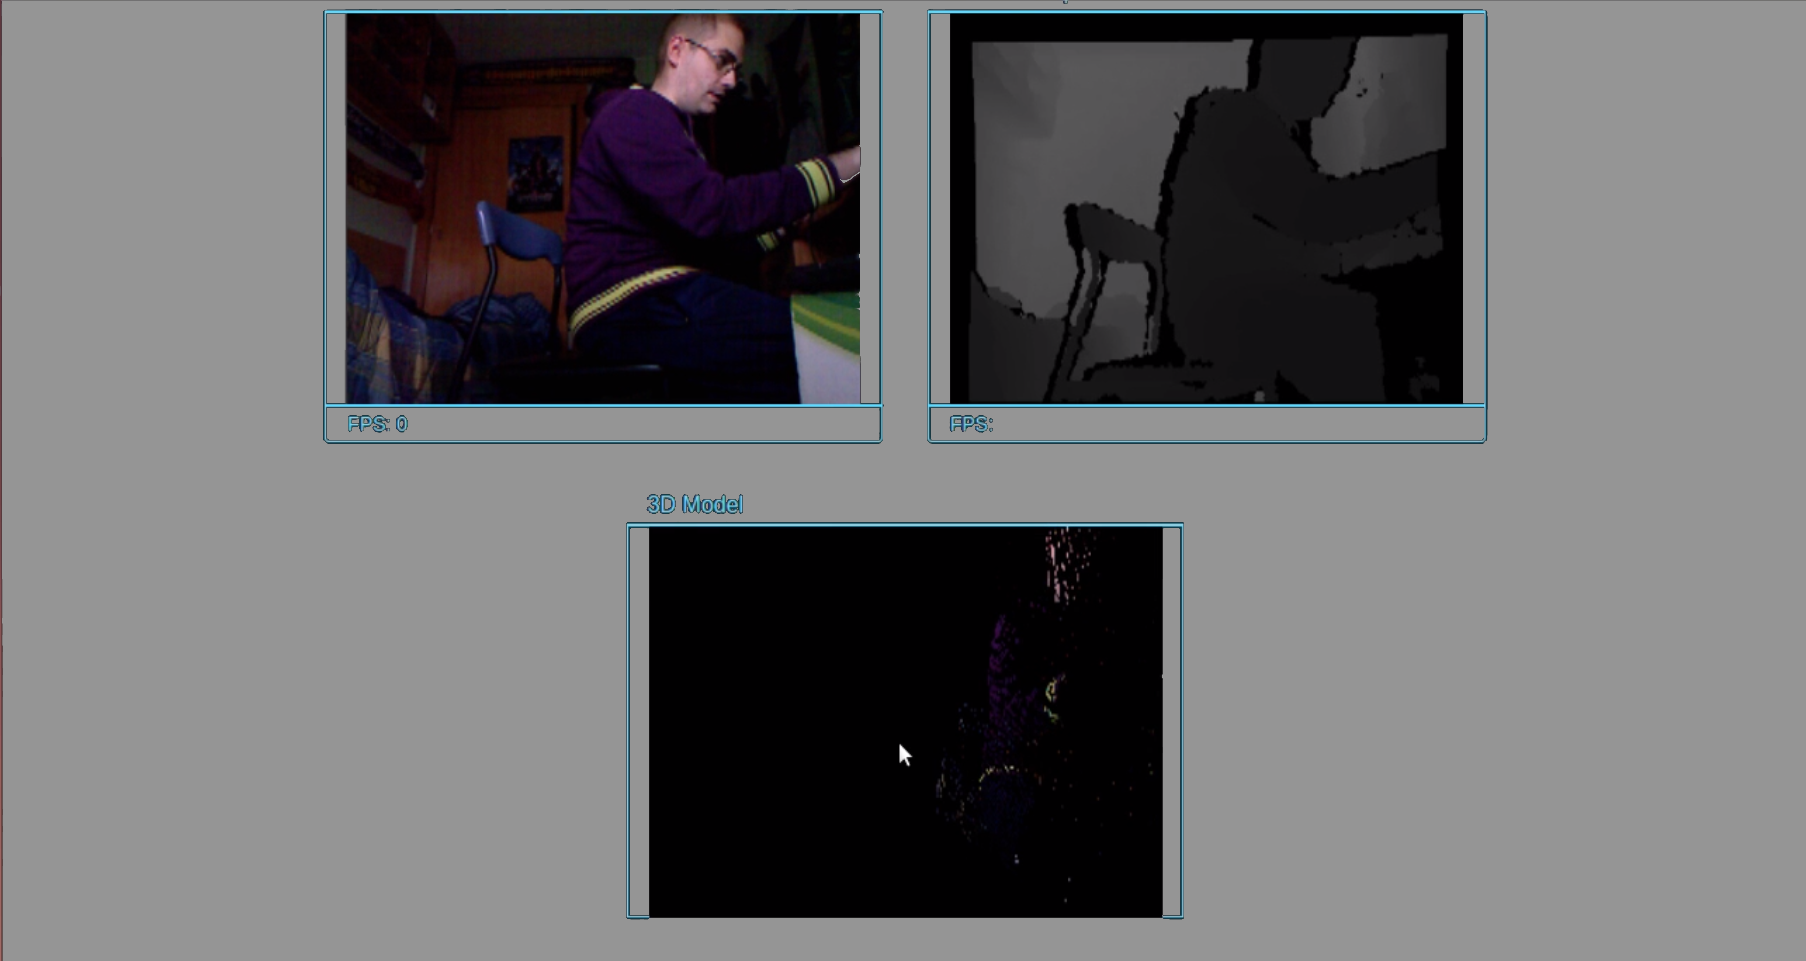
\includegraphics[width=0.5\textwidth]{./img/rgbdviewer12.png}
\caption{Body de RgbdViewerJS} \label{fig:rgbd_viewer_body}
\end{figure}

\lstset{language=html}
\begin{lstlisting}
<div id="body" class="container">
   <div class="row">
      <div id="buttons" class="col-xs-12 col-sm-12 col-md-12 col-lg-12"><p>
        <button id="start" type="button" class="btn btn-md btn-success">Start</button>
        <button id="stop" type="button" class="btn btn-md btn-danger">Stop</button>
        <button id="config" type="button" class="btn btn-info" data-toggle="modal" data-target="#configure">Config</button>
      </p>
      </div>
   </div>
   <div class="row">
      <div class="col-xs-12 col-sm-8 col-md-6 col-lg-4 col-lg-offset-2 col-md-offset-1">
         <div class="border-carbon panel panel-info">
            <div class=" letrero panel-heading hidden-sm hidden-xs">
               <span class="panel-title">Camera RGB</span>
            </div>
            <div class="panel-body padding0 border-blue container-fluid">
               <canvas id="camView" class="col-xs-12 col-sm-12 col-md-12 col-lg-12 cam">Your browser does not support the HTML5 canvas tag.</canvas>
            </div>
            <div class="panel-footer border-blue letrero"><span class="bold">FPS: </span><span id="fps"></span></div>
         </div>
      </div>
      <div class="col-xs-12 col-sm-8 col-md-6 col-lg-4">
         <div class="border-carbon panel panel-info">
            <div class=" letrero panel-heading hidden-sm hidden-xs">
               <span class="panel-title">Camera Depth</span>
            </div>
            <div class="panel-body padding0 border-blue container-fluid">
               <canvas id="camView2" class="col-xs-12 col-sm-12 col-md-12 col-lg-12 cam">Your browser does not support the HTML5 canvas tag.</canvas>
            </div>
            <div class="panel-footer border-blue letrero"><span class="bold">FPS: </span><span id="fps2"></span></div>
         </div>
      </div>
   </div>
      
   <div class="row">
      <div class="col-xs-12 col-sm-8 col-md-6 col-lg-4 col-lg-offset-4 col-md-offset-2">
         <div class="border-carbon panel panel-info">
            <div class=" letrero panel-heading hidden-sm hidden-xs">
               <span class="panel-title">3D Model</span>
            </div>
            <div class="panel-body padding0 border-blue container-fluid">
               <canvas id="model" class="col-xs-12 col-sm-12 col-md-12 col-lg-12 cam">Your browser does not support the HTML5 canvas tag.</canvas>
            </div>
         </div>
      </div>
   </div>
</div>
\end{lstlisting}

Adem�s, en este modelo se puede manejar la c�mara de observaci�n de la escena para poder ver la reconstrucci�n desde distintos puntos de vista (figura \ref{fig:rgbdviewer_modelo3d})

\begin{figure}[!h]
\centering
\subfigure[]{\includegraphics[width=0.45\textwidth]{./img/modelo3d1.png}}
\subfigure[]{\includegraphics[width=0.45\textwidth]{./img/modelo3d2.png}}
\caption{Visualizaci�n con c�maras de observaci�n de frente (a) y a la derecha (b)}
\label{fig:rgbdviewer_modelo3d}
\end{figure}

%\clearpage
\section{KobukiViewerJS}
Este cliente se conecta con un robot con ruedas, modelo Kobuki, para poderlo teleoperar desde la web. Para ello usa dos \texttt{API.Camera}, un \texttt{API.Laser}, un \texttt{API.Pose3D} y un \texttt{API.Motors} (figura \ref{fig:kobukiviewerjs}).

\begin{figure}[htb]
\centering
\includegraphics[width=0.8\textwidth]{../traspas/img/esq_kobukiviewer.png}
\caption{Arquitectura de KobukiViewerJS} \label{fig:kobukiviewerjs}
\end{figure}

La variable \texttt{config} para crearlo contiene:
\begin{itemize}
 \item \emph{camleftserv:} direcci�n y puerto del servidor de la c�mara izquierda (dir:address, port:port).
 \item \emph{camleftepname:} \textit{endpoint} del servidor de la c�mara izquierda.
 \item \emph{camleftid:} id del canvas que muestra la imagen de la c�mara izquierda.
 \item \emph{camrightserv:} direcci�n y puerto del servidor de la c�mara derecha (dir:address, port:port).
 \item \emph{camrightepname:} \textit{endpoint} del servidor de la c�mara derecha.
 \item \emph{camrightid:} id del canvas que muestra la imagen de la c�mara derecha.
 \item \emph{motorserv:} direcci�n y puerto del servidor de los motores (dir:address, port:port).
 \item \emph{motorsepname:} \textit{endpoint} del servidor de los motores.
 \item \emph{controlid:} id del canvas que muestra el control para teleoperar el robot.
 \item \emph{modelid:} id del canvas que muestra una representaci�n en 3D del robot.
 \item \emph{stopbtnid:} id del bot�n que detiene el robot.
 \item \emph{pose3dserv:} direcci�n y puerto del servidor de Pose3D(dir:address, port:port).
 \item \emph{pose3depname:} \textit{endpoint} del servidor de Pose3D.
 \item \emph{laserserv:} direcci�n y puerto del servidor del l�ser(dir:address, port:port).
 \item \emph{laserepname:} \textit{endpoint} del servidor del l�ser.
 \item \emph{laserid:} id del canvas que muestra una representaci�n en 2D del l�ser.
\end{itemize}

\subsection{Conectores}

\texttt{KobukiViewerJS} utiliza 4 conectores: \texttt{API.Camera, API.Laser, API.Pose3D y API.Motors}. 
\texttt{API.Camera} ya est� explicado anteriormente, as� que vamos a seguir por los dem�s.

\textbf{API.Laser}, como todo conector con sensores, b�sicamente funciona igual que API.Camera, pero con las siguientes diferencias:

Permite conectar con la interfaz Laser de JdeRobot. El contenido de \texttt{config} es el siguiente:
\begin{itemize}
 \item \emph{server:} direcci�n y puerto del servidor {(dir:address, port:port)}.
 \item \emph{epname:} \textit{endpoint} del servidor, por defecto ``Laser''.
\end{itemize}

El contenido de la variable \texttt{data} es el siguiente:
\begin{itemize}
 \item \emph{distanceData:} Array de distancias recibidas del servidor.
 \item \emph{numLaser:} N�mero de l�seres recibidos del servidor.
 \item \emph{canv2dData:} Representaci�n de \texttt{distanceData} para ser mostrada en un canvas de HTML5.
 \item \emph{array3dData:} Representaci�n de \texttt{distanceData} para ser mostrada en el modelo 3D.
\end{itemize}

y su lista de m�todos es:

\begin{itemize}
 \item \emph{createWork:} Crea el \textit{\textit{WebWorker}} (se ejecuta cuando se crea el conector).
 \item \emph{deleteWork:} Elimina el \textit{\textit{WebWorker}}.
 \item \emph{connect:} Inicia la conexi�n con el servidor.
 \item \emph{disconnect:} Desconecta del servidor.
 \item \emph{getLaser:} Pide una medida de l�seres al servidor.
 \item \emph{startStreaming:} Activa el \texttt{Streaming} de \texttt{Laser} (es como ejecutar \texttt{getLaser} constantemente).
 \item \emph{stopStreaming:} Detiene el \texttt{Streaming} de \texttt{Laser}.
\end{itemize}

A \textbf{API.Pose3D} le pasa lo mismo que a API.Laser:

Permite conectar con la interfaz Pose3D de JdeRobot. El contenido de \texttt{config} es el siguiente:
\begin{itemize}
 \item \emph{server:} direcci�n y puerto del servidor {(dir:address, port:port)}.
 \item \emph{epname:} \textit{endpoint} del servidor, por defecto ``Pose3D''.
\end{itemize}

El contenido de la variable \texttt{data} es el siguiente:
\begin{itemize}
 \item \emph{x,y,z:} Coordenadas X,Y,Z que representa la posici�n del robot en el espacio.
 \item \emph{q0,q1,q2,q3:} cuaterni�n que representa la orientaci�n del robot.
 \item \emph{yaw,pitch,roll:} Tambi�n representan la orientaci�n pero de manera m�s c�moda de usar, son en radianes.
\end{itemize}

y su lista de m�todos es:

\begin{itemize}
 \item \emph{createWork:} Crea el \textit{\textit{WebWorker}} (se ejecuta cuando se crea el conector).
 \item \emph{deleteWork:} Elimina el \textit{\textit{WebWorker}}.
 \item \emph{connect:} Inicia la conexi�n con el servidor.
 \item \emph{disconnect:} Desconecta del servidor.
 \item \emph{getPose3D:} Pide un Pose3D al servidor.
 \item \emph{startStreaming:} Activa el \texttt{Streaming} de Pose3D (es como ejecutar \texttt{getPose3D} constantemente).
 \item \emph{stopStreaming:} Detiene el \texttt{Streaming} de Pose3D.
\end{itemize}

El caso de \texttt{API.Motors} ya es algo diferente porque ya no conecta con un sensor, sino con un actuador. La parte de la conexi�n con el servidor es igual, 
pero ya el intercambio de mensajes es diferente, porque en este caso se env�an datos en vez de recibirlos (figura \ref{fig:mensajes_motors})

\begin{figure}[htb]
\centering
\includegraphics[width=1\textwidth]{./img/mensajes_motors.png}
\caption{Mensajes API.Motors} \label{fig:mensajes_motors}
\end{figure}

\textbf{API.Motors} permite conectar con la interfaz Motors de JdeRobot. El contenido de \texttt{config} es el siguiente:
\begin{itemize}
 \item \emph{server:} direcci�n y puerto del servidor {(dir:address, port:port)}.
 \item \emph{epname:} \textit{endpoint} del servidor, por defecto ``Motors''.
\end{itemize}

El contenido de la variable \texttt{data} es el siguiente:
\begin{itemize}
 \item \emph{v,w,l:} velocidades recibidas del servidor.
\end{itemize}

y su lista de m�todos es:

\begin{itemize}
 \item \emph{createWork:} Crea el \textit{\textit{WebWorker}} (se ejecuta cuando se crea el conector).
 \item \emph{deleteWork:} Elimina el \textit{\textit{WebWorker}}.
 \item \emph{connect:} Inicia la conexi�n con el servidor.
 \item \emph{disconnect:} Desconecta del servidor.
 \item \emph{getV:} Pide la velocidad V al servidor.
 \item \emph{getW:} Pide la velocidad W al servidor.
 \item \emph{getL:} Pide la velocidad L al servidor.
 \item \emph{setV:} Env�a la velocidad V al servidor.
 \item \emph{setW:} Env�a la velocidad W al servidor.
 \item \emph{setL:} Env�a la velocidad L al servidor.
 \item \emph{setAll:} Env�a todas las velocidades al servidor.
\end{itemize}


\subsection{N�cleo}
Cuando se inicia el cliente \texttt{KobukiViewerJS}, �ste inicia un \textit{streaming} de los sensores y se crean el control y la representaci�n 3D. El tratamiento de las im�genes recibidas es el mismo que en \texttt{CameraViewJS}. 
Para el control se ha creado un peque�o componente que permite dibujar el Joystick en un \texttt{canvas} (figura \ref{fig:control}) y que permite dar comportamiento a las interacciones del rat�n sobre �ste, permitiendo enviar velocidades los motores.

\lstset{language=JavaScript}
\begin{lstlisting}
   control = new GUI.Control ({id:self.controlid});
      
      control.lastW=0;
      control.lastV=0;
      
      //comportamiento cuando se mueve el Joystick
      control.onPointerM = function (event){
         control.onPointerMDefault(event);
         var distSend = 2;
         var pos = control.position;
         
         if (calcDist(pos.x,control.lastW)>=distSend){
            motors.setW(pos.x/3);
            control.lastW = pos.x;
         }
         
         if (calcDist(pos.z,control.lastV)>=distSend){
            motors.setV(pos.z);
            control.lastV = pos.z;
         } 
      };
      
      control.initControl();
\end{lstlisting}

\begin{figure}[htb]
\centering
\subfigure[]{\label{fig:control}\includegraphics[width=0.40\textwidth]{./img/control1.png}}
\hspace{1cm}
\subfigure[]{\label{fig:kobuki3d}\includegraphics[width=0.40\textwidth]{./img/kobuki3d2.png}}
\caption{Control (a) y Modelo 3D (b)}
\label{fig:control_modelo}
\end{figure}

El bot�n \texttt{stopBot} coloca el Joystick en el centro y env�a velocidades 0 a los motores. Para el modelo 3D (figura \ref{fig:kobuki3d}) se ha creado otro peque�o componente que permite cargar desde modelos \texttt{Collada} 
tanto los robots Pioneer y Kobuki como un Drone. Se ha hecho porque los modelos de los robots ven�an por partes y as� se facilita su uso, adem�s de porque la carga de cada parte es as�ncrona 
y se necesitaba sincronizarlo todo para poder ejecutar una funci�n al final de la carga del modelo.
En esta escena de pinta el robot en la posici�n que indican los sensores.

\lstset{language=JavaScript}
\begin{lstlisting}
  this.loadPioneer = function (scale,onLoad){
      this.minYPos = 0.11;
      this.robot = new THREE.Group();
      var loaded = 2;
      this.manager.onLoad = onLoad;
      var chassisLoader = new THREE.ColladaLoader(self.manager);
      chassisLoader.options.convertUpAxis = true;
      chassisLoader.load(
	        'js/libs/robotloaders/pioneer/chassis.dae',
	        function ( collada ) {
       
		  var obj = collada.scene;
               
		  obj.scale.x =obj.scale.y = obj.scale.z = scale;
		  obj.position.y=(self.minYPos+0.05)*scale;
		  obj.updateMatrix();
       
		  self.robot.add(obj);
		  loaded--;
		  if (loaded==0){
		      onLoad();
		  }
	        });
      
      var wheelLoader = new THREE.ColladaLoader(self.manager);
      wheelLoader.options.convertUpAxis = true;
      wheelLoader.load(
	        'js/libs/robotloaders/pioneer/wheel.dae',
	        function ( collada ) {
       
		    var obj = collada.scene;
		    var obj2 = obj.clone();

		    obj.scale.x =obj.scale.y = obj.scale.z = scale;
		    obj.position.z=-0.17*scale;
		    obj.position.x=0.1*scale;
		    obj.position.y=self.minYPos*scale;
		    obj.updateMatrix();
		    
		    obj2.scale.x =obj2.scale.y = obj2.scale.z = scale;
		    obj2.position.z=0.17*scale;
		    obj2.position.x=0.1*scale;
		    obj2.position.y=self.minYPos*scale;
		    obj2.rotation.y=Math.PI;
		    obj2.updateMatrix();
	    
		    self.robot.add(obj);
		    self.robot.add(obj2);
		    loaded--;
		    if (loaded==0){
			onLoad();
		    }
	        });
\end{lstlisting}

Una vez creado todo el modelo se inician los dos sensores que van a interactuar con �ste, como son el Pose3D, que cada vez que se reciben datos cambia la posici�n y la orientaci�n del robot en el modelo, y el l�ser 
que adem�s de representar en un \texttt{canvas} sus datos en 2D, se a�aden al modelo en 3D (figura \ref{fig:laser}). 

\lstset{language=JavaScript}
\begin{lstlisting}
  loader.loadKobuki(1,function () {
               model.robot=loader.robot;
               model.scene.add( model.robot );
         
               pose3d = new API.Pose3D({server:self.pose3dserv,epname:self.pose3depname});
               pose3d.onmessage= function (event){
                  pose3d.onmessageDefault(event);
                  model.robot.position.set(pose3d.data.x/1000,pose3d.data.z/1000,-pose3d.data.y/1000);
                  model.robot.rotation.y=(pose3d.data.yaw);
                  model.robot.updateMatrix();
                  model.renderer.render(model.scene,model.camera);
               };
         
               pose3d.timeoutE=timeout;
         
               pose3d.connect();
               pose3d.startStreaming();
         
               laser= new API.Laser({server:self.laserserv,epname:self.laserepname,canv2dWidth:lasercanv.width,scale3d:0.001,convertUpAxis:true});
               laser.onmessage= function (event){
                  laser.onmessageDefault(event);
                  //2D
                  var dist = laser.data.canv2dData;
                  var ctx = lasercanv.getContext("2d");
                  ctx.beginPath();
                  ctx.clearRect(0,0,lasercanv.width,lasercanv.height);
                  ctx.fillRect(0,0,lasercanv.width,lasercanv.height);
                  ctx.strokeStyle="white";
                  ctx.moveTo(dist[0], dist[1]);
                  for (var i = 2;i<dist.length; i = i+2 ){
                     ctx.lineTo(dist[i], dist[i+1]);
                  }   
                  ctx.moveTo(lasercanv.width/2, lasercanv.height);
                  ctx.lineTo(lasercanv.width/2, lasercanv.height-10);
                  ctx.stroke();
                  
                  //3D
                  var geometry = new THREE.BufferGeometry();
                  geometry.addAttribute( 'position', new THREE.BufferAttribute( new Float32Array(laser.data.array3dData), 3 ) );
                  var material = new THREE.MeshBasicMaterial( { color: 0x00ff00 } );
                  material.transparent = true;
                  material.opacity=0.5;
                  material.side = THREE.DoubleSide;
		  var las = new THREE.Mesh( geometry, material );
                  if (model.laser){
                     model.robot.remove(model.laser);
                  };
                  model.robot.add(las);
                  model.laser = las;

               };
               laser.connect();
               laser.startStreaming();
               
               modelAnimation();
	        });
\end{lstlisting}

\begin{figure}[htb]
\centering
\subfigure[]{\includegraphics[width=0.45\textwidth]{./img/laser2d.png}}
\hspace{1cm}
\subfigure[]{\includegraphics[width=0.45\textwidth]{./img/laser3d.png}}
\caption{L�ser en 2D (a) y 3D (b)}
\label{fig:laser}
\end{figure}


\subsection{Interfaz gr�fico}

los elementos \texttt{header} y \texttt{modal} son iguales a los de \texttt{CameraViewJS} con alguna peque�a modificaci�n, 
por lo que nos vamos a centrar en el \texttt{body}.

\begin{figure}[htb]
\centering
\subfigure[]{\includegraphics[width=0.55\textwidth]{./img/kobukiviewer_init.png}}
\hspace{1cm}
\subfigure[]{\includegraphics[width=0.25\textwidth]{./img/kobukiviewer_modal.png}}
\caption{Interfaz (a) y Modal (b)}
\label{fig:kobukiviewer_interfaz}
\end{figure}

El \texttt{body} consta de 5 \texttt{canvas} y un bot�n ordenados mediante el sistema \textit{Grid} de Bootstrap. Los dos primeros de arriba para las im�genes de las dos c�maras, 
el tercero para el l�ser en 2D, el cuarto para el modelo 3D  y el quinto para el control (figura \ref{fig:kobukiviewer_body}).

\begin{figure}[htb]
\centering
\includegraphics[width=0.9\textwidth]{./img/kobukiviewer_body.png}
\caption{Body de KobukiViewerJS} \label{fig:kobukiviewer_body}
\end{figure}

\lstset{language=html}
\begin{lstlisting}
<div id="body" class="container">
   <div class="row">
      <div id="buttons" class="col-xs-12 col-sm-12 col-md-12 col-lg-12">
        <p>
           <button id="start" type="button" class="btn btn-md btn-success">Start</button>
           <button id="stop" type="button" class="btn btn-md btn-danger">Stop</button>
           <button id="config" type="button" class="btn btn-info" data-toggle="modal" data-target="#configure">Config</button>
        </p>
      </div>
   </div>
   <div class="row">
      <div class="col-xs-12 col-sm-8 col-md-6 col-lg-4">
         <div class="border-carbon panel panel-info">
            <div class=" letrero panel-heading hidden-sm hidden-xs">
               <span class="panel-title">Camera Left</span>
            </div>
            <div class="panel-body padding0 border-blue container-fluid">
               <canvas id="camView" class="col-xs-12 col-sm-12 col-md-12 col-lg-12 cam">Your browser does not support the HTML5 canvas tag.</canvas>
            </div>
         </div>
      </div>
      <div class="col-xs-12 col-sm-8 col-md-6 col-lg-4">
         <div class="border-carbon panel panel-info">
            <div class=" letrero panel-heading hidden-sm hidden-xs">
               <span class="panel-title">Camera Right</span>
            </div>
            <div class="panel-body padding0 border-blue container-fluid">
               <canvas id="camView2" class="col-xs-12 col-sm-12 col-md-12 col-lg-12 cam">Your browser does not support the HTML5 canvas tag.</canvas>
            </div>
         </div>
      </div>
      <div class="col-xs-12 col-sm-8 col-md-6 col-lg-4">
         <div class="border-carbon panel panel-info">
            <div class=" letrero panel-heading hidden-sm hidden-xs">
               <span class="panel-title">Laser</span>
            </div>
            <div class="panel-body padding0 border-blue container-fluid">
               <canvas id="laser" class="col-xs-12 col-sm-12 col-md-12 col-lg-12">Your browser does not support the HTML5 canvas tag.</canvas>
            </div>
         </div>
      </div>
   </div>
   <div class="row">
      <div class="col-xs-12 col-sm-8 col-md-6 col-lg-4">
         <div class="border-carbon panel panel-info">
            <div class=" letrero panel-heading hidden-sm hidden-xs">
               <span class="panel-title">3D Model</span>
            </div>
            <div class="panel-body padding0 border-blue container-fluid">
               <canvas id="model" class="col-xs-12 col-sm-12 col-md-12 col-lg-12">Your browser does not support the HTML5 canvas tag.</canvas>
            </div>
         </div>
      </div>
      <div class="col-xs-12 col-sm-8 col-md-6 col-lg-4">
         <div class="border-carbon panel panel-info">
            <div class=" letrero panel-heading hidden-sm hidden-xs">
               <span class="panel-title">Control</span>
            </div>
            <div class="panel-body padding0 border-blue container-fluid">
               <canvas id="control" class="col-xs-12 col-sm-12 col-md-12 col-lg-12">Your browser does not support the HTML5 canvas tag.</canvas>
            </div>
         </div>
      </div>
      <div class="col-xs-6 col-sm-4 col-md-2 col-lg-2">
         <button id="stopR" type="button" class="btn btn-info" >Stop Bot</button>
      </div>
   </div>
</div>
\end{lstlisting}

Por �ltimo, cabe destacar que la escena 3D del robot usa exactamente el mismo control de c�mara que el usado en \texttt{RgbdViewerJS} (figura \ref{fig:kobukiviewer_camera}), 
de modo que la c�mara de observaci�n de la escena 3D se puede mover y girar a voluntad.
\begin{figure}[htb]
\centering
\subfigure[]{\includegraphics[width=0.45\textwidth]{./img/kobuki3d.png}}
\hspace{1cm}
\subfigure[]{\includegraphics[width=0.45\textwidth]{./img/kobuki3d2.png}}
\caption{Visualizaci�n 3D del robot con zoom (b) y sin �l (a).}
\label{fig:kobukiviewer_camera}
\end{figure}

%\clearpage
\section{UavViewerJS}
Este cliente se conecta con un drone para poderlo teleoperar desde la web. Para ello usa un \texttt{API.Camera}, un \texttt{API.Pose3D}, un \texttt{API.CmdVel} y un \texttt{API.Extra} (figura \ref{fig:uavviewerjs}).

\begin{figure}[htb]
\centering
\includegraphics[width=0.8\textwidth]{../traspas/img/esq_uavviewer.png}
\caption{Arquitectura de UavViewerJS} \label{fig:uavviewerjs}
\end{figure}

La variable \texttt{config} para crearlo contiene:
\begin{itemize}
 \item \emph{cam1serv:} direcci�n y puerto del servidor de la c�mara(dir:address, port:port).
 \item \emph{cam1epname:} \textit{endpoint} del servidor de la c�mara.
 \item \emph{cam1id:} id del canvas que muestra la imagen de la c�mara.
 \item \emph{cmdvelserv:} direcci�n y puerto del servidor de la velocidad (dir:address, port:port).
 \item \emph{cmdvelepname:} \textit{endpoint} del servidor de la velocidad.
 \item \emph{control1id, control2id:} id de los canvas de los controles.
 \item \emph{modelid:} id del canvas que muestra una representaci�n en 3D del drone.
 \item \emph{pose3dserv:} direcci�n y puerto del servidor de Pose3D (dir:address, port:port).
 \item \emph{pose3depname:} \textit{endpoint} del servidor de Pose3D.
 \item \emph{takeoffbtnid:} id del bot�n que despega el drone.
 \item \emph{stopbtnid:} id del bot�n que detiene el drone.
 \item \emph{landbtnid:} id del bot�n que aterriza el drone.
 \item \emph{resetbtnid:} id del bot�n que resetea el drone.
 \item \emph{extraserv:} \textit{endpoint} del servidor de ArDroneExtra, funciones propias del drone.
 \item \emph{extraepname:} direcci�n y puerto del servidor del interfaz Extra(dir:address, port:port).
 \item \emph{attitudeid, headingid, altimeterid, turn\_coordinatorid:} ids de los indicadores de vuelo.
\end{itemize}

\subsection{Conectores}
Tanto \texttt{API.Camera} como \texttt{API.Pose3D} ya est�n descritos en los clientes anteriores, por lo que vamos a describir los nuevos conectores.

\textbf{API.ArDroneExtra} permite conectar con la interfaz ArDroneExtra de JdeRobot. El contenido de \texttt{config} es el siguiente:
\begin{itemize}
 \item \emph{server:} direcci�n y puerto del servidor {(dir:address, port:port)}.
 \item \emph{epname:} \textit{endpoint} del servidor, por defecto ``Extra''.
\end{itemize}

y su lista de m�todos es:

\begin{itemize}
 \item \emph{createWork:} Crea el \textit{WebWorker} (se ejecuta cuando se crea el conector).
 \item \emph{deleteWork:} Elimina el \textit{WebWorker}.
 \item \emph{connect:} Inicia la conexi�n con el servidor.
 \item \emph{disconnect:} Desconecta del servidor.
 \item \emph{toggleCam:} Cambia de c�mara del drone.
 \item \emph{land:} Aterriza el drone.
 \item \emph{takeoff:} Despega el drone.
\end{itemize}

\texttt{API.CmdVel}, como todo conector con actuadores, b�sicamente funciona igual que \texttt{API.Motors}, pero con las siguientes diferencias:
permite conectar con la interfaz CmdVel de JdeRobot. El contenido de \texttt{config} es el siguiente:
\begin{itemize}
 \item \emph{server:} direcci�n y puerto del servidor {(dir:address, port:port)}.
 \item \emph{epname:} \textit{endpoint} del servidor, por defecto ``CmdVel''.
\end{itemize}

y su lista de m�todos es:

\begin{itemize}
 \item \emph{createWork:} Crea el \textit{WebWorker} (se ejecuta cuando se crea el conector).
 \item \emph{deleteWork:} Elimina el \textit{WebWorker}.
 \item \emph{connect:} Inicia la conexi�n con el servidor.
 \item \emph{disconnect:} Desconecta del servidor.
 \item \emph{setCmdVel:} Env�a las velocidades al servidor (\texttt{linearX, linearY, linearZ, angularX, angularY, angularZ};).
\end{itemize}

\subsection{N�cleo}

Cuando se inicia el cliente, �ste inicia un \textit{streaming} de los sensores y se crean dos controles y la representaci�n 3D. El tratamiento de las im�genes recibidas es el mismo que en \texttt{CameraViewJS}. 
Los controles son los mismos que los creados para \texttt{KobukiViewerJS}, pero cada uno controla dos velocidades.

\lstset{language=JavaScript}
\begin{lstlisting}
      control1 = new GUI.Control ({id:self.control1id});
      control2 = new GUI.Control ({id:self.control2id});
 
      control1.onPointerM = function (event){
         control1.onPointerMDefault(event);
         var distSend = 1;
         var pos = control1.position;
         var send = false;
         if (calcDist(pos.x,cmdSend.linearY)>=distSend){
            cmdSend.linearY = pos.x/2;
            send = true;
         }   
         if (calcDist(pos.z,cmdSend.linearX)>=distSend){
            cmdSend.linearX = pos.z/2;
            send = true;
         }
         if (send){
            cmdvel.setCmdVel(cmdSend);
         }       
      };
      
     control2.onPointerM = function (event){
         control2.onPointerMDefault(event);
         var distSend = 2;
         var pos = control2.position;
         var send = false;
         if (calcDist(pos.x/10,cmdSend.angularZ)>=distSend){
            cmdSend.angularZ = pos.x/10;
            send = true;
         } 
         if (calcDist(pos.z/2,cmdSend.linearZ)>=distSend){
            cmdSend.linearZ = pos.z/2;
            send = true;
         }
         if (send){
            cmdvel.setCmdVel(cmdSend);
         } 
      };
      
      control1.initControl();
      control2.initControl();
\end{lstlisting}

El bot�n \texttt{stop drone}, coloca los Joystick en el centro y env�a velocidades 0 a los motores, el resto de botones ejecutan las funciones hom�nimas de API.ArDroneExtra (figura \ref{fig:dronebuttons}).

\begin{figure}[htb]
\centering
\includegraphics[width=0.7\textwidth]{./img/uavviewerjs_extra.png}
\caption{Botones de funciones del drone} \label{fig:dronebuttons}
\end{figure}

Para el modelo 3D se ha usado el mismo componente que en \texttt{KobukiViewerJS}, una vez creado el modelo se inicia el Pose3D y 
cada vez que se recibe informaci�n de �ste var�a la posici�n del modelo (figura \ref{fig:drone_uav}) y de los indicadores de vuelo\footnote{\url{https://github.com/sebmatton/jQuery-Flight-Indicators}} (figura \ref{fig:indicadores}).

\begin{figure}[htb]
\centering
\subfigure[]{\label{fig:drone_uav}\includegraphics[width=0.35\textwidth]{./img/uavviewer3d.png}}
\hspace{1cm}
\subfigure[]{\label{fig:indicadores}\includegraphics[width=0.55\textwidth]{./img/indicadores.png}}
\caption{Modelo 3D (a) e indicadores de vuelo (b)}
\label{fig:uavviewer_drone}
\end{figure}

\lstset{language=JavaScript}
\begin{lstlisting}
  loader.loadQuadrotor(0.05,function () {
               model.robot=loader.robot;
               model.scene.add( model.robot );
         
               pose3d = new API.Pose3D({server:self.pose3dserv,epname:self.pose3depname});
               pose3d.onmessage= function (event){
                  pose3d.onmessageDefault(event);
                  model.robot.position.set(pose3d.data.x,pose3d.data.z,-pose3d.data.y);
                  model.robot.rotation.set(pose3d.data.pitch,pose3d.data.yaw,pose3d.data.roll);
                  model.robot.updateMatrix();
                  model.renderer.render(model.scene,model.camera);
                  // Attitude update
                  attitude.setRoll(-pose3d.data.roll * toDegrees);
                  attitude.setPitch(-pose3d.data.pitch * toDegrees);

                   // Altimeter update
                   altimeter.setAltitude(pose3d.data.z*100);

                   // TC update
                   turn_coordinator.setTurn(-pose3d.data.roll * toDegrees);

                   // Heading update
                   heading.setHeading(pose3d.data.yaw * toDegrees);
               };
         
               pose3d.timeoutE=timeout;
         
               pose3d.connect();
               pose3d.startStreaming();
               
               modelAnimation();
	        });
\end{lstlisting}

\subsection{Interfaz gr�fico}

C�mo ya se coment� en los anteriores clientes, los elementos \texttt{header} y \texttt{modal} son casi iguales con alguna peque�a modificaci�n, 
por lo que nos vamos a centrar ahora en el \texttt{body}.

\begin{figure}[htb]
\centering
\subfigure[]{\includegraphics[width=0.55\textwidth]{./img/uavviewer_init.png}}
\hspace{1cm}
\subfigure[]{\includegraphics[width=0.25\textwidth]{./img/uavviewer_modal.png}}
\caption{Interfaz (a) y Modal (b)}
\label{fig:uavviewer_interfaz}
\end{figure}

El \texttt{body} consta de 3 filas, la primera contiene el \texttt{canvas} de la c�mara y los indicadores de vuelo, la segunda los \texttt{canvas} del modelo 3D y los controles
y la tercera contiene los botones (figura \ref{fig:uavviewer_body}).

\begin{figure}[htb]
\centering
\includegraphics[width=0.9\textwidth]{./img/uavviewer_body.png}
\caption{Body de UavViewerJS} \label{fig:uavviewer_body}
\end{figure}

\lstset{language=html}
\begin{lstlisting}
<div id="body" class="container">
   <div class="row">
      <div id="buttons" class="col-xs-12 col-sm-12 col-md-12 col-lg-12"><p>
        <button id="start" type="button" class="btn btn-md btn-success">Start</button>
        <button id="stop" type="button" class="btn btn-md btn-danger">Stop</button>
        <button id="config" type="button" class="btn btn-info" data-toggle="modal" data-target="#configure">Config</button>
      </p>
      </div>
   </div>
   <div class="row">
      <div class="col-xs-12 col-sm-8 col-md-6 col-lg-4">
         <div class="border-carbon panel panel-info">
            <div class=" letrero panel-heading hidden-sm hidden-xs">
               <span class="panel-title">Camera</span>
            </div>
            <div class="panel-body padding0 border-blue container-fluid">
               <canvas id="camView" class="col-xs-12 col-sm-12 col-md-12 col-lg-12 cam">Your browser does not support the HTML5 canvas tag.</canvas>
            </div>
         </div>
      </div>
      <div class="col-xs-12 col-sm-12 col-md-6 col-lg-8">
         <div class="border-carbon panel panel-info">
            <div class=" letrero panel-heading hidden-sm hidden-xs">
               <span class="panel-title">Flight Indicators</span>
            </div>
            <div class="panel-body padding0 border-blue container-fluid">
               <span id="attitude"></span>
               <span id="altimeter"></span>
               <span id="turn_coordinator"></span>
               <span id="heading"></span>
            </div>
         </div>
      </div>
   </div>
      
   <div class="row">
      <div class="col-xs-12 col-sm-8 col-md-6 col-lg-4">
         <div class="border-carbon panel panel-info">
            <div class=" letrero panel-heading hidden-sm hidden-xs">
               <span class="panel-title">3D Model</span>
            </div>
            <div class="panel-body padding0 border-blue container-fluid">
               <canvas id="model" class="col-xs-12 col-sm-12 col-md-12 col-lg-12">Your browser does not support the HTML5 canvas tag.</canvas>
            </div>
         </div>
      </div>
      <div class="col-xs-12 col-sm-8 col-md-6 col-lg-4">
         <div class="border-carbon panel panel-info">
            <div class=" letrero panel-heading hidden-sm hidden-xs">
               <span class="panel-title">Control X + Y</span>
            </div>
            <div class="panel-body padding0 border-blue container-fluid">
               <canvas id="control1" class="col-xs-12 col-sm-12 col-md-12 col-lg-12">Your browser does not support the HTML5 canvas tag.</canvas>
            </div>
         </div>
      </div>
      <div class="col-xs-12 col-sm-8 col-md-6 col-lg-4">
         <div class="border-carbon panel panel-info">
            <div class=" letrero panel-heading hidden-sm hidden-xs">
               <span class="panel-title">Control Z + angle of rotation</span>
            </div>
            <div class="panel-body padding0 border-blue container-fluid">
               <canvas id="control2" class="col-xs-12 col-sm-12 col-md-12 col-lg-12">Your browser does not support the HTML5 canvas tag.</canvas>
            </div>
         </div>
      </div>
   </div>
   <div class="row">
      <div id="buttons2" class="btn-toolbar col-xs-12 col-sm-12 col-md-12 col-lg-12" role="toolbar" aria-label="buttons2">
         <div class="btn-group" role="group" aria-label="bextra">
            <button id="takeoff" type="button" class="btn btn-info">Takeoff</button>
            <button id="land" type="button" class="btn btn-info">Land</button>
            <button id="toggle" type="button" class="btn btn-info" >Toggle Camera</button>
         </div>
         <div class="btn-group" role="group" aria-label="stp">
            <button id="stopb" type="button" class="btn btn-info" >Stop drone</button>
         </div>
      </div>
   </div>
</div>
\end{lstlisting}

\clearpage
\section{IntrorobKobukiJS}
Este cliente es exactamente el mismo que \texttt{KobukiViewerJS} pero a�adiendo la infraestructura para el comportamiento aut�nomo (figura \ref{fig:introrobkobukijs}), 
por lo que la variable \textbf{config} que recibe el constructor es igual. Se le han a�adido dos m�todos nuevos aparte de los comunes a todos los clientes:
\begin{itemize}
 \item \textit{startMyAlgorithm}: inicia el comportamiento aut�nomo.
 \item \textit{stopMyAlgorithm}: detiene el comportamiento aut�nomo.
\end{itemize}

\begin{figure}[htb]
\centering
\includegraphics[width=0.8\textwidth]{../traspas/img/esq_introrobkobuki.png}
\caption{Arquitectura de IntrorobKobukiJS} \label{fig:introrobkobukijs}
\end{figure}

Utiliza los mismos \textit{conectores} que \texttt{KobukiViewerJS}.

\subsection{N�cleo}
La �nica diferencia con \texttt{KobukiViewerJS} es la opci�n de agregar comportamiento aut�nomo. Cuando se inicia el comportamiento aut�nomo se crea un \textit{WebWorker} donde se ha 
programado dicho comportamiento. 
EL hilo principal cada 100ms le env�a los datos recibidos por los sensores al \textit{WebWorker}, y �ste a su vez, despu�s de ejecutar el comportamiento aut�nomo, 
devuelve una orden de velocidad para los motores (en caso de ser necesario incluso puede detener e iniciar el env�o de datos del hilo principal):

\lstset{language=JavaScript}
\begin{lstlisting}
  this.startMyAlgorithm = function (){
      //document.getElementById(self.controlid).SetActive(false);
      control.removeListeners();
      document.getElementById(self.stopbtnid).disabled = true;
      var f = function(){
         if (laser.data && cameraright.data && pose3d.data && cameraleft.data ){
             var msg ={pose3d:pose3d.data,
                  laser:{distanceData:laser.data.distanceData, numLasers:laser.data.numLaser},
                  camr:{pixelData:cameraright.data.pixelData,height:cameraright.data.height, width:cameraright.data.width},
                  caml:{pixelData:cameraleft.data.pixelData,height:cameraleft.data.height, width:cameraleft.data.width}};
         worker.postMessage(msg);
             }
      };
      worker = new Worker(workerFile);
      worker.onmessage = function (m){
         if (lastV!=m.data.v || lastW!=m.data.w){
            lastV = m.data.v;
            lastW = m.data.w;
            motors.setV(lastV);
            motors.setW(lastW);
         }
         var d = m.data.interval;
         switch (d){
         case 1:
               interval = setInterval(f,100);
               break;
         case 2:
               clearInterval(interval);
               break;
         default:
         
         }
      };
      interval = setInterval(f,100);
\end{lstlisting}

Para detener el comportamiento, se deja de enviar datos al \textit{\textit{WebWorker}} (se detiene el \textit{interval}) y se elimina dicho \textit{worker}. El contenido de fichero \textbf{myalgorithm\_worker.js}, 
que contiene el \textit{script} que va a interpretar el \textit{\textit{WebWorker}} es el siguiente:

\lstset{language=JavaScript}
\begin{lstlisting}
/* Data Recived
 * - laser:
 *       + distanceData : Array of distances
 *       + numLaser: numer of lasers
 * - pose3d:
 *       + x,y,z: coords
 *       + q1,q2,q3,q4 : quaternion
 *       + yaw, pitch, roll: orientation
 * - caml, camr:
 *       + data: Array of Image data
 *       + width, height: width y height of the image, in pixels
 *
 *********************************
 * Data Response
 * - v,w: velocities 
 * - interval: if the action takes more than time reception sensor (100ms). Possible values:
 *   + 0 : do nothing
 *   + 1 : start interval in main thread
 *   + 2 : stop interval in main thread
 */

onmessage = function(e) {
    
   var laser  = e.data.laser;
   var pose3d = e.data.pose3d;
   var caml = e.data.caml;
   var camr = e.data.camr;
   
   var v = 0;
   var w = 0;
          
   
   postMessage({v:v,w:w,interval:0});
}
\end{lstlisting}
Como se puede ver, tiene un primer comentario explicando los datos recibidos y los que se pueden enviar, 
adem�s de la funci�n donde se tiene que programar en JavaScript el comportamiento aut�nomo, con un ejemplo de respuesta.

\subsection{Interfaz gr�fico}

La �nica variaci�n a la interfaz de \texttt{KobukiViewerJS} es que se le ha agregado un bot�n m�s a la botonera para iniciar y detener el comportamiento aut�nomo
(figura \ref{fig:introrobkobuki_interfaz}), que se traduce en eliminar o crear el \textit{WebWorker} subyacente que incluye la l�gica del comportamiento aut�nomo y el \textit{interval} de env�o de datos.
\begin{figure}[htb]
\centering
\includegraphics[width=0.7\textwidth]{./img/introrobkobuki_interfaz.png}
\caption{Interfaz de IntrorobKobukiJS} \label{fig:introrobkobuki_interfaz}
\end{figure}.



\section{IntrorobUavJS}
Es el equivalente a \texttt{IntrorobKobukiJS} pero para drones, por lo que la base es \texttt{UavViewerJS} (figura \ref{fig:introrobuavjs}).
\begin{figure}[htb]
\centering
\includegraphics[width=0.7\textwidth]{../traspas/img/esq_introrobuav.png}
\caption{Arquitectura de IntrorobUavJS} \label{fig:introrobuavjs}
\end{figure}

Utiliza los mismos \textit{conectores} que \texttt{UavViewerJS}.

\subsection{N�cleo}

Es este caso, el mensaje de respuesta del \textit{\textit{WebWorker}} 
es m�s complejo porque se pueden enviar m�s �rdenes que al robot kobuki, por lo tanto el fichero \textbf{myalgorithm\_worker.js} quedar�a as�:

\lstset{language=JavaScript}
\begin{lstlisting}
/* Data Recived
 * - pose3d:
 *       + x,y,z: coords
 *       + q1,q2,q3,q4 : quaternion
 *       + yaw, pitch, roll: orientation
 * - cam1:
 *      + data: Array of Image data
 *      + width, height: width y height of the image, in pixels
 *
 *********************************
 * Data Response
 * - com: command to send to drone. Possible values:
 *   + sendVel : send Velocities 
 *   + takeoff : takeoff drone
 *   + land : land drone
 *   + toggleCam : change camera
 * - linearX,linearY,linearZ,angularZ: velocities 
 * - interval: if the action takes more than time reception sensor (100ms). Possible values:
 *   + 0 : do nothing
 *   + 1 : start interval in main thread
 *   + 2 : stop interval in main thread
 */


onmessage = function(e) {
    
   var pose3d = e.data.pose3d;
   var cam1 = e.data.cam1;
   
   var linearX = 0;
   var linearY = 0;
   var linearZ = 0;
   var angularZ = 0;
   
   postMessage({com:"semdVel",linearX:linearX,linearY:linearY,linearZ:linearZ,angularZ:angularZ,interval:0});
}
\end{lstlisting}

\subsection{Interfaz gr�fico}

La �nica variaci�n a la interfaz de \texttt{UavViewerJS} es que se le ha agregado un bot�n mas a la botonera para iniciar y detener el comportamiento aut�nomo 
(figura \ref{fig:introrobuav_interfaz})
\begin{figure}[htb]
\centering
\includegraphics[width=0.7\textwidth]{./img/introrobuav_interfaz.png}
\caption{Interfaz de IntrorobUavJS} \label{fig:introrobuav_interfaz}
\end{figure}.

\section{JdeRobotWebClients} \label{sec:JdeRobotwebclients}

Adem�s de los seis clientes web descritos
se ha creado un \texttt{index.html} con una peque�a explicaci�n de la p�gina web, como se puede ver en la figura \ref{fig:jrwc_index}, que integra en sendas pesta�as cada uno de ellos.


\begin{figure}[htb]
\centering
\subfigure[]{\label{fig:jrwc_index1}\includegraphics[width=0.6\textwidth]{./img/jrwc_index_desktop.png}}
\hspace{1cm}
\subfigure[]{\label{fig:jrwc_index2}\includegraphics[width=0.3\textwidth]{./img/jrwc_index_phone.png}}
\caption{Escritorio (a) y M�vil (b)}
\label{fig:jrwc_index}
\end{figure}


Cada cliente sigue en un fichero HTML distinto, para permitir separarlos de la web m�s f�cilmente. La �nica modificaci�n que se les ha hecho es a�adir un men� de navegaci�n en el \texttt{header}
para facilitar el cambio entre clientes.
 \lstset{language=html}
 \begin{lstlisting}
<header id="header">
  <nav class="navbar navbar-inverse" role="banner">
    <div class="container">
      <div class="navbar-header">
        <button type="button" class="navbar-toggle" data-toggle="collapse" data-target=".navbar-collapse"> <span class="sr-only">Toggle navigation</span> <span class="icon-bar"></span> <span class="icon-bar"></span> <span class="icon-bar"></span> </button>
        <a class="navbar-brand" href="index.html"><i class="fa fa-bolt"></i> JdeRobot Web Clients</a></a>
     </div>
      <div class="collapse navbar-collapse navbar-right">
        <ul class="nav navbar-nav">
          <li ><a href="index.html">Home</a></li>
          <li class="active"><a href="cameraview.html">Cameraview</a></li>
          <li><a href="rgbdviewer.html">RGBDViewer</a></li>
          <li><a href="kobukiviewer.html">KobukiViewer</a></li>
          <li><a href="uavviewer.html">UavViewer</a></li>
           <li><a href="introrobkobuki.html">IntrorobKobuki</a></li>
           <li><a href="introrobuav.html">IntrorobUav</a></li>
        </ul>
      </div>
    </div>
    <!--/.container--> 
  </nav>
  <!--/nav--> 
</header>
\end{lstlisting}






\chapter{Experimentos}  
\label{ch:Experimentos}

En este cap�tulo se presentan las pruebas realizadas al sistema y el \texttt{hardware} necesario
para la reproducci�n de las mismas. Estos experimentos se dividen en siete pruebas, una por cada cliente 
con el objetivo de comprobar su correcto funcionamiento y una s�ptima de rendimiento temporal de recepci�n de v�deo de las c�maras.

\section{Experimentos con CameraViewJS}
Este experimento consiste en una ejecuci�n t�pica del cliente \texttt{CameraViewJS} desarrollado. Para ello se ejecuta \texttt{cameraserver} 
en un PC y el cliente tanto en otro PC como en un m�vil estando todos en la misma red local.

En la figura \ref{fig:equipos_camview} se puede observar la funci�n que cumplen cada uno de los componentes de las pruebas.
Como servidor de im�genes ICE se utiliz� un ordenador de la universidad
con un procesador Intel(R) Core(TM)2 Quad 2.66GHz con 4GbiB de memoria RAM. En este
PC se instal� la distribuci�n Ubuntu de JdeRobot 5.3.1 y se le conect� la webcam logitech. 
Esta m�quina se usa tanto como servidor \texttt{cameraserver} como servidor HTTP donde albergar los clientes.

Como cliente 1 se utiliz� un port�til Acer Ferrari One 
con un procesador AMD Athlon(tm) Dual Core L310 y 4 GbiB de memoria RAM. En �l se instalaron 
los navegadores Firefox, Chrome y Opera para realizar la pruebas.

Como cliente 2 se utiliz� un \textit{SmartPhone} Elephone P6000 con un procesador MTK6732 de 64Bits a 1.5GHz 
y 2GbiB de memoria RAM. En �l se instalaron los navegadores Firefox, Chrome y Opera para realizar la pruebas.

\begin{figure}[htb]
\centering
\includegraphics[width=0.8\textwidth]{./img/equipos.png}
\caption{Equipos usados en este experimento y su funci�n.} \label{fig:equipos_camview}
\end{figure}


Como se puede ver en las figuras \ref{fig:interfaz_cameraview_exp}, funciona igual tanto en m�vil como en PC. 
La tasa de refresco de las im�genes 
var�a si cliente y servidor se ejecutan en el mismo PC (8 FPS) o en diferente (4 FPS). El tama�o de imagen id�neo es 320x240 p�xeles 
porque m�s peque�as se perder�a mucha calidad y mayores producen un desplome de los fotogramas por segundo hasta quedarse en 2-3 FPS en la misma m�quina.
Adem�s hay que comentar que en algunas de las pruebas se han llegado a conseguir 25 FPS en el mismo PC sin ninguna raz�n aparente porque no se realiz� ning�n cambio, 
lo �nico que se hizo fue parar tanto cliente y servidor y volverlos a arrancar.

\begin{figure}[htb]
\centering
\subfigure[]{\includegraphics[width=0.6\textwidth]{./img/interfaz_cameraview1.png}}
\hspace{1cm}
\subfigure[]{\includegraphics[width=0.3\textwidth]{./img/interfaz_cameraview2.png}}
\caption{Cliente 1 (a) y Cliente 2 (b)}
\label{fig:interfaz_cameraview_exp}
\end{figure}

\section{Experimentos con RgbdViewerJS}
Este experimento consiste en una ejecuci�n t�pica del cliente \texttt{RgbdViewerJS} desarrollado. Para ello se ejecuta \texttt{Openni1Server} 
en un PC teniendo conectado un Kinect y el cliente en otro PC estando todos en la misma red local.

En la figura \ref{fig:equipos_rgbd} se puede observar la funci�n que cumplen cada uno de los componentes de las pruebas.
Como servidor de im�genes RGBD ICE se utiliz� un ordenador de la universidad
con un procesador Intel(R) Core(TM)2 Quad 2.66GHz con 4GbiB de memoria RAM. En este
PC se instal� la distribuci�n Ubuntu de JdeRobot 5.3.1 y se le conect� el Kinect. 
Esta m�quina se usa tanto como servidor \texttt{Openni1Server} como servidor HTTP donde albergar los clientes.

Como cliente se utiliz� un port�til Acer Ferrari One 
con un procesador AMD Athlon(tm) Dual Core L310 y 4 GbiB de memoria RAM. En �l se instalaron 
los navegadores Firefox, Chrome y Opera para realizar el experimento.

\begin{figure}[htb]
\centering
\includegraphics[width=0.8\textwidth]{./img/equipos_rgbdviewerjs.png}
\caption{Equipos usados en estas pruebas y su funci�n.} \label{fig:equipos_rgbd}
\end{figure}

Como se puede ver en la 
figura \ref{fig:interfaz_rgbdviewer_exp}, funciona correctamente. En este caso los experimentos han estado algo limitados debido 
a que para trabajar con el Kinect se necesita mucha capacidad de procesamiento, por lo que rara vez se pasaba de 1 FPS en la recepci�n de las im�genes. Hay que destacar 
que se comprobaron los valores mediante el \texttt{RgbdViewer} escrito en C++ y este no pasaba de 2 FPS as� que asumimos que el \textit{hardware} limitaba dicho experimento.

\begin{figure}[htb]
\centering
\includegraphics[width=0.8\textwidth]{./img/rgbdviewer12.png}
\caption{Ejecuci�n de cliente}
\label{fig:interfaz_rgbdviewer_exp}
\end{figure}

\section{Experimentos con KobukiViewerJS}
Este experimento consiste en una ejecuci�n t�pica del cliente \texttt{KobukiViewerJS} desarrollado tanto en real como simulado. las pruebas consistieron 
en teleoperar un robot Kobuki tanto real como simulado estando cliente y servidor en la misma red local. 

En la figura \ref{fig:equipos_kobukiviewer} se puede observar la funci�n que cumplen cada uno de los componentes de las pruebas.
Como servidor de robot simulado con gazebo se utiliz� un ordenador de la universidad
con un procesador Intel(R) Core(TM)2 Quad 2.66GHz con 4GbiB de memoria RAM. En este
PC se instal� la distribuci�n Ubuntu de JdeRobot 5.3.1. 
Esta m�quina se usa tanto como servidor de kobuki simulado como servidor HTTP donde albergar los clientes.

Como cliente de simulador y servidor \texttt{Kobuki\_driver} se utiliz� un port�til Acer Ferrari One 
con un procesador AMD Athlon(tm) Dual Core L310 y 4 GbiB de memoria RAM. En �l se instalaron 
los navegadores Firefox, Chrome y Opera para realizar la pruebas.

Como cliente para Kobuki real se utiliz� un \textit{SmartPhone} Galaxy Note II con un procesador Quad-Core a 1.6GHz 
y 2GbiB de memoria RAM. En �l se instalaron los navegadores Firefox, Chrome y Opera para realizar la pruebas.

\begin{figure}[htb]
\centering
\includegraphics[width=0.8\textwidth]{./img/equipos_kobuki.png}
\caption{Equipos usados en este experimento y su funci�n.} \label{fig:equipos_kobukiviewer}
\end{figure}


La prueba con el robot simulado consisti� en ejecutar en el PC de la universidad el simulador Gazebo y teleoperarlo desde el cliente \texttt{KobukiViewerJS} ejecutado en el port�til.
La prueba con el robot real se realiz� en el Laboratorio de rob�tica de la Universidad, en este caso el servidor era el Port�til que estaba ejecutando \texttt{Kobuki\_driver} 
conectado al robot Kobuki mediante USB y el cliente era el \textit{SmartPhone}. Ambos experimentos tuvieron un resultado satisfactorio como se muestra en las im�genes \ref{fig:kobuki_driver}.
Un peque�o problema que se ha detectado en algunos casos es un peque�o retardo a la hora de recibir las im�genes que en algunas ocasiones llegaba incluso a perder la conexi�n con las c�maras.
En estos casos el resto de conexiones han seguido funcionado perfectamente en todo momento.

\begin{figure}[htb]
\centering
\subfigure[]{\includegraphics[width=0.45\textwidth]{./img/kobukiviewer_body.png}}
\hspace{1cm}
\subfigure[]{\includegraphics[width=0.45\textwidth]{./img/kobuki_real.png}}
\caption{Simulado (a) y Real (b)}
\label{fig:kobuki_driver}
\end{figure}



\section{Experimentos con UavViewerJS}
Este experimento consiste en una ejecuci�n t�pica del cliente \texttt{UavViewerJS} desarrollado tanto en real como simulado. las pruebas consistieron 
en teleoperar un robot Kobuki tanto real como simulado estando cliente y servidor en la misma red local. 

En la figura \ref{fig:equipos_uavviewerjs} se puede observar la funci�n que cumplen cada uno de los componentes de las pruebas.
Como servidor de drone simulado con gazebo se utiliz� un ordenador de la universidad
con un procesador Intel(R) Core(TM)2 Quad 2.66GHz con 4GbiB de memoria RAM. En este
PC se instal� la distribuci�n Ubuntu de JdeRobot 5.3.1. 
Esta m�quina se usa tanto como servidor de drone simulado como servidor HTTP donde albergar los clientes.

Como cliente de simulador y servidor \texttt{Ardrone\_server} se utiliz� un port�til Acer Ferrari One 
con un procesador AMD Athlon(tm) Dual Core L310 y 4 GbiB de memoria RAM. En �l se instalaron 
los navegadores Firefox, Chrome y Opera para realizar la pruebas.

Como cliente para el drone real se utiliz� un \textit{SmartPhone} Elephone P6000 con un procesador MTK6732 de 64Bits a 1.5GHz 
y 2GbiB de memoria RAM. En �l se instalaron los navegadores Firefox, Chrome y Opera para realizar la pruebas.

\begin{figure}[htb]
\centering
\includegraphics[width=0.8\textwidth]{./img/equipos_uavviewerjs.png}
\caption{Equipos usados en este experimento y su funci�n.} \label{fig:equipos_uavviewerjs}
\end{figure}

La prueba con el drone simulado consisti� en ejecutar en el PC de la universidad el simulador gazebo y teleoperarlo desde el cliente \texttt{UavViewerJS} ejecutado en el port�til.
La prueba con el drone real se realiz� en el Laboratorio de rob�tica de la Universidad, en este caso el servidor era el Port�til que estaba ejecutando \texttt{Ardrone\_server} 
conectado al drone mediante la red WiFi que genera el propio drone y el cliente era el \textit{SmartPhone}. 
Ambos experimentos tuvieron un resultado satisfactorio como se muestra en las im�genes \ref{fig:uav_exp}. En el caso del real hay un peque�o retardo en el env�o de �rdenes al drone

\begin{figure}[htb]
\centering
\subfigure[]{\includegraphics[width=0.48\textwidth]{./img/uavviewer_body.png}}
\hspace{0.2cm}
\subfigure[]{\includegraphics[width=0.48\textwidth]{./img/drone_real.png}}
\caption{Simulado (a) y Real (b)}
\label{fig:uav_exp}
\end{figure}

Adem�s, en el caso de este cliente se hicieron unas  exhibiciones en la Global Robot Expo, 
feria de rob�tica de Madrid\footnote{\url{http://blog.jderobot.org/estuvimos-en-global-robot-expo/}} (figura \ref{fig:globalrobotexpo_exp})

\begin{figure}[htb]
\centering
\subfigure[]{\includegraphics[width=0.48\textwidth]{./img/globalrobotexpo.jpg}}
\hspace{0.2cm}
\subfigure[]{\includegraphics[width=0.48\textwidth]{./img/globalrobotexpo_exp.png}}
\caption{Presentaci�n en Global Robot Expo}
\label{fig:globalrobotexpo_exp}
\end{figure}

\section{Experimento con IntrorobKobukiJS}
Este experimento consiste en la programaci�n de una aplicaci�n concreta en JavaScript para el robot kobuki, hecha dentro de la herramienta 
\texttt{IntrorobKobukiJS} desarrollada. La prueba consisti� en programar un peque�o comportamiento en JavaScript 
probarlo en el kobuki simulado. Se utiliz� el mismo \textit{hardware} que \texttt{KobukiViewerJS} 

La prueba con el robot simulado consisti� en ejecutar en el PC de la universidad el simulador Gazebo y 
ejecutar el comportamiento programado desde el cliente \texttt{IntrorobKobukiJS}. 
El cliente estaba ejecut�ndose desde el port�til. El comportamiento desarrollado era un choca-gira, el robot avanza hasta que percibe mediante el laser 
que tiene un obst�culo muy cerca, entonces retrocede, gira y vuelve a avanzar.

\lstset{language=JavaScript}
\begin{lstlisting}
function reanudar (){
   postMessage({v:30,w:0,interval:1});
}
function giro(){
   var t = Math.floor((Math.random() * 10) + 1);
   postMessage({v:0,w:-10,interval:0});
   setTimeout(reanudar,t*100);
}
function atras(){
   postMessage({v:-20,w:0,interval:2});
   setTimeout(giro,500);
}

onmessage = function(e) {
    
   var laser  = e.data.laser;
   var pose3d = e.data.pose3d;
   var caml = e.data.caml;
   var camr = e.data.camr;
   
   var v = 0;
   var w = 0;
   
   if (laser.distanceData[90]<1000){
      atras();
   }else{
      postMessage({v:30,w:0,interval:0});
   };
}
\end{lstlisting}

El experimento tuvo un resultado satisfactorio como se muestra en las im�genes \ref{fig:introrobkobuki_exp}. Cada vez que se acercaba a una pared, retroced�a, giraba un tiempo aleatorio y 
despu�s segu�a con su avance.

\begin{figure}[htb]
\centering
\includegraphics[width=0.8\textwidth]{./img/introrobkobuki_exp1.png}
\caption{Imagen del experimento}
\label{fig:introrobkobuki_exp}
\end{figure}


\section{Experimentos con IntorobUavJS}
Este experimento consiste en consiste en la programaci�n de una aplicaci�n concreta en JavaScript para el drone, hecha dentro de la herramienta 
\texttt{IntorobUavJS} desarrollada. La prueba consisti� en programar un peque�o comportamiento en JavaScript 
y probarlo en el drone simulado. Se utiliz� el mismo \textit{hardware} que en el experimento con \texttt{UavViewerJS} 

La prueba con el drone simulado consisti� en ejecutar en el PC de la universidad el simulador Gazebo y 
ejecutar el comportamiento programado desde el cliente \texttt{IntorobUavJS}. 
El cliente estaba ejecut�ndose desde el port�til. El comportamiento consist�a en despegar, realizar un cuadrado volando y aterrizar en el mismo sitio aproximadamente.

 \lstset{language=JavaScript}
\begin{lstlisting}
function calcDist (a,b){
   return Math.sqrt(Math.pow(b.x-a.x,2)+Math.pow(b.y-a.y,2));
}
var step =0;
var origen;
var giro = 1;

onmessage = function(e) {
    
   var pose3d = e.data.pose3d;
   var cam1 = e.data.cam1;
   
   var linearX = 0;
   var linearY = 0;
   var linearZ = 0;
   var angularZ = 0;
   switch (step){
      case 0:
         postMessage({com:"takeoff",interval:0});
         step++;
         origen = pose3d;
         break;
      case 1:
      case 3:
      case 5:
      case 7:
         console.log(calcDist(origen,pose3d));
         if (calcDist(origen,pose3d)<2){
            linearX = 2;
            postMessage({com:"sendVel",linearX:linearX,linearY:0,linearZ:0,angularZ:0,interval:0});
            //console.log("send: linearX");
         }else{
            linearX = 0;
            postMessage({com:"sendVel",linearX:linearX,linearY:0,linearZ:0,angularZ:0,interval:0});
            console.log("send: linearX = 0");
            step++;
         }
         break;
      case 2:
         console.log(Math.PI/2);
         console.log(pose3d.yaw);
         if (Math.PI/2>pose3d.yaw){
            angularZ = 0.1;
            postMessage({com:"sendVel",linearX:0,linearY:0,linearZ:0,angularZ:angularZ,interval:0});
            console.log("send: angularZ = 1");
         }else{
            postMessage({com:"sendVel",linearX:0,linearY:0,linearZ:0,angularZ:0,interval:0});
            console.log("send: angularZ = 0");
            origen = pose3d;
            giro++;
            step++;
         }
         break;
      case 4:
         console.log(Math.PI*0.95);
         console.log(pose3d.yaw);
         if (0<pose3d.yaw){
            angularZ = 0.1;
            postMessage({com:"sendVel",linearX:0,linearY:0,linearZ:0,angularZ:angularZ,interval:0});
            console.log("send: angularZ = 1");
         }else{
            postMessage({com:"sendVel",linearX:0,linearY:0,linearZ:0,angularZ:0,interval:0});
            console.log("send: angularZ = 0");
            origen = pose3d;
            giro++;
            step++;
         }
         break;
      case 6:
         console.log(-Math.PI/2);
         console.log(pose3d.yaw);
         if (-Math.PI/2>pose3d.yaw){
            angularZ = 0.1;
            postMessage({com:"sendVel",linearX:0,linearY:0,linearZ:0,angularZ:angularZ,interval:0});
            console.log("send: angularZ = 1");
         }else{
            postMessage({com:"sendVel",linearX:0,linearY:0,linearZ:0,angularZ:0,interval:0});
            console.log("send: angularZ = 0");
            origen = pose3d;
            giro++;
            step++;
         }
         break;
      case 8:
         postMessage({com:"land",interval:2});
         break;
      default:
         
   }
   //postMessage({linearX:linearX,linearY:linearY,linearZ:linearZ,angularZ:angularZ,interval:0});
}
\end{lstlisting}

El experimento tuvo un resultado satisfactorio como se muestra en las im�genes \ref{fig:introrobuav_exp}.

\begin{figure}[htb]
\centering
\includegraphics[width=0.8\textwidth]{./img/introrobuav_exp1.png}
\caption{Imagen del experimento}
\label{fig:introrobuav_exp}
\end{figure}


\section{Rendimiento Temporal}

Adem�s de verificar el correcto funcionamiento de todas las herramientas desarrolladas, 
este experimento consiste en una comparaci�n del cliente \texttt{CameraViewJS} desarrollado frente al \texttt{CameraView} ya existente. 
S�lo se ha considerado este cliente porque el v�deo es el que tiene una mayor tasa de refresco, y por lo tanto, es el que ser� m�s sensible a restricciones de ancho
de banda. 

Se han definido dos localizaciones con distintas conexiones a
Internet y distintos anchos de banda. Las caracter�sticas de dichas conexiones han sido
medidas con la herramienta web \textit{Speed Test} \footnote{\url{http://www.speedtest.net/es/}}.

\begin{itemize}
 \item \textbf{Universidad (URJC)}: La primera localizaci�n es el campus de Fuenlabrada de la Universidad
Rey Juan Carlos. La universidad dispone de una conexi�n con un ancho de banda
que supera los 100 Mbps caracter�sticos de la tecnolog�a Fast Ethernet, por lo que
tomaremos ese valor de 100 Mbps como el ancho de banda disponible para las pruebas.

\item \textbf{Domicilio (Casa)}: La segunda localizaci�n es un domicilio particular con una conexi�n de
fibra �ptica. Es una conexi�n asim�trica con un ancho de banda de 5 Mbps de subida
y 50 Mbps de bajada.
\end{itemize}

Los equipos usados para las pruebas y su funci�n dentro del sistema son los mismos que en los experimentos con \texttt{CameraViewJS}. La �nica excepci�n es que el 
port�til ejecuta tanto \texttt{CameraViewJS} como \texttt{cameraview} de C++.
En las pruebas se va a medir los fotogramas por segundo del \textit{streaming} de
v�deo.

Se puede comprobar que los clientes funcionan bien en situaciones reales. La principal restricci�n que tiene es el ancho de banda de subida de \texttt{cameraserver} 
y en general de todos los servidores ya que las im�genes se env�an sin comprimir y necesitan mucho ancho. La tabla \ref{tab:exptable} muestra un resumen de los resultados de las pruebas


%\begin{landscape}
 \begin{table}[]
\centering
\label{tab:exptable}
{\scriptsize
\begin{tabular}{|
>{\columncolor[HTML]{67FD9A}}c |
>{\columncolor[HTML]{9AFF99}}c |
>{\columncolor[HTML]{34CDF9}}c |
>{\columncolor[HTML]{38FFF8}}c |
>{\columncolor[HTML]{96FFFB}}c |
>{\columncolor[HTML]{FFCE93}}c |
>{\columncolor[HTML]{FFFC9E}}c |}
\hline
\multicolumn{2}{|c|}{\cellcolor[HTML]{32CB00}\textbf{Cameraserver}}                                                          & \multicolumn{3}{c|}{\cellcolor[HTML]{3166FF}\textbf{Clientes}}                                                                              & \cellcolor[HTML]{FFCE93}                                                                                    & \cellcolor[HTML]{FFFFC7}                                                                                      \\ \cline{1-5}
\textbf{Ubicaci�n}                                   & \textbf{\begin{tabular}[c]{@{}c@{}}Mbps\\ bajada/subida\end{tabular}} & \textbf{Tipo} & \textbf{Ubicaci�n}                                  & \textbf{\begin{tabular}[c]{@{}c@{}}Mbps\\ bajada/subida\end{tabular}} & \multirow{-2}{*}{\cellcolor[HTML]{FFCE93}\textbf{\begin{tabular}[c]{@{}c@{}}FPS\\ cameraView\end{tabular}}} & \multirow{-2}{*}{\cellcolor[HTML]{FFFFC7}\textbf{\begin{tabular}[c]{@{}c@{}}FPS\\ CameraViewJS\end{tabular}}} \\ \hline
\begin{tabular}[c]{@{}c@{}}Mismo\\ PC\end{tabular}   & -                                                                     & PC            & \begin{tabular}[c]{@{}c@{}}Mismo\\ PC\end{tabular}  & -                                                                     & 9                                                                                                           & 8                                                                                                             \\ \hline
\begin{tabular}[c]{@{}c@{}}Red\\ Local\end{tabular}  & 1000/1000                                                             & PC            & \begin{tabular}[c]{@{}c@{}}Red\\ Local\end{tabular} & 65/65                                                                 & 6                                                                                                           & 4                                                                                                             \\ \hline
\begin{tabular}[c]{@{}c@{}}Red\\ Local\end{tabular}  & 1000/1000                                                             & M�vil         & \begin{tabular}[c]{@{}c@{}}Red\\ Local\end{tabular} & 65/65                                                                 & -                                                                                                           & 4                                                                                                             \\ \hline
Casa                                                 & 50/5                                                                  & PC            & URJC                                                & 15/15                                                                 & 1                                                                                                           & 1                                                                                                             \\ \hline
Casa                                                 & 50/5                                                                  & M�vil         & 3G                                                  & 5/1                                                                   & -                                                                                                           & 1                                                                                                             \\ \hline
Casa                                                 & 50/5                                                                  & M�vil         & 4G                                                  & 13/4                                                                  & -                                                                                                           & 1                                                                                                             \\ \hline
URJC                                                 & 100/100                                                               & PC            & Casa                                                & 50/5                                                                  & 6                                                                                                           & 4                                                                                                             \\ \hline
URJC                                                 & 100/100                                                               & M�vil         & 3G                                                  & 5/1                                                                   & -                                                                                                           & 2                                                                                                             \\ \hline
URJC                                                 & 100/100                                                               & M�vil         & 4G                                                  & 13/4                                                                  & -                                                                                                           & 4                                                                                                           \\ \hline
\end{tabular}
}
\caption{Resultados de las pruebas}
\end{table}
	
%\end{landscape}


\subsection{Todos los elementos dentro de una red local}

La primera prueba se realiza en una subred local. Todas las m�quinas se conectan entre
s� usando un \textit{router Wifi}. En esta subred el servidor se conecta al \textit{router} mediante red cableada Gigabit Ethernet 
y los clientes mediante \textit{wifi N} con un ancho de banda de 65Mbps.
Con esta primera prueba se pretende medir las prestaciones del sistema en un entorno
ideal con conexiones de alto ancho de banda y sin latencia apreciable. La figura \ref{fig:red_local}
representa un esquema del montaje realizado.

\begin{figure}[htb]
\centering
\includegraphics[width=0.8\textwidth]{./img/red_local.png}
\caption{Montaje de todos los equipos en la misma red local} \label{fig:red_local}
\end{figure}

El resultado obtenido en esta prueba es un \textit{streaming} con una tasa de refresco de imagen
de alrededor de 6 fotogramas por segundo para \texttt{cameraview} y 4 fotogramas por segundo para \texttt{CameraViewJS} 
tanto en el port�til como en el m�vil. Esto demuestra que el cliente funciona igual tanto en un m�vil como en un PC. Adem�s, si los comparamos con los resultados en el mismo PC 
se nota un descenso l�gico de FPS ya que ahora hay m�s distancia entre cliente y servidor.

\subsection{Servidor en el domicilio y los clientes en otras redes}

La segunda prueba se realiza estando cada m�quina en una red diferente. El servidor se encuentra en el domicilio con 
una conexi�n a Internet de fibra �ptica asim�trica de 50Mbps de bajada y 5Mbps de subida, el cliente 1 se encuentra en la 
universidad con velocidades de acceso de 15Mbps de subida y 15Mbps de bajada y por �ltimo el cliente 2 se conecta mediante 3G (5Mbps/1Mbps) y 4G(13Mbps/4Mbps). La figura \ref{fig:red_casa}
representa un esquema del montaje realizado.

\begin{figure}[htb]
\centering
\includegraphics[width=0.8\textwidth]{./img/red_casa.png}
\caption{Montaje del servidor en casa y los clientes en otras redes} \label{fig:red_casa}
\end{figure}

El resultado obtenido en esta prueba es un \textit{streaming} con una tasa de refresco de imagen
de alrededor de 1 fotograma por segundo para \texttt{cameraview} y 1 fotograma por segundo para \texttt{CameraViewJS} 
en el port�til y de 1 fps en el m�vil tanto en 3G como en 4G. En este caso que todos los clientes funcionen a 1 FPS demuestra que la velocidad de subida de la casa limita la conexi�n del servidor.

\subsection{Servidor en la universidad y los clientes en otras redes}

La tercera prueba se realiza estando cada m�quina en una red diferente. El servidor se encuentra en la universidad con velocidades de acceso de 100Mbps de subida y 100Mbps de bajada, 
el cliente 1 se encuentra en el domicilio con una conexi�n a Internet de fibra �ptica asim�trica de 50Mbps de bajada y 5Mbps de subida 
y por �ltimo el cliente 2 se conecta mediante 3G (5Mbps/1Mbps) y 4G(13Mbps/4Mbps). La figura \ref{fig:red_uni}
representa un esquema del montaje realizado.

\begin{figure}[htb]
\centering
\includegraphics[width=0.8\textwidth]{./img/red_uni.png}
\caption{Montaje del servidor en la universidad y los clientes en otras redes} \label{fig:red_uni}
\end{figure}

El resultado obtenido en esta prueba es un \textit{streaming} con una tasa de refresco de imagen
de alrededor de 6 fotogramas por segundo para \texttt{cameraview} y 4 fotogramas por segundo para \texttt{CameraViewJS} 
en el port�til y de 4 fps en el m�vil con 4G y 2 con 3G. de esta �ltima prueba se pueden sacar dos conclusiones, la primera es que la conexi�n entre cliente y servidor por lo menos necesita 
10Mbps para conseguir un funcionamiento razonable. La segunda es que el \textit{hardware} usado ha limitado las pruebas porque no se han notado mejor�a de FPS desde los 10Mbps hasta los 100Mbps 
de la red local, por lo que se les puede achacar tanto a los clientes como al servidor. 
\chapter{Conclusiones}
\label{ch:Conclusiones}

En los cap�tulos anteriores se ha hecho una descripci�n del problema y se ha presentado
la soluci�n desarrollada. Adem�s, se ha argumentado la elecci�n final de dise�o y se han
presentado las pruebas realizadas. En este cap�tulo se analizar�n las conclusiones a la luz
del trabajo realizado y se proponen posibles l�neas futuras de desarrollo.

\section{Conclusiones}

Tras analizar el trabajo realizado se puede apreciar que se ha
conseguido el objetivo general. Se han creado 6 clientes web multiplataforma y multidispositivo para JdeRobot 
que permiten acceder sensores y actuadores de robots mediante el navegador web sin servidores intermedios, para ello se han programado 7245 l�neas de c�digo.  
Adem�s, se han hecho lo suficientemente modulares para que sea f�cil extender su funcionalidad. 
Los 6 clientes est�n validados experimentalmente, valen tanto para sensores, robots y drones reales como para 
simulados, incluso se han exhibido en la Global Robot Expo, 
feria de rob�tica en Madrid\footnote{\url{http://blog.jderobot.org/estuvimos-en-global-robot-expo/}}


Se han conseguido todos los subobjetivos: se han creado \texttt{CameraViewJS} que recibe im�genes de \texttt{cameraserver}, \texttt{RgbdViewerJS} que visualiza datos de profundidad y color.
Tambi�n se han creado \texttt{KobukiVieweJS y UavViewerJS} que permiten teleoperar los robots y drones del laboratorio de rob�tica de la URJC. El �ltimo subobjetivo tambi�n se ha cumplido, 
se han desarrollado \texttt{IntrorobKobukiJS e IntrorobUavJS} que permiten insertar c�digo que gobierna el comportamiento aut�nomo de los robots y drones.

Tambi�n se han satisfecho todos los requisitos del cap�tulo \ref{ch:Objetivos}:
\begin{itemize}
\item Los componentes desarrollados usan la �ltima versi�n de JdeRobot: 5.3.1.
 \item Los seis clientes se conectan a los servidores ICE sin usar servidor web intermedio gracias a ICE JS. 
 Cada conexi�n a dichos servidores se hace desde un hilo diferente para no sobrecargar la interfaz. 
 \item Las comunicaciones con los servidores son en tiempo real.
 \item Son lo suficientemente maduros para incluirlos 
en el repositorio oficial\footnote{\url{https://github.com/RoboticsURJC/JdeRobot/pull/322}} de JdeRobot.
 \item Son multiplataforma y multidispositivo, al estar desarrollados en tecnolog�as web, 
 con un s�lo desarrollo, se pueden ejecutar en cualquier sistema con navegador web, ya sean Windows, Linux, MacOS, IOS,...
\end{itemize}

Los resultados de este proyecto, documentaci�n, c�digo, v�deos y dem�s
material est�n disponibles en la p�gina web del
TFG \footnote{\url{http://jderobot.org/Aitormf-tfg}}.


\section{Trabajos futuros}

Este TFG sienta las bases para posteriores trabajos en el uso de las tecnolog�as web de �ltima generaci�n en JdeRobot.
Hemos identificado cuatro l�neas por las que se puede extender este TFG. Primero se podr�an crear extensiones para los navegadores con cada cliente, las extensiones permiten agregar funcionalidades que no vienen de serie a los navegadores, 
as� por ejemplo se pueden bloquear anuncios, tener conexi�n directa con nuestros correos desde cualquier web,.... En nuestro caso ya no ser�a 
necesario un servidor HTTP que nos proporcione la p�gina web del cliente sino que el cliente ya estar�a en el navegador.

Segundo, tambi�n se podr�an adaptar \texttt{IntrorobUavJS e IntrorobKobukiJS} a \textbf{Node JS}.
As� se podr�an programar comportamientos aut�nomos de los robots en JavaScript usando ICE-JS para comunicar con los drivers y 
el n�cleo de dichos clientes pero sin necesidad de GUI.

Tercero, otro futuro trabajo puede ser modificar \texttt{API.Camera} para que permita la compresi�n de im�genes e incluso negociar 
la resoluci�n de las mismas para aumentar el flujo. 
El servidor ya est� preparado para ello pero los clientes no. 
Y en el caso de \texttt{RgbdViewerJS} poderse conectar con la interfaz de la nube de 
puntos de \texttt{openni1Server}, que actualmente no es compatible con ICE JS por parte del servidor.

Por �ltimo, se puede mejorar la interfaz de los teleoperadores, en especial \texttt{UavViewerJS}. 
Actualmente en los m�viles no se pueden tener los dos controles en la pantalla ya que son peque�as, esto dificulta su uso. 
El objetivo ser�a poder manejar el drone con el m�vil/tablet en horizontal usando las dos manos. 
Adem�s de a�adir el uso de \textit{gamepads} para complementar los controles y botones.

%\appendix

\chapter{Librer�a de filtrado: libcolorspaces}
\label{apendiceA}

\subsection*{Cabeceras de la librer�a \emph{libcolorspaces}}

\begin{verbatim}

/*
 *  Copyright (C) 2007 Roberto Calvo Palomino
 *
 *  This program is free software; you can redistribute it and/or modify
 *  it under the terms of the GNU General Public License as published by
 *  the Free Software Foundation; either version 2 of the License, or
 *  (at your option) any later version.
 *
 *  This program is distributed in the hope that it will be useful,
 *  but WITHOUT ANY WARRANTY; without even the implied warranty of
 *  MERCHANTABILITY or FITNESS FOR A PARTICULAR PURPOSE.  See the
 *  GNU Library General Public License for more details.
 *
 *  You should have received a copy of the GNU General Public License
 *  along with this program; if not, write to the Free Software
 *  Foundation, Inc., 59 Temple Place - Suite 330, Boston, MA 02111-1307, USA.
 *
 *  Authors : Roberto Calvo Palomino <rocapal@gsyc.es> ,
 *  	      Jose Maria Ca�as Plaza <jmplaza@gsyc.es>
 */

#ifndef _COLOR_SPACES_H
#define _COLOR_SPACES_H

#define NAME     "colorspaces"
#define VERSION  "1.3.0"

/// *** RGB to HSI  *** ///

struct HSV
{
	double H;
	double S;
	double V;
};

extern struct HSV * LUT_RGB2HSV [64][64][64];
extern int isInitTableHSV;
extern pthread_mutex_t mutex;
 
/// \brief Init the RGB2HSV
void RGB2HSV_init();

/// \brief Create a translate RGB2HSV table with resolution of 6bits (64x64x64)
void RGB2HSV_createTable();

/// \brief Free memory of RGB2HSV
void RGB2HSV_destroyTable();

/// \brief Print the struct HSV
void RGB2HSV_printHSI (struct HSV*);

/// \brief Test
void RGB2HSV_test();

/// \brief Returns the translation from RGB to HSV
static inline const struct HSV* RGB2HSV_getHSV (int R, int G, int B)  
{ return LUT_RGB2HSV[R>>2][G>>2][B>>2]; }

/// \brief Returns the translation from HSV to RGB
void hsv2rgb(double H, double S, double V, double *r, double *g, double *b);

#endif
\end{verbatim}




\nocite{*}

%\bibliographystyle{named}
%\bibliography{bibliografia}
\begin{thebibliography}{99}
\bibitem{jderobot} Proyecto JdeRobot \url{http://jderobot.org/} 
\bibitem{jderobot_repo} Repositorio de JdeRobot \url{https://github.com/RoboticsURJC/JdeRobot} 
\bibitem{cameraserver} Componente CameraServer JdeRobot  \url{http://jderobot.org/index.php/Drivers#cameraserver} 
\bibitem{openni1server} Componente Openni1Server JdeRobot  \url{http://jderobot.org/index.php/Drivers#OpenniServer}
\bibitem{gstreamer} P�gina oficial GStreamer \url{http://gstreamer.freedesktop.org/}
\bibitem{gazeboserver} Componente GazeboServer JdeRobot  \url{http://jderobot.org/index.php/Drivers#gazeboserver}
\bibitem{ardrone_server} Componente Ardrone\_server JdeRobot \url{http://jderobot.org/index.php/Drivers#ardrone_server}
\bibitem{kobuki_driver} Componente Kobuki\_driver JdeRobot \url{http://jderobot.org/index.php/Drivers#kobuki_driver}
\bibitem{gazebo} P�gina oficial Gazebo \url{http://gazebosim.org/}
\bibitem{html5} Curso de HTML5 de W3C \url{http://www.w3schools.com/html/html5_intro.asp}
\bibitem{js5} Curso de JavaScript de W3C \url{http://www.w3schools.com/js/default.asp}
\bibitem{js5moz} Gu�a de JavaScript de Mozilla \url{https://developer.mozilla.org/es/docs/Web/JavaScript/Guide}
\bibitem{css3} Curso de CSS3 de W3C \url{http://www.w3schools.com/css/css3_intro.asp}
\bibitem{webgl} P�gina oficial WebGL \url{http://get.webgl.org/}  
\bibitem{TFGsurveillance4.0} Daniel Castellano. Sistema dom�tico distribuido, inal�mbrico, interoperable y opensource. Proyecto Fin de Carrera, Carrera Superior de Ingenier�a de la telecomunicaci�n, Universidad Rey Juan Carlos, 2012-2013. 
\bibitem{surveillance4.0} Mediawiki Daniel Castellano (Surveillance 4.0) \url{http://jderobot.org/D.castellanob-pfc} 
\bibitem{TFGsurveillance5.1} Edgar Barrero. Desarrollo de una aplicaci�n web para sistema dom�tico. Trabajo Fin de Grado, Grado en Ingenier�a de Sistemas Audiovisuales y Multimedia, Universidad Rey Juan Carlos, 2013-2014.
\bibitem{surveillance5.1} Mediawiki Edgar Barrero (Surveillance 5.1) \url{http://jderobot.org/Aerobeat-colab}
\bibitem{Mediawiki} Mediawiki Aitor Mart�nez (JdeRobot Web Clients) \url{http://jderobot.org/Aitormf-tfg} 
\bibitem{Repositorio} Repositorio de Aitor Mart�nez (JdeRobot Web Clients) \url{https://svn.jderobot.org/users/aitormf/tfg/} 
\bibitem{ice} P�gina oficial ICE  \url{http://www.zeroc.com/}
\bibitem{ice_manual}Ice 3.5.1 Documentation  \url{https://doc.zeroc.com/display/Ice35/Home}
\bibitem{slicecomp} Uso de los compiladores de Slice \url{https://doc.zeroc.com/display/Ice36/Using+the+Slice+Compilers}
\bibitem{icejs} P�gina de Ice for JavaScript  \url{https://zeroc.com/labs/icejs/index.html}
\bibitem{icews} Websockets en ICE \url{https://zeroc.com/labs/icejs/websocket.html}
\bibitem{threejs} P�gina de Three.js \url{http://threejs.org/}
\bibitem{threejs_doc} Documentaci�n de Three.js \url{http://mrdoob.github.io/three.js/docs/}
\bibitem{threejs_curso} Curso para aprender Three.js \url{http://stemkoski.github.io/Three.js/}
\bibitem{jquery} P�gina de JQuery \url{https://jquery.com/}
\bibitem{bootstrap} P�gina de Bootstrap \url{http://getbootstrap.com/}
\end{thebibliography} 

\end{document}
